\subsection{Lepton Identification}
In this analysis, \emph{background leptons} are defined as leptons
coming from b-hadron decays, the misidentification of
light jets, and photon conversions. We define \emph{signal leptons}
as the isolated leptons coming from W, Z, and $\tau$ decays.\\
The reconstruction and identification of electron
and muon candidates is described first, followed by the advanced identification criteria
used to retain the highest possible efficiency for signal leptons
while rejecting background leptons.


\subsubsection{Muons reconstruction and identification}
Muon candidates are reconstructed combining the information from both the silicon tracker and the
muon spectrometer in a global fit~\cite{Chatrchyan:2012xi}. An identification selection is
performed using the quality of the geometrical matching between the
tracker and the muon system measurements.\\
Two working points are considered for the muon identification. The
loose working point, "POG Loose ID" described in
\cite{MuId}, and a tighter working point given by the list of
requirements on the muon segment-compatibility variable, known as the "POG Medium Id", defined in
\cite{muonMediumId}. The usage of each working point will be described
in Table~\ref{tab:muonIDs}. Only muons within the muon system acceptance
$|\eta|<2.4$ and minimum $\pt$ cuts of 5~GeV are considered.\\


\subsubsection{Electron reconstruction and identification}
Electrons are reconstructed using tracking and electromagnetic
calorimeter information by combining ECAL superclusters and gaussian
sum filter (GSF) tracks.
We require electrons to have $|\eta| < 2.5$ to
ensure that they are within the tracking volume and a minimum $\pt$ of
7~GeV. \\
The electron identification is performed using a multivariate
discriminant built with shower-shape variables ($\sigma_{i\eta
  i\eta}$, $\sigma_{i\phi i\phi}$, the cluster circularity, widths
along $\eta$ and $\phi$, $\mbox{R}_9$, H/E,
$\mbox{E}_{inES}/\mbox{E}_{raw}$), track-cluster matching variables
($E_{tot}/p_{in}$, $E_{Ele}/p_{out}$, $\Delta\eta_{in}$,
$\Delta\eta_{out}$, $\Delta\phi_{in}$, $1/E-1/p$  ) and track quality
variables ($\chi^2$ of the KF and GSF tracks, the number of hits used
by the KF/GSF filters, fbrem). A complete description of the
multivariate discriminant (MVA ID) and training used can be found in
\cite{elMvaIdBase}. A loose selection based on eta-dependent cuts on
this discriminant is used to preselect our electron candidates, the full shape
of the discriminant is used in the lepton multivariate selection to
separate signal leptons from background leptons. Additional
identification criteria are applied for electrons with $\pt$ greater
than 30 GeV to mimic the identification applied at trigger level in order to
ensure consistency between the \emph{measurement} region and \emph{application}
region of the fake-rate (as it will be described in dedicated sections).\\
All the selection criteria will be described in Table~\ref{tab:eleIDs}.


\subsubsection{Lepton vertexing}
With the goal of rejecting pile-up or mis-reconstructed tracks,
and more importantly to reject background leptons from b-hadron decays,
the following impact parameter variables are also considered: impact parameter in
the transverse plane $d_0$, impact parameter along the $z$ axis $d_z$,
and the impact parameter significance in the detector space $\text{SIP}_{3D}$.\\
Loose cuts are applied on this variables to achieve the first goal,
while the full shape of the same variables is used in a multivariate
approach to reach the best separation between the signal and the
background leptons. \\
The details of the selections are provided in Table~\ref{tab:muonIDs} and Table~\ref{tab:eleIDs}.


\subsubsection{Lepton isolation}
The charged leptons produced in decays of heavy particles, such as $\PW$ and $\cPZ$ bosons,
are typically spatially isolated from the hadronic activity in the event,
while the leptons produced in the decays of hadrons or misidentified leptons are usually
embedded in jets. This distinction becomes less evident moving to
highly boosted systems where decay products tend to overlap.
Therefore, given the higher collision energy, instead of using the
standard PF Isolation where all the neutral, charged hadrons and
photons are considered in a cone of $\Delta R = \sqrt{(\eta^\ell - \eta^i)^{2} + (\phi^\ell- \phi^i)^{2}} < 0.3$
around the leptons, a new isolation variable is constructed: the mini isolation \miniIso. \\
Requiring \miniIso below a given threshold ensures that the lepton is locally isolated, even in boosted topologies. The impact of pileup is mitigated using the so-called effective area correction:
  \begin{equation}
    \miniIso = \frac{\sum_R \pt(h^\pm) - \mbox{max}(0, \sum_R \pt(h^0)+\pt(\gamma) - \rho\mathcal{A}\left(\frac{R}{0.3}\right)^2}{\pt(\ell)}.
  \end{equation}
where $\rho$ is the pileup energy density, while $\sum_R\pt(h^\pm)$, $\sum_R\pt(h^0)$ and $\sum_R\pt(\gamma)$ refers to the sum of the transverse momentum of the charged hadrons, neutral hadrons and photons, respectively, within a cone $R$, dependent of the lepton \pt:
\begin{equation}
  R = \frac{10}{\mbox{min}(\mbox{max}(\pt(\ell), 50), 200)}
\end{equation}
The effective areas $\mathcal{A}$ used are listed in Table \ref{tab:EffArea}.
\begin{table}[h]
  \begin{center}
    \small
    \begin{tabular}{|l||c|c|}
      \hline
      $|\eta|$ range & $\mathcal{A}$(e) neutral/charged &  $\mathcal{A}$($\mu$) neutral/charged \\
      \hline\hline
      $0.0-0.8$ & 0.1607 / 0.0188 & 0.1322 / 0.0191 \\
      $0.8-1.3$ & 0.1579 / 0.0188 & 0.1137 / 0.0170 \\
      $1.3-2.0$ & 0.1120 / 0.0135 & 0.0883 / 0.0146 \\
      $2.0-2.2$ & 0.1228 / 0.0135 & 0.0865 / 0.0111 \\
      $2.2-2.5$ & 0.2156 / 0.0105 & 0.1214 / 0.0091 \\
      \hline
    \end{tabular}
    \caption{Effective areas, for muons and electrons}
    \label{tab:EffArea}
  \end{center}
\end{table}
A very loose cut on this variable is applied to pre-select the muon
and electron candidates, while the full shape is used in the
multivariate discriminator for the signal lepton selection.
Again, details of the selections are provided in Table~\ref{tab:muonIDs} and Table~\ref{tab:eleIDs}.

\subsubsection{Jet-related variables}
In this analysis the most important source of misidentified leptons
comes from the decay of b-hadrons (from $\ttbar$+jets , DY+jets, and
$\PW$+jets events). We therefore want to use in addition to the
vertexing and isolation variables described above additional handles
to target the rejection of this particular type of background leptons.
These additional variables are related to the jet reconstructed in the event closest to
the lepton. In particular we use the
 PF jets reconstructed around the leptons, requiring $\Delta \mathrm{R} =
\sqrt{(\eta^{\ell} - \eta^{jet})^{2} + (\phi^{\ell} -
\phi^{jet})^{2}}<0.5$; charged hadrons from pile-up primary vertices
are not removed prior to the jet clustering. The four considered
variables are the ratio between the $\pt$ of the
lepton and the $\pt$ of the jet, the CSV b-tagging discriminator value of
the jet, the number of charged tracks of the jet, and the \ptRel variable:
  \begin{equation}
    \ptRel=\frac{(\vec{p}(\mbox{jet})-\vec{p}(\ell))\cdot \vec{p}(\ell) }{||\vec{p}(\mbox{jet})-\vec{p}(\ell)||}.
  \end{equation}

In order to avoid an over-correction on prompt leptons, the
application of the jet energy correction is only applied on the
hadronic part of the jet, using the following formula $\mbox{jet}
= \ell + (\text{jet-PU-}\ell)*JEC - PU$, where $\ell$ is the lepton,
$PU$ the pileup energy clustered into the jet, and $JEC$ the jet
energy scale correction to be applied to any jet.


\subsubsection{Lepton MVA discriminator}
In order to profit from all these handles together, we first
preselect our leptons candidates with the \emph{Loose} selection that will be
described in the following, and we then use a multivariate
discriminator based on boosted decision tree (BDT) techniques to
distinguish signal leptons (from W, Z, or $\tau$
decays) from background leptons (mostly from b-hadron
decays). We refer to it as the {\it lepton MVA discriminator} throughout this
document.  The multivariate discriminator is trained using simulated
signal Loose leptons from the  $t\bar{t}H$ MC sample and fake leptons from the
 $t\bar{t}$+jets MC sample, separately for muons
and electrons. The training used in this analysis is unchanged with respect
to the 2015 analysis, detailed in \cite{CMS_AN_2015-321}. It uses as input variables the vertexing,
isolation and jet-related variables described so far, the $\pt$ and
$\eta$ of the lepton and two additional variables that contribute
to make it robust also in the rejection of leptons from light jets
mis-identification: the electron MVA ID discriminator and the
muon segment-compatibility variables. \\
%In Fig.~\ref{fig:rocsMVA} the performances of the lepton MVA are
%described comparing the efficiency on signal lepton from $t\bar{t}H$
%to the one on background leptons from $t\bar{t}$ that pass the
%preselection. The performances are compared with what we would
%obtained simply using the \miniIso, and with the identification
%working point choose by the same-sign dilepton SUSY analysis
%(SUS-15-008), which is a cut based algorithm based
%on \miniIso, \ptRatio, \ptRel, $\text{SIP}_{3D}$ on top of the Muon Medium ID and a
%tight working point for the electron MVA ID.\\


%\begin{figure}[!htb]
%\centering
%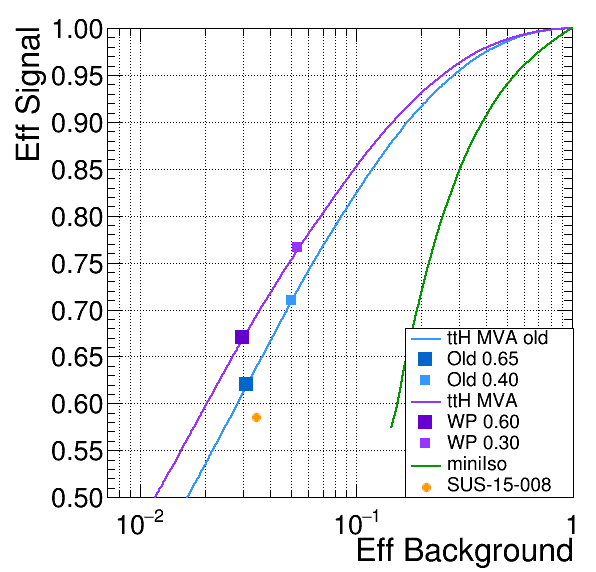
\includegraphics[width=0.40\linewidth]{plots_lepMVA/el_pt_10_25.png}
%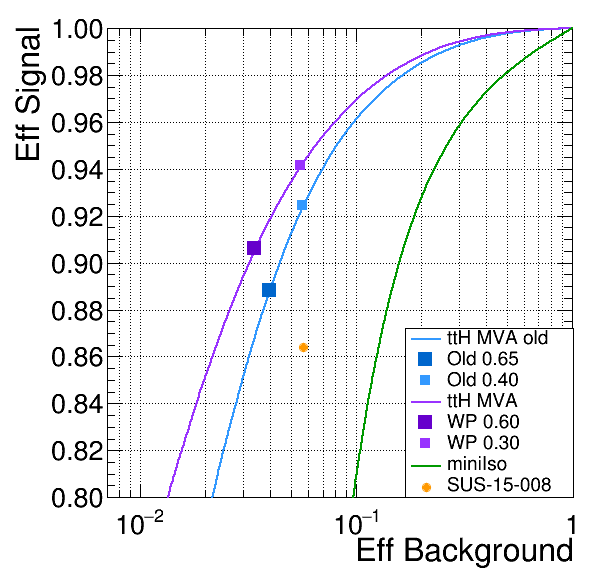
\includegraphics[width=0.40\linewidth]{plots_lepMVA/el_pt_25_inf.png} \\
%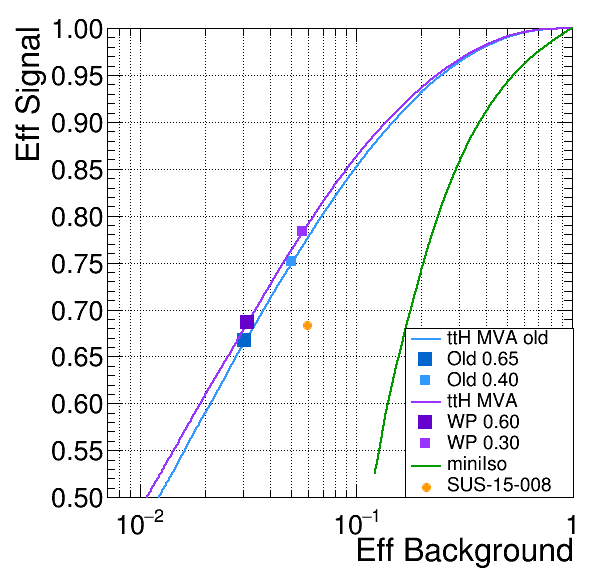
\includegraphics[width=0.40\linewidth]{plots_lepMVA/mu_pt_10_25.png}
%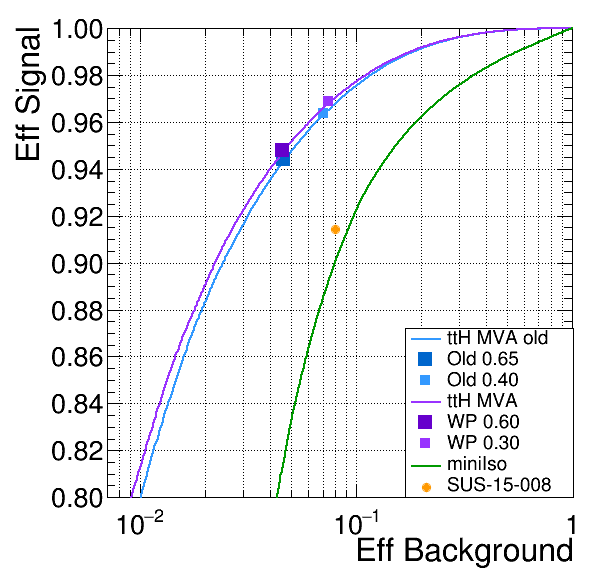
\includegraphics[width=0.40\linewidth]{plots_lepMVA/mu_pt_25_inf.png}
%\caption{The lepton MVA ROCs are shown from top left to bottom right
%for electrons with $10 < \pt < 25$, electrons with $\pt > 25$, muons
%with $10 < \pt < 25$, muons with $\pt > 25$. CMSSW 76X MC is used for this plot.}
%\label{fig:rocsMVA}
%\end{figure}


\subsubsection{Additional requirements}

In the dilepton final state additional requirements on the quality of
the charge assignment are applied to suppress opposite-sign events
in which the charge of one of the leptons is mismeasured. For the electrons we require
consistency between the independent measurements of the charge from
the ECAL supercluster and the tracker, while for the muons we require
the track transverse momentum to be well measured
($\Delta{p_{T}}/p_{T} <0.2$). We will refer to these cuts as \emph{tight-charge}\\
Moreover in order to suppress as much as possible background electrons
from photon conversions we reject electrons with missing hits in the
innermost layer or associated with a successfully reconstructed
conversion vertex~\cite{conversionRejection}.

\subsubsection{ \emph{Loose}, \emph{Fakeable Object}, \emph{Tight} definitions}
Three different selections are used both for the electron and the muon
objects identification: the \emph{Loose}, the \emph{Fakeable Object},
the \emph{Tight} selection. In the description of the analysis
strategy it will be explained for which purposes the different
criteria are used. \\
For reasons that will explained in the data-driven background prediction session,
for the Fakeable Object selections the lepton $\pt$ is
intended to $0.90*\pt(jet)$ with the jet being the one associated to the lepton as defined for the jet-related
variables computation.\\
In Table~\ref{tab:muonIDs} and Table~\ref{tab:eleIDs} all the criteria
on the variables previously described are listed.

\subsection{Validation of lepton identification variables}
We validate the modelling of the lepton identification variables in simulation by looking at three control regions: one enriched in prompt leptons from dileptonic \ttbar, one enriched in non-prompt leptons from semi-leptonic \ttbar, and one enriched in Z+jets events. The first control region is obtained selecting opposite-sign dilepton events with at least two jets and at least one medium b-tagged jet or two loose ones; events with more than two leptons are vetoed. The second control region is obtained selecting same-sign dilepton events with exactly three or four jets, and exactly one medium b-tagged jet, in order to suppress the contributions from $\ttbar\mathrm{V}$ and \ttH, and similarly events with more than two leptons are vetoed.
The third control region is obtained selecting same-flavor and opposite-sign pairs of leptons with higher than 25 and 15 GeV plus a third candidate with pT lower than 50 GeV, for which the transverse mass with the MET is lower than 55 GeV and the MET$<$60 GeV.
In all control regions, the trailing lepton is required only to pass the loose selection, not the lepMVA requirement, so that its properties can be studied in an unbiased way.
A data to simulation comparison is done for the lepton MVA discriminant and some of the more important inputs: the mini-isolation, $\mbox{SIP}_{3D}$, $\ptRatio$, $\ptRel$ and the b-tagging discriminator of the associated jet (Fig.~\ref{fig:lep-distributions-1} and ~\ref{fig:lep-distributions-2}). In all cases, the simulation is normalized to data, scaling all contributions by the same factor. The contribution from \ttbar is split according to the origin of the lepton in the simulation: prompt, non-prompt from B hadron decays ($\cPqb\to\ell_\mathrm{np}$), or non-prompt from other origins  ($\mathrm{j}\to\ell_\mathrm{np}$).
A good agreement between data and simulations is observed overall, while minor discrepancies may be related to the fact that no corrections are applied to the simulation.
% Some small discrepancy is visible mainly for extreme values of the b-tagging discriminator and small $\mbox{SIP}_{3D}$ for non-prompt leptons, which could be also be partially from different relative abunances of leptons from heavy flavour vs light flavour processes in data with respect to simulations, or a slightly different levels of prompt lepton contamination.

\begin{table}[h!]
\centering
\small
\topcaption{
\label{tab:muonIDs}
Requirements on each of the three muon selections. In the cases where
the cut values change between the selections, those values are listed in the table.
Otherwise, whether the cut is applied is indicated.
A few extra requirements are applied for fakeable objects that fail the lepton MVA requirement, to better control the extrapolation in fragmentation and flavour composition: $\ptRatio > 0.5$ (for all), jet $\textrm{CSV} < 0.3$, segmentCompatibility$>$0.3 for muons, electron ID $\textrm{MVA} > 0.0 (0.7)$ for electrons in the barrel (endcaps).}
\begin{tabular}{c|c|c|c}
\hline
\bf{Cut} & \bf{Loose} & \bf{Fakeable Object} & \bf{Tight} \\
\hline
$|\eta| < 2.4$ & \checkmark & \checkmark & \checkmark \\
$\pt$ & $>5$ & $>15$ & $>15$\\
$|d_{xy}| < 0.05$ (cm) & \checkmark & \checkmark & \checkmark \\
$|d_z| < 0.1$ (cm) & \checkmark & \checkmark & \checkmark \\
$\text{SIP}_{3D} < 8$ & \checkmark & \checkmark & \checkmark \\
\miniIso $< 0.4$ & \checkmark & \checkmark & \checkmark \\
is Loose Muon & \checkmark & \checkmark & \checkmark \\
%\ptRatio & -- & $>0.3\dagger$ / -- &  -- \\
jet CSV  & -- & $< 0.8484$ & $ < 0.8484$ \\
%mva electron ID  & -- & $\ddagger$ & -- \\
is Medium Muon & -- & -- & \checkmark \\
tight-charge & -- & -- & \checkmark \\
lepMVA $> 0.90$ & -- & -- & \checkmark \\
\hline
\end{tabular}
\end{table}


\begin{table}
\centering
\small
\topcaption{
\label{tab:eleIDs}
Requirements on each of the three electron selections. In the cases where the cut values change between the selections, those values are listed in the table. Otherwise, whether the cut is applied is indicated. In some cases, the cut values change for different $\eta$ ranges. These ranges are $0 < |\eta| < 0.8$, $0.8 < |\eta| < 1.479$, and $1.479 < |\eta| < 2.5$ and the respective cut values are given in the form (value$_1$, value$_2$, value$_3$). Cuts marked with $\dagger$ are applied only to objects failing the tight selection.
}
\resizebox{1.0\linewidth}{!}{
\begin{tabular}{c|c|c|c}
\hline
\bf{Cut} & \bf{Loose} & \bf{Fakeable Object} & \bf{Tight} \\
\hline
$|\eta| < 2.5$ & \checkmark & \checkmark & \checkmark \\
$\pt$ & $>7$ & $>15$ & $>15$ 2lss(3l) \\
$|d_{xy}| < 0.05$ (cm) & \checkmark & \checkmark & \checkmark \\
$|d_z| < 0.1$ (cm) & \checkmark & \checkmark & \checkmark \\
$\text{SIP}_{3D} < 8$ & \checkmark & \checkmark & \checkmark \\
\miniIso $< 0.4$ & \checkmark & \checkmark & \checkmark \\
MVA ID $> (0.0, 0.0, 0.7)$ & \checkmark & \checkmark & \checkmark \\
$\sigma_{i\eta i\eta} <(0.011,0.011,0.030)$ & -- & \checkmark & \checkmark \\ %& for corr. $\pt>30$ & for corr. $\pt>30$ \\
H/E $< (0.10,0.10,0.07)$ & -- & \checkmark & \checkmark \\ %& for corr. $\pt>30$ & for corr. $\pt>30$ \\
$\Delta\eta_{\textrm in} < (0.01, 0.01, 0.008)$ & -- & \checkmark & \checkmark \\ %& for corr. $\pt>30$ & for corr. $\pt>30$ \\
$\Delta\phi_{\textrm in} < (0.04, 0.04, 0.07)$ & -- & \checkmark & \checkmark \\ %& for corr. $\pt>30$ & for corr. $\pt>30$ \\
$-0.05 < 1/E-1/p < (0.010,0.010,0.005)$ & -- & \checkmark & \checkmark \\ %& for corr. $\pt>30$ & for corr. $\pt>30$ \\
\ptRatio & -- & $>0.5\dagger$ / -- & -- \\
jet CSV  & -- & $< 0.3 \dagger$ / $< 0.8484$ & $ < 0.8484$ \\
tight-charge & -- & -- & \checkmark \\
conversion rejection & -- & -- & \checkmark \\
Number of missing hits & $<2$ & $== 0$ & $== 0$ \\
lepMVA $> 0.90$ & -- & -- & \checkmark \\
\hline
\end{tabular}}
\end{table}

\begin{figure}
        \centering
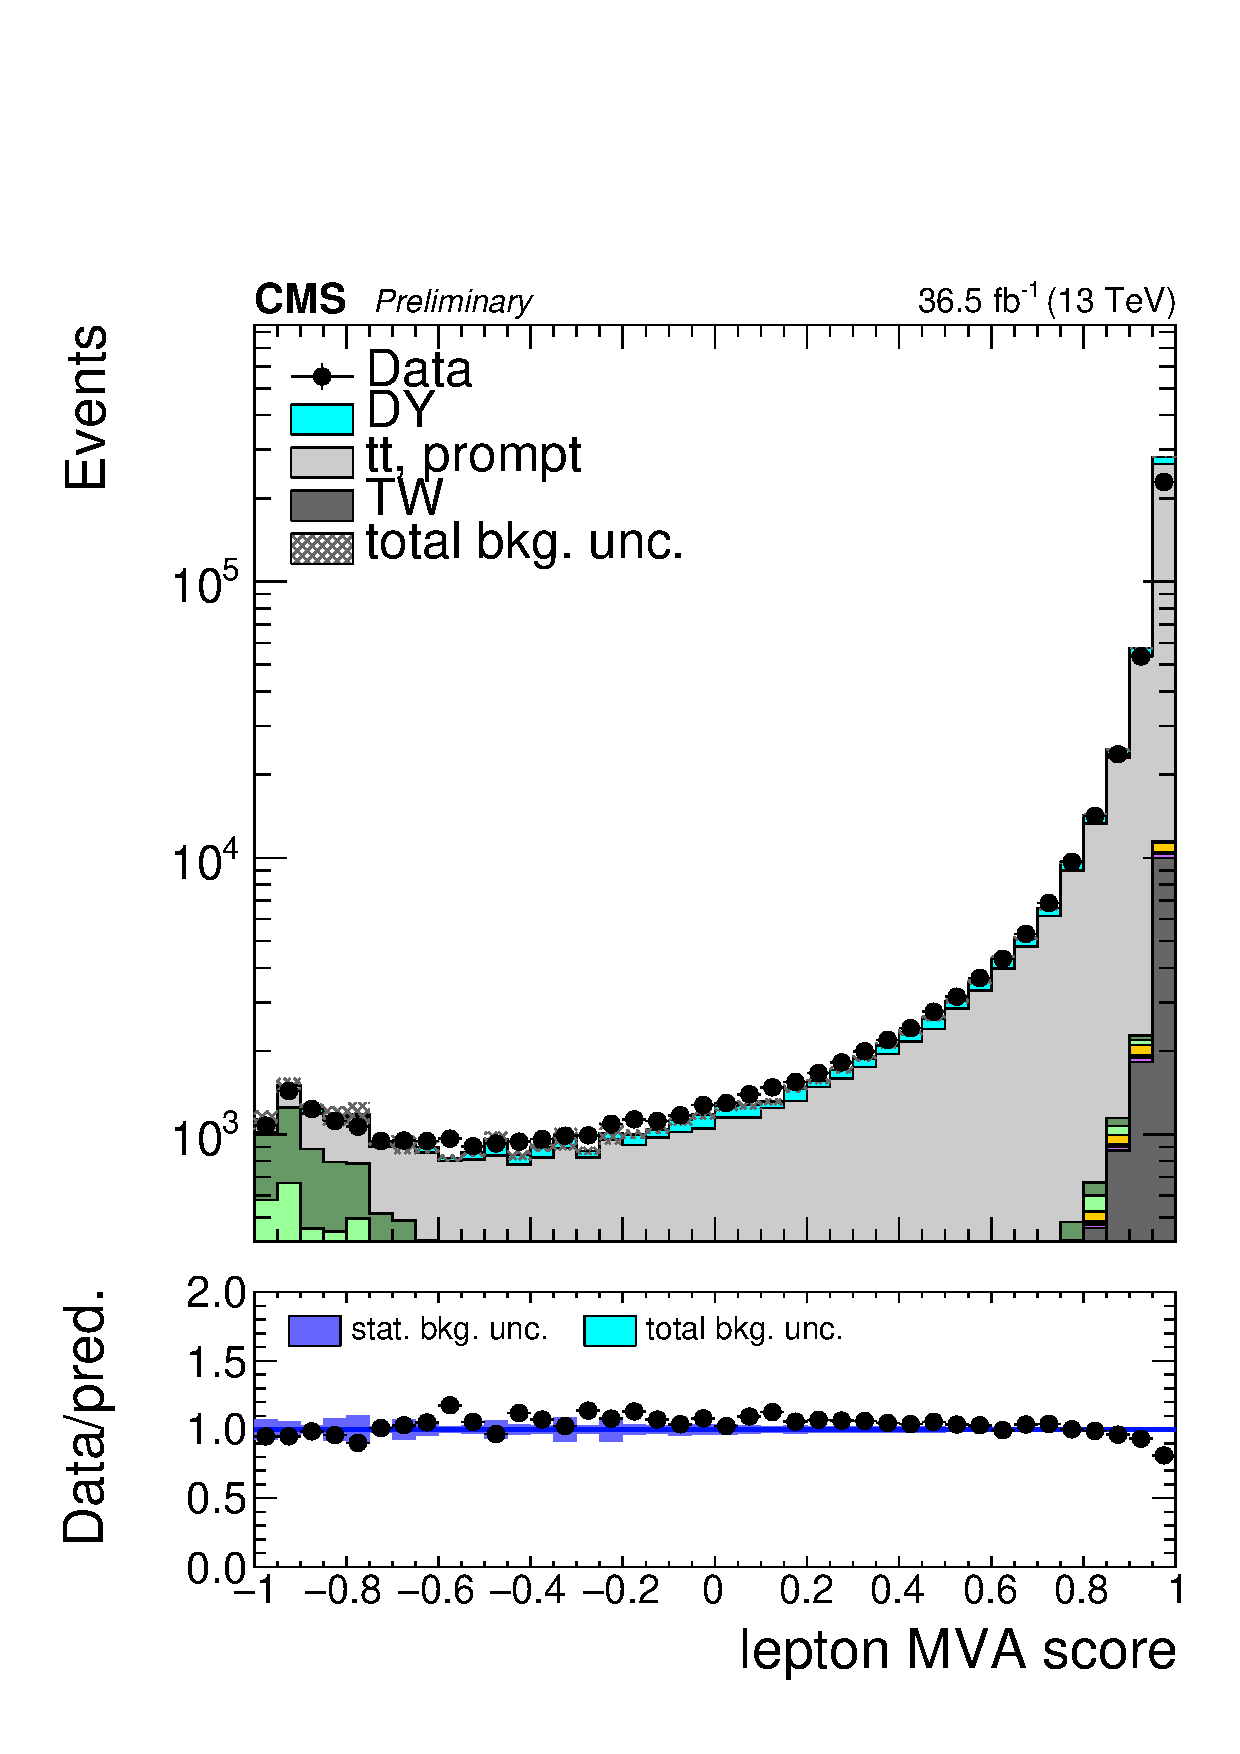
\includegraphics[width=0.32\textwidth]{plots_controlregions/leptons/lep_mvaTTH_log_prompt.pdf}
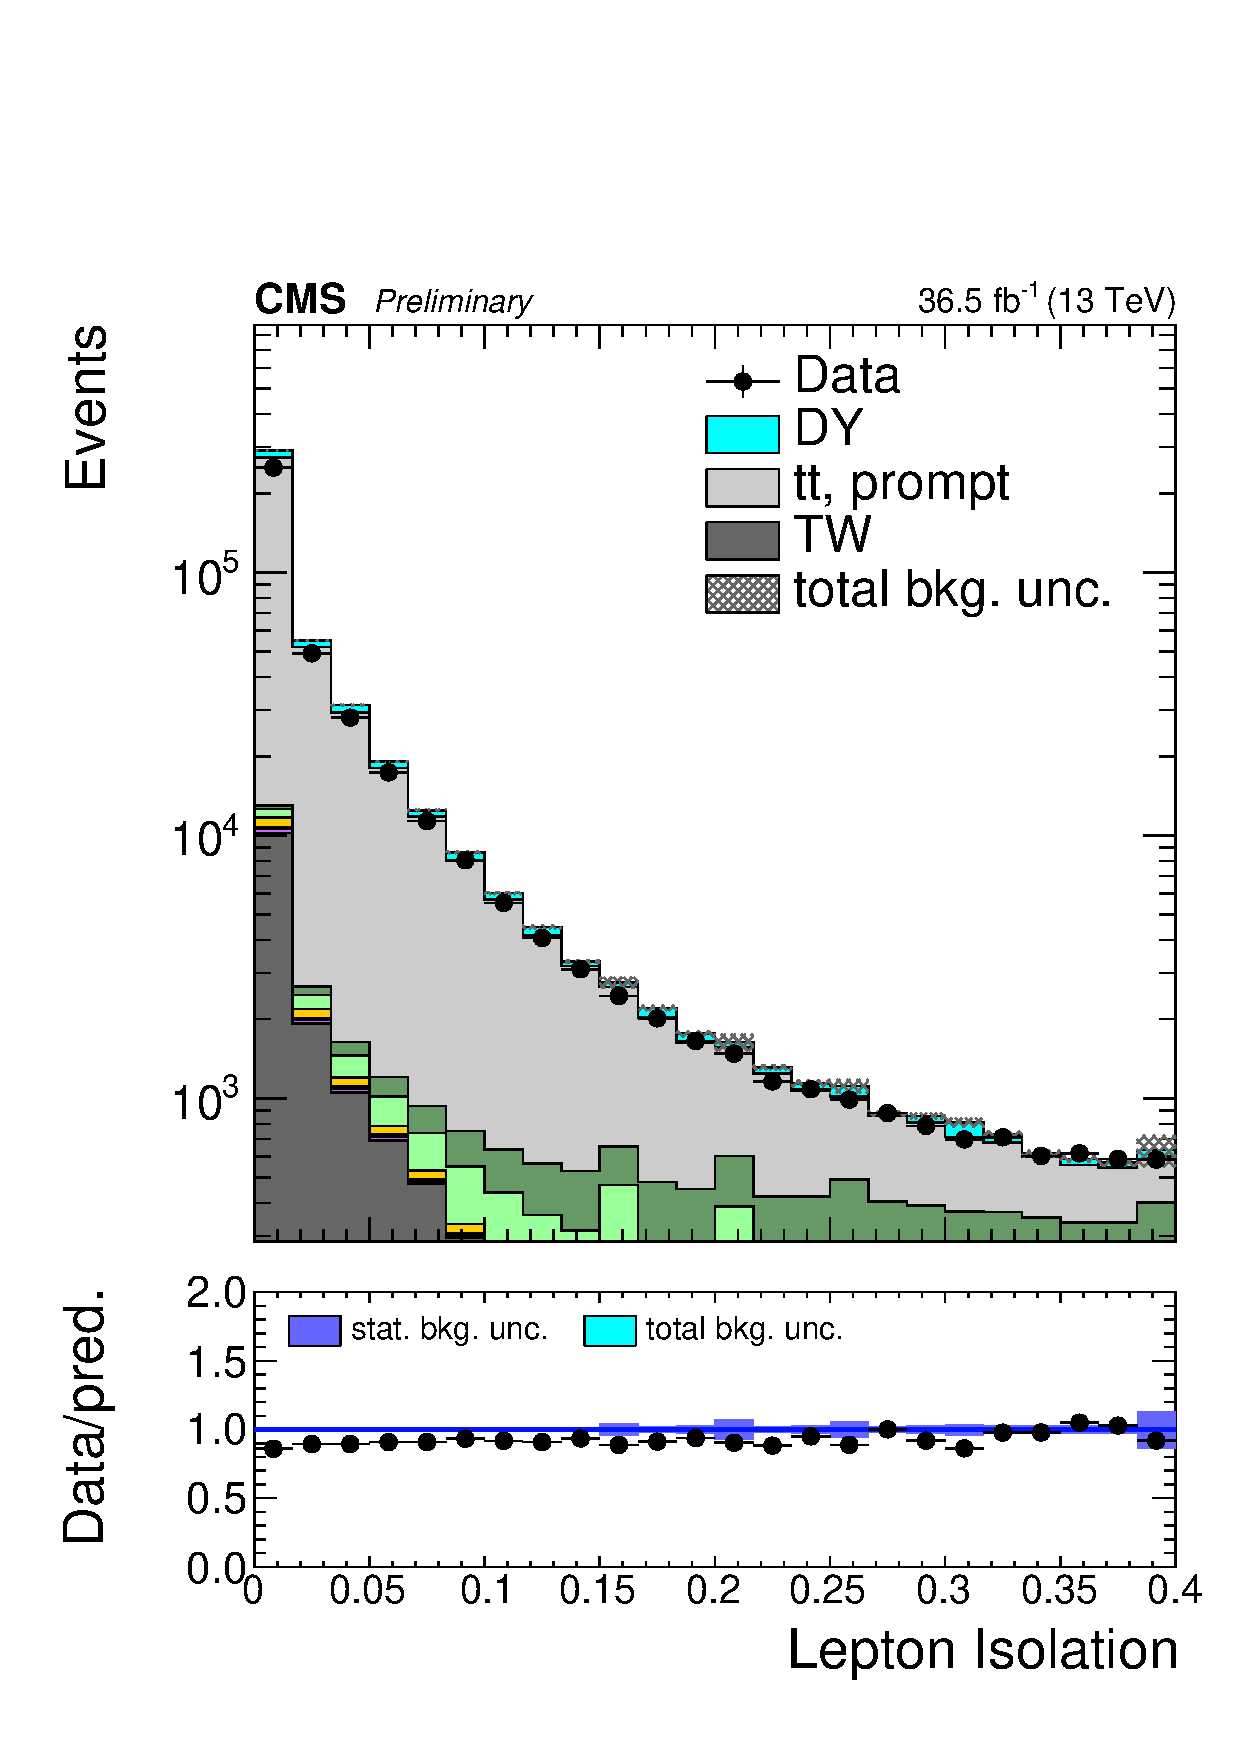
\includegraphics[width=0.32\textwidth]{plots_controlregions/leptons/lep_miniRelIso_log_prompt.pdf}
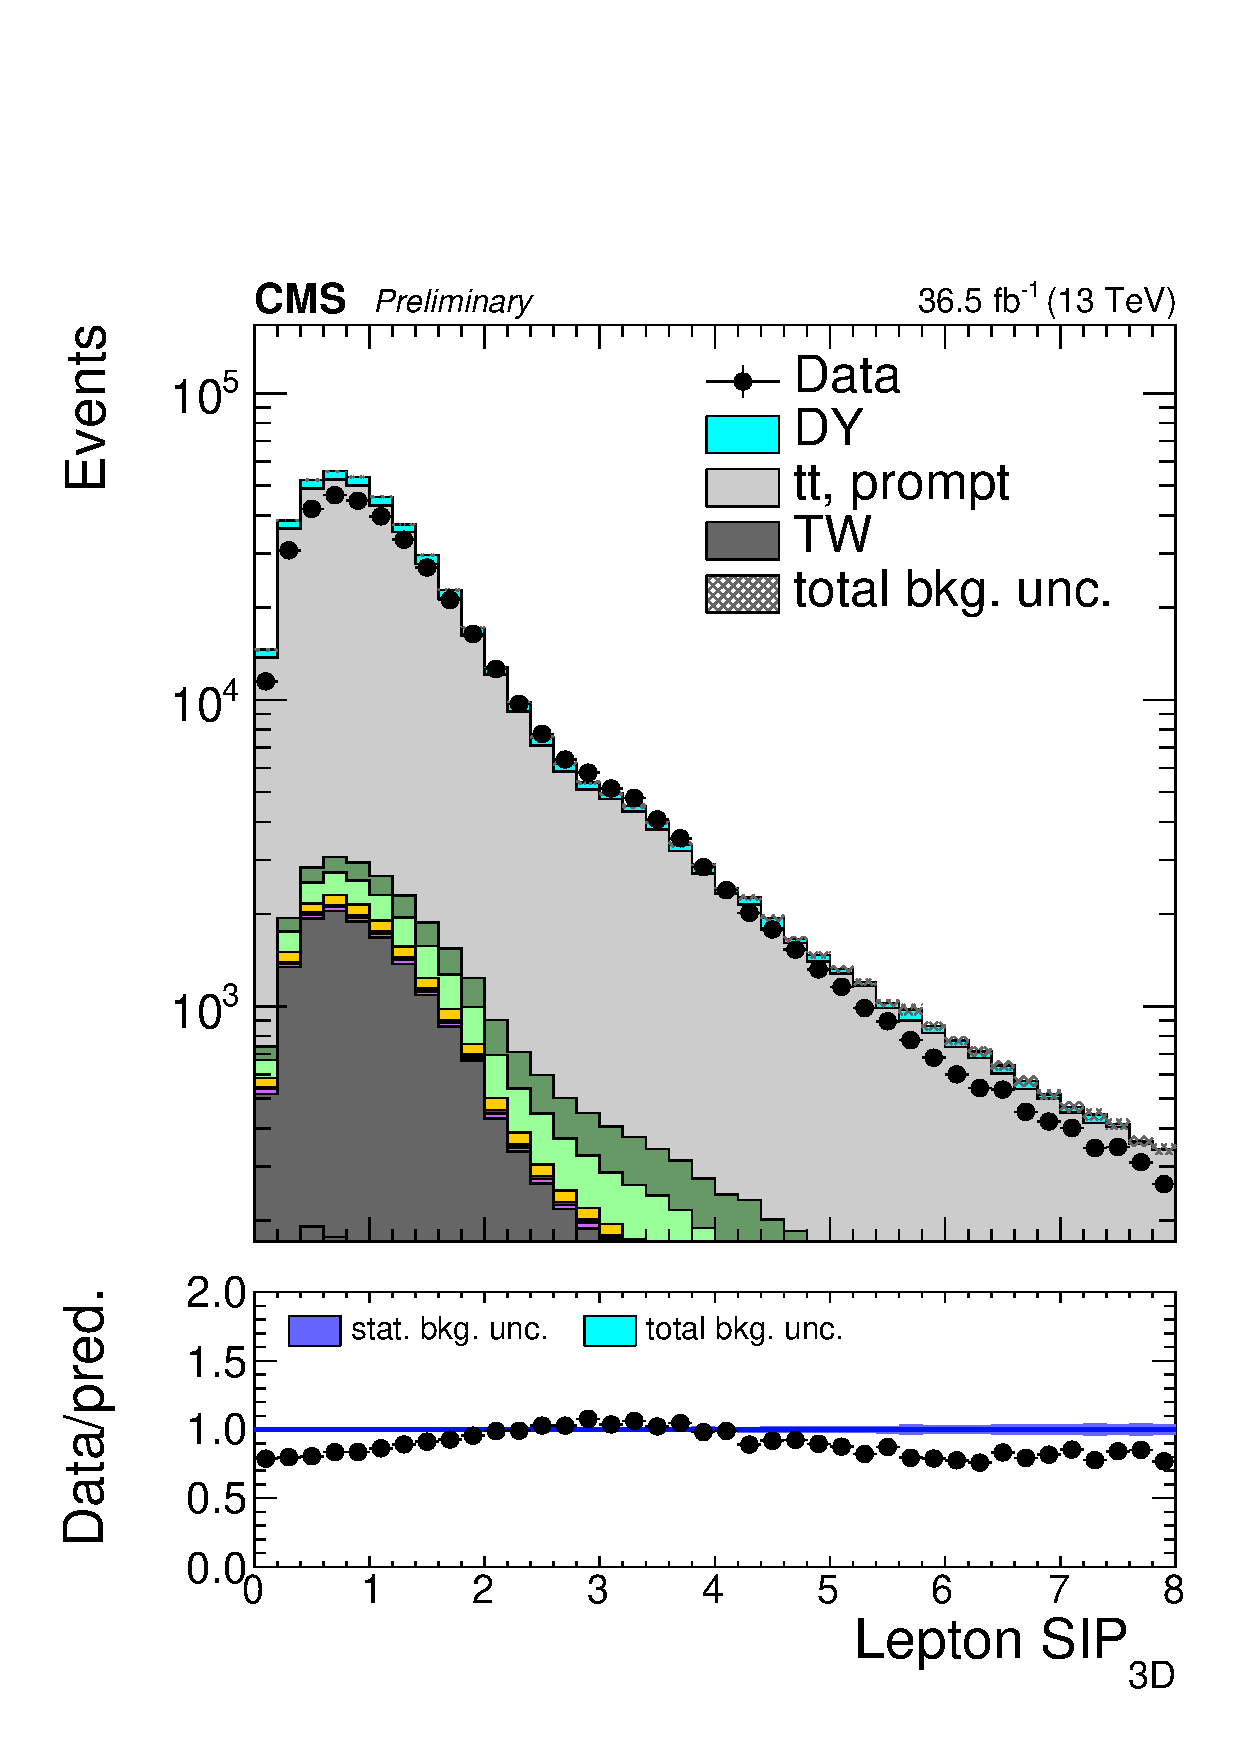
\includegraphics[width=0.32\textwidth]{plots_controlregions/leptons/lep_sip3d_log_prompt.pdf}\\
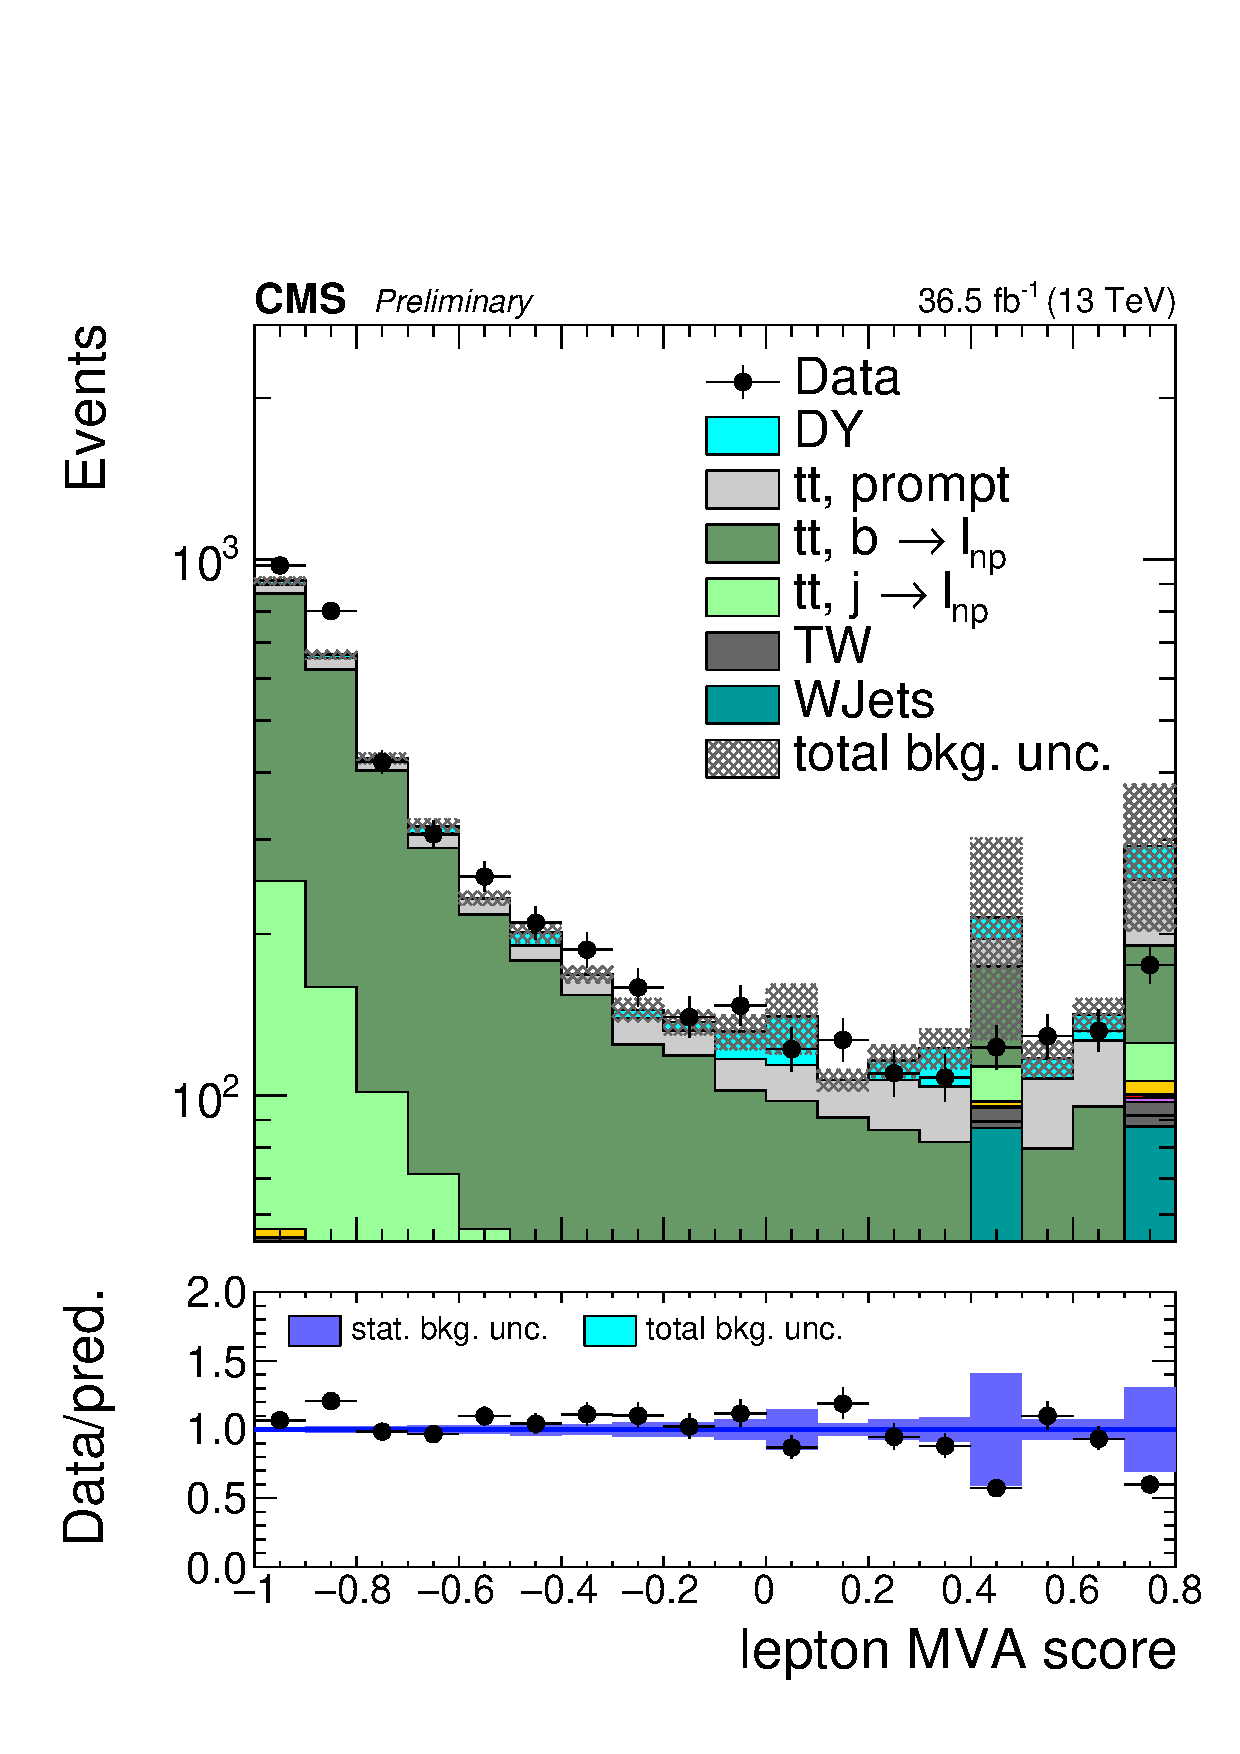
\includegraphics[width=0.32\textwidth]{plots_controlregions/leptons/lep_mvaTTH_log.pdf}
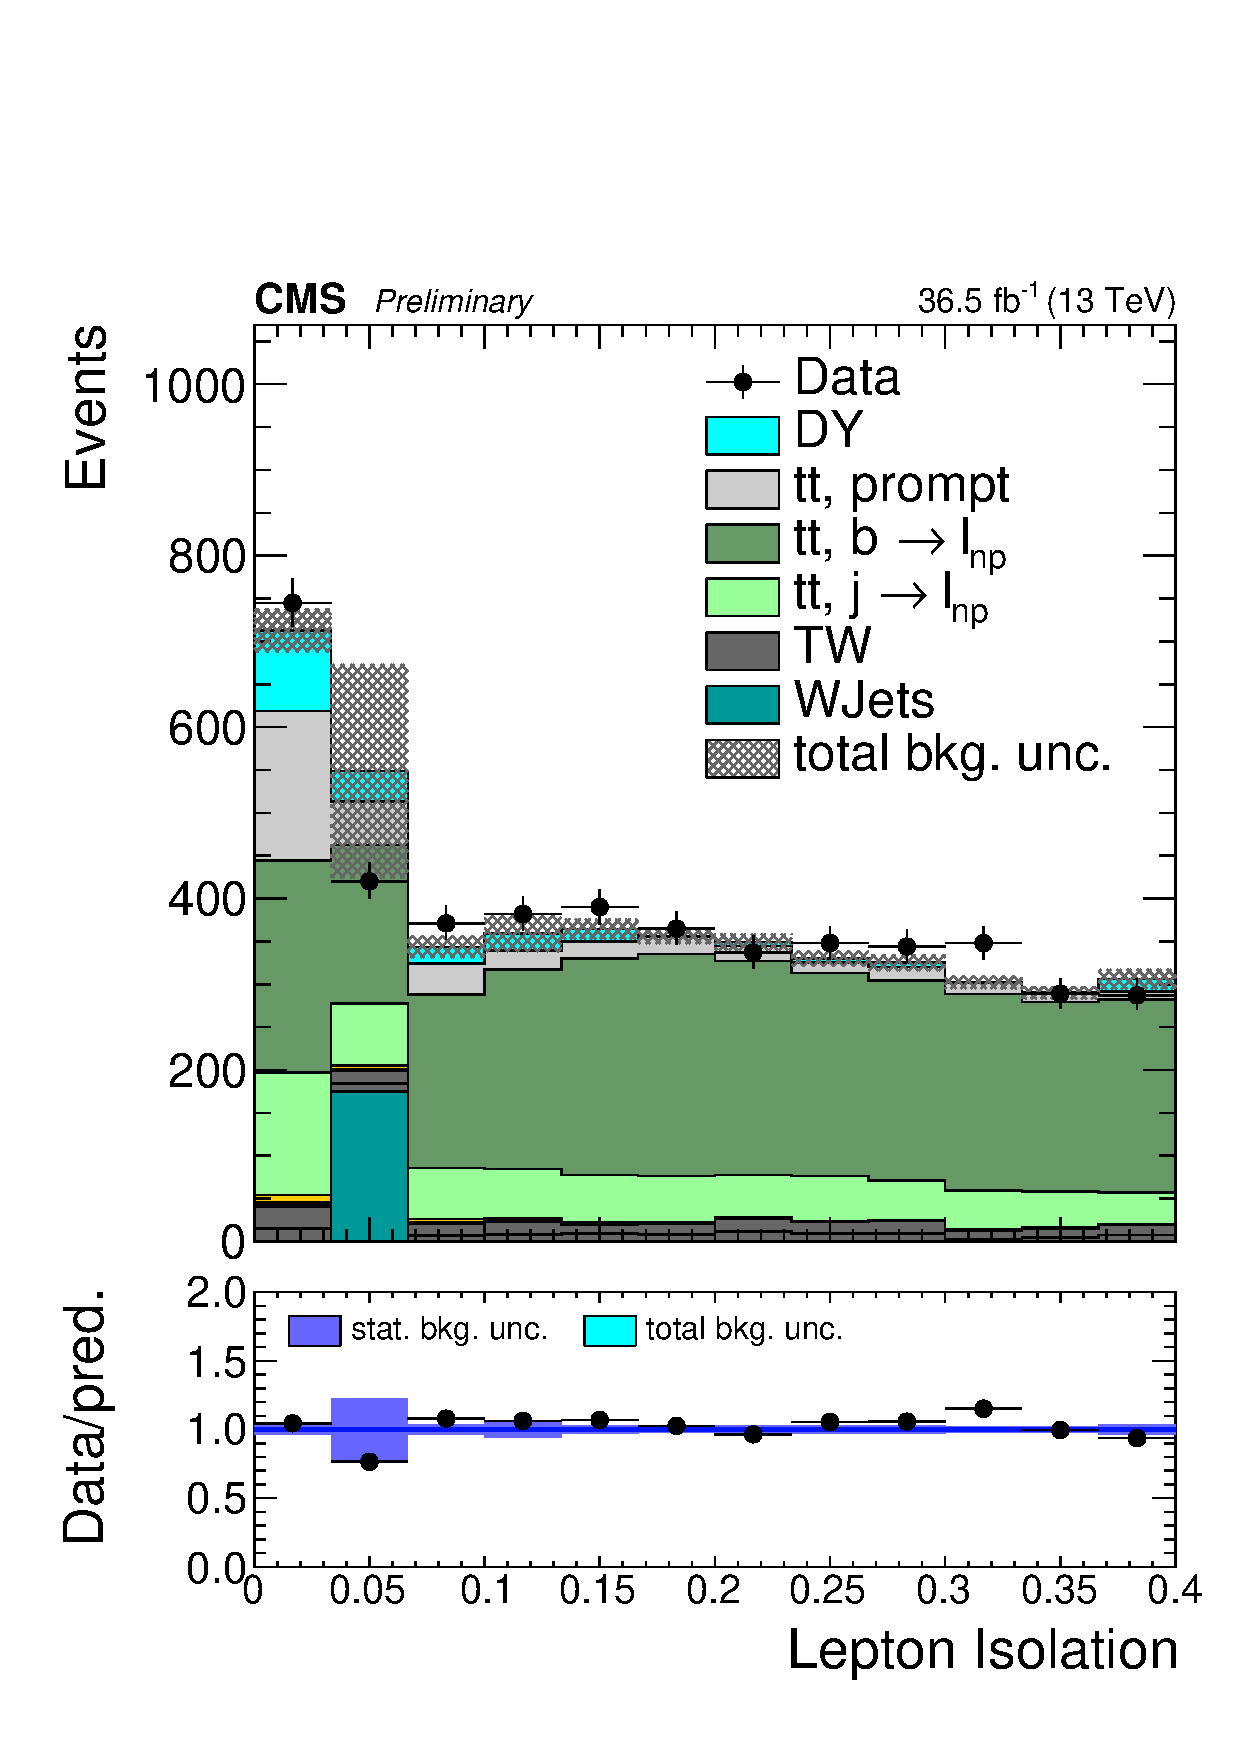
\includegraphics[width=0.32\textwidth]{plots_controlregions/leptons/lep_miniRelIso.pdf}
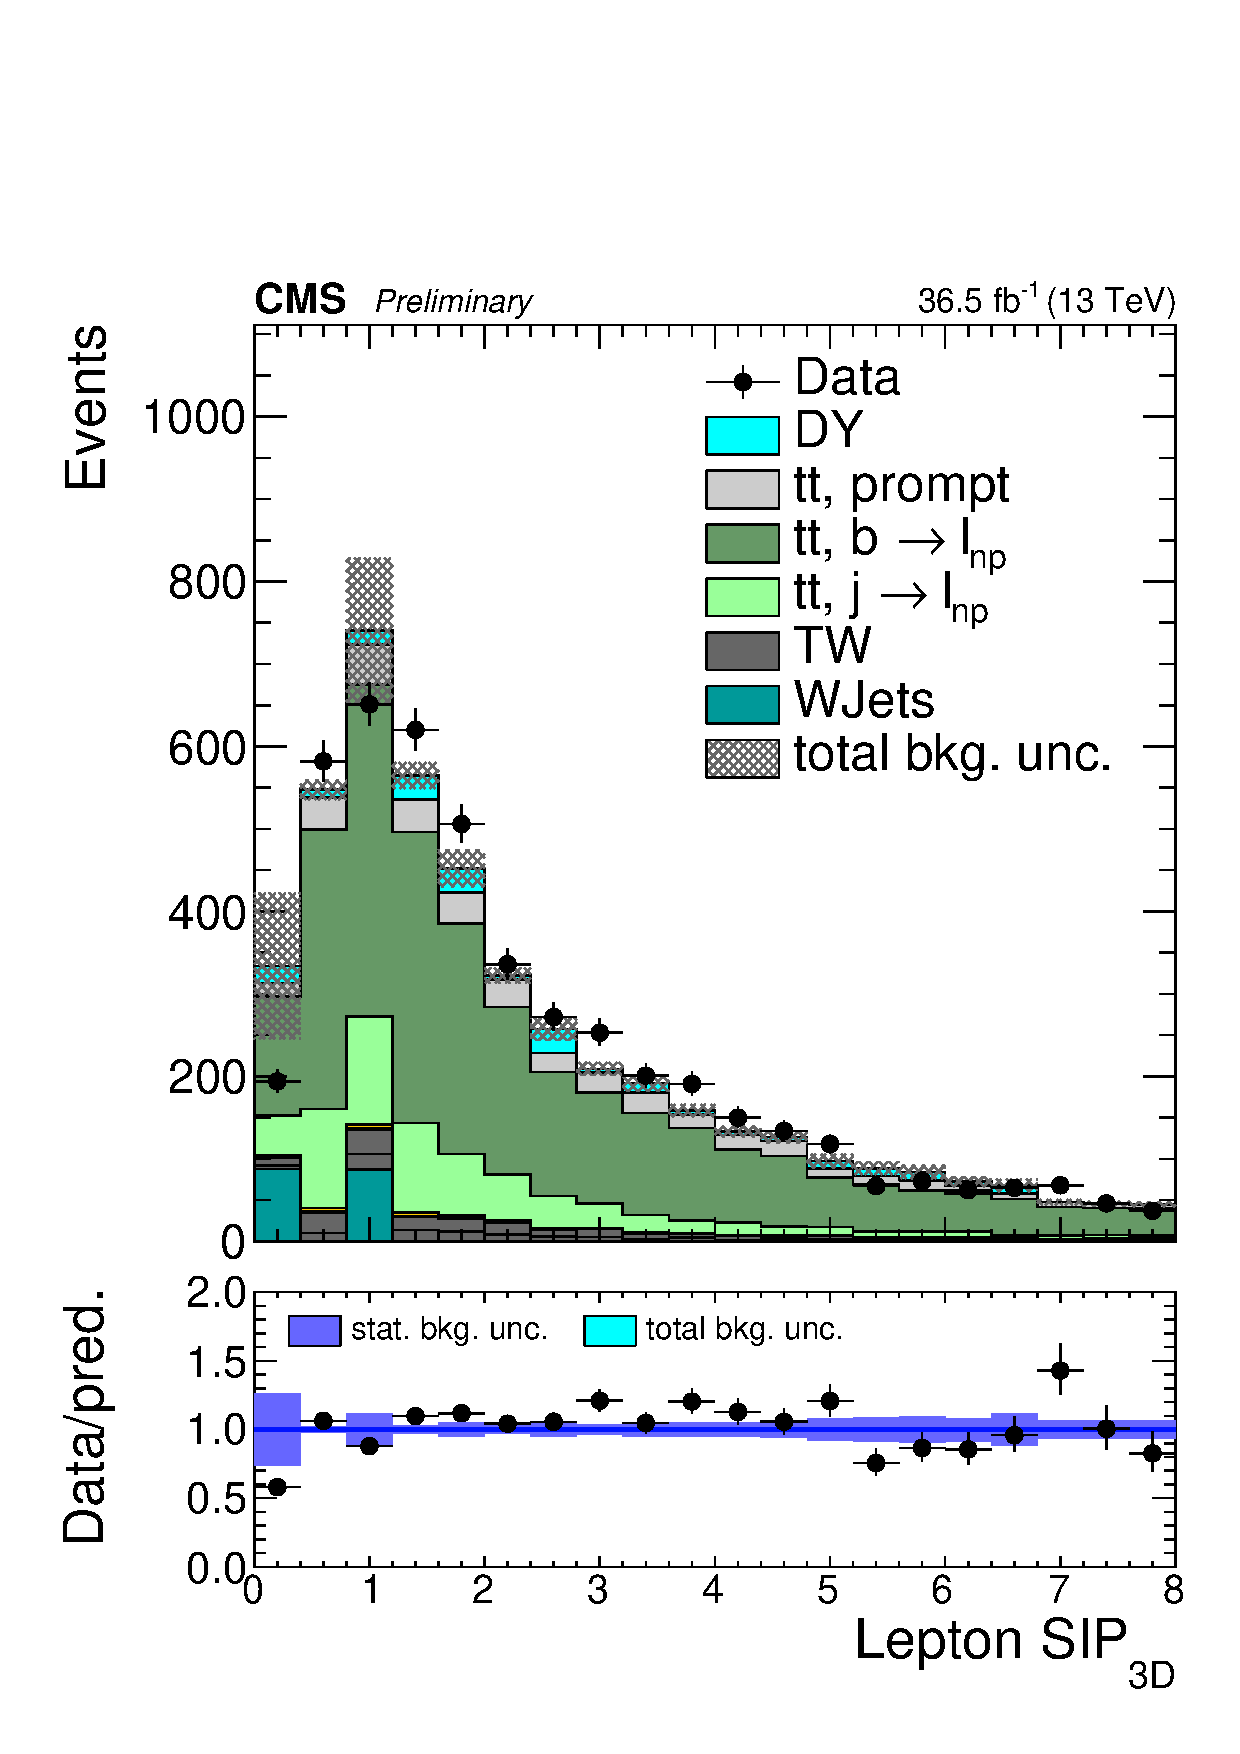
\includegraphics[width=0.32\textwidth]{plots_controlregions/leptons/lep_sip3d.pdf}\\
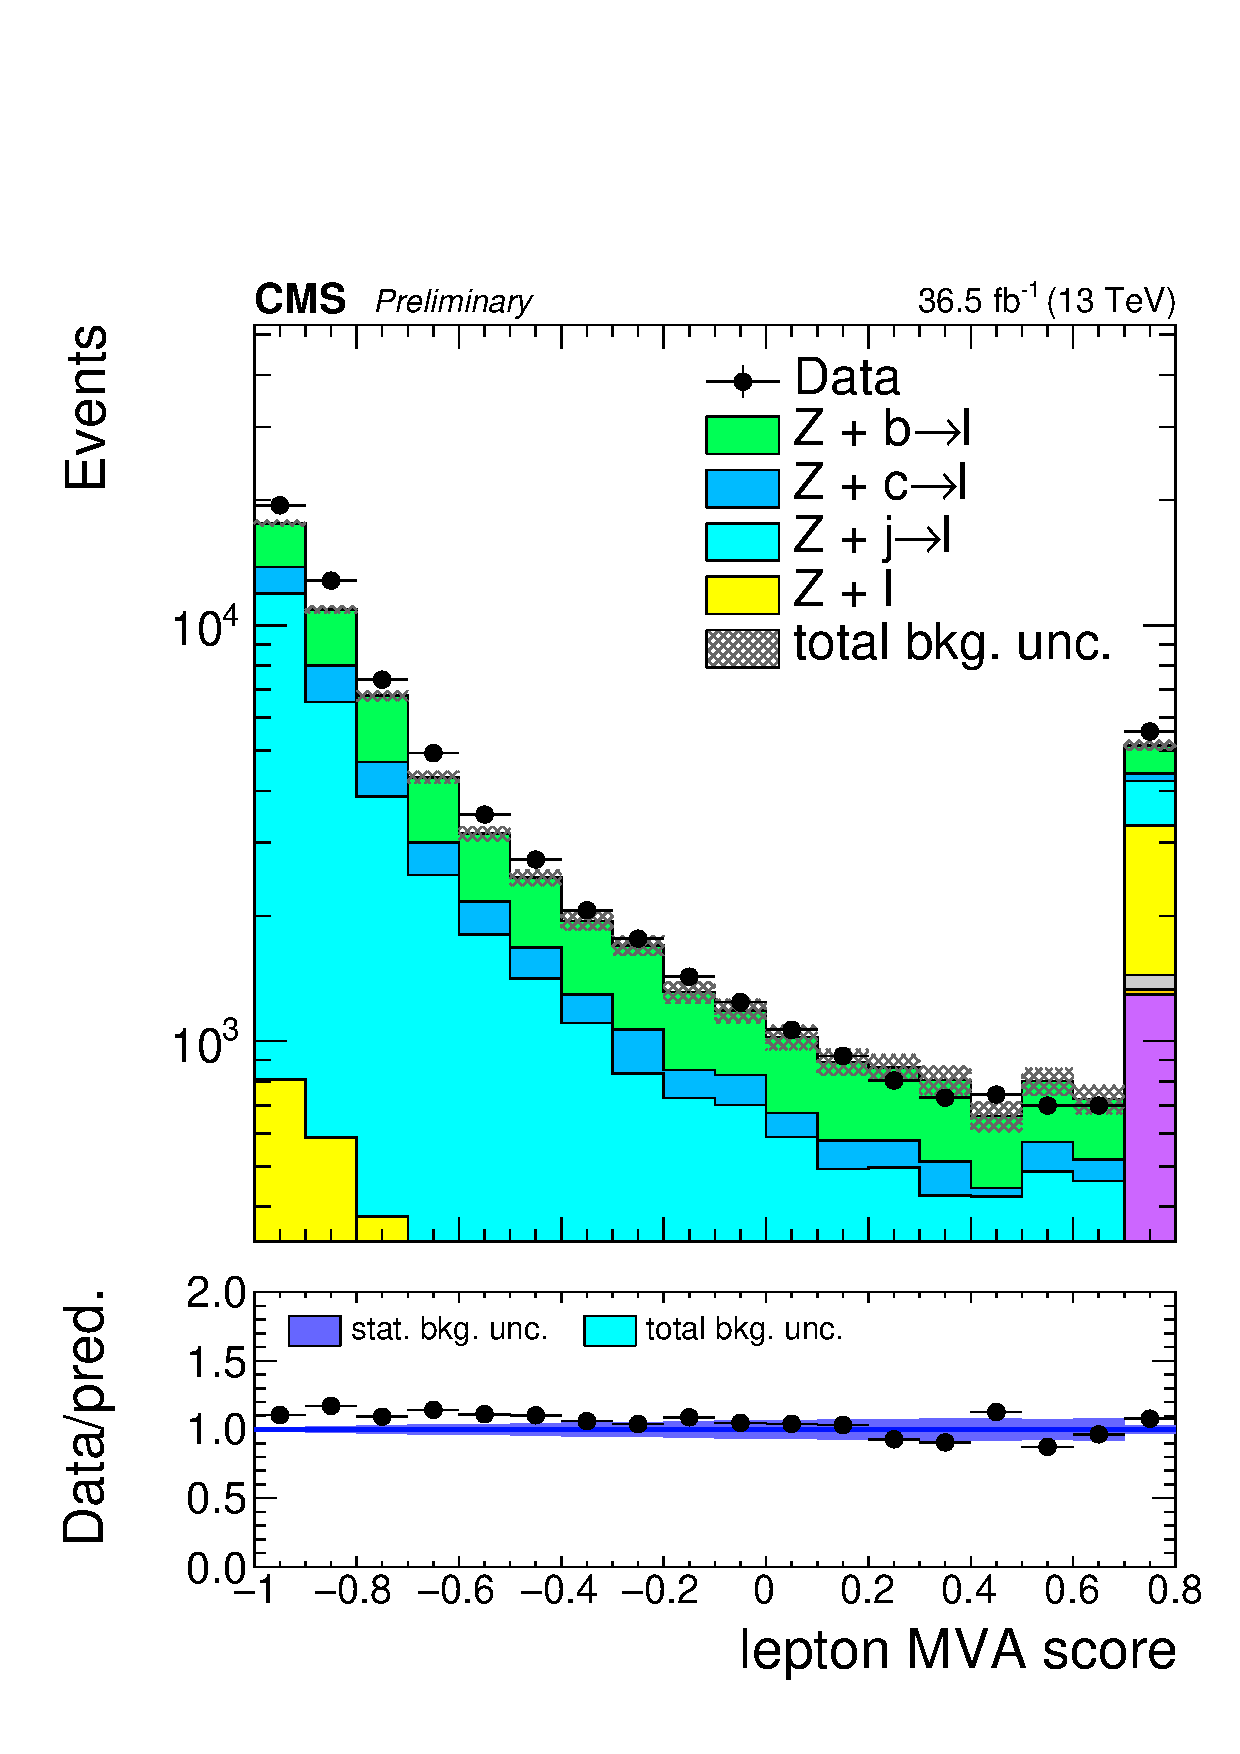
\includegraphics[width=0.32\textwidth]{plots_controlregions/leptons/lep_mvaTTH_log_Zl.pdf}
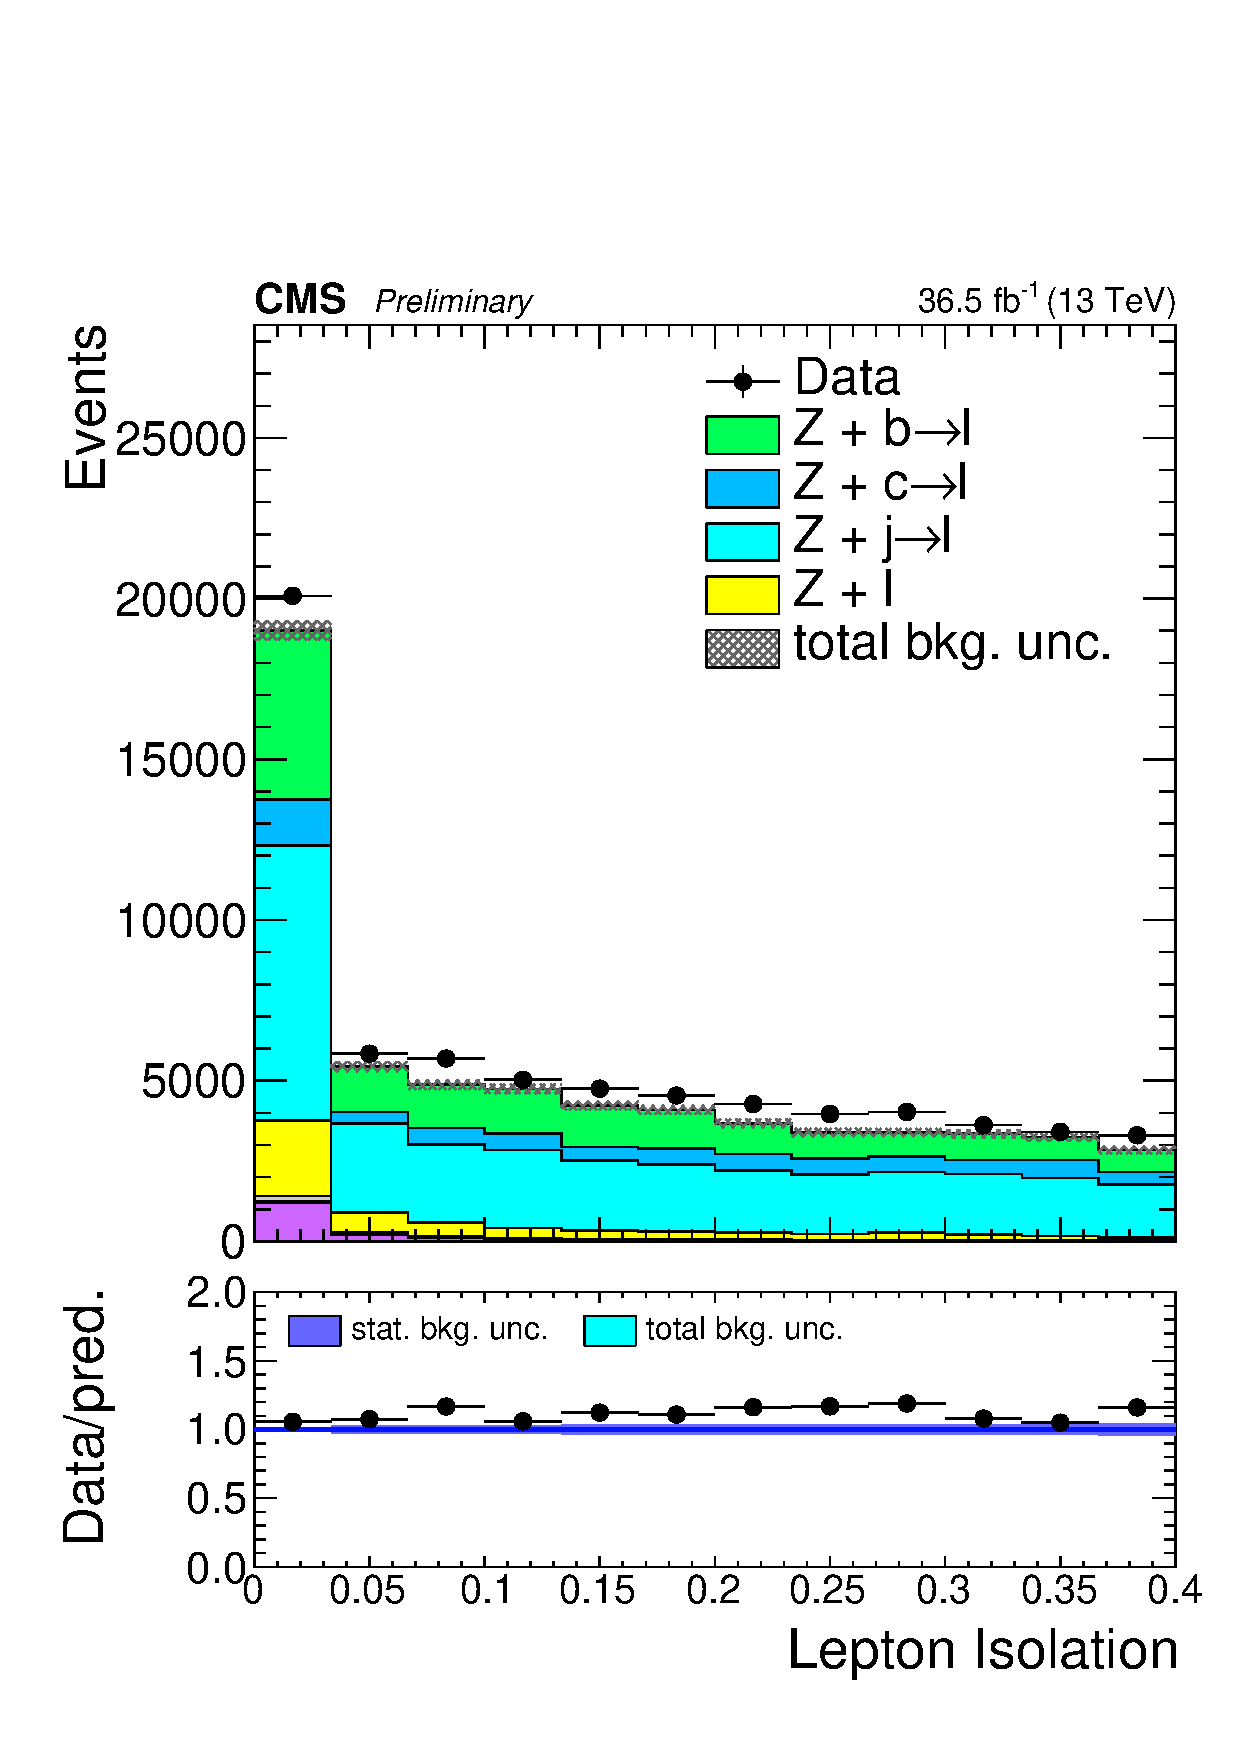
\includegraphics[width=0.32\textwidth]{plots_controlregions/leptons/lep_miniRelIso_Zl.pdf}
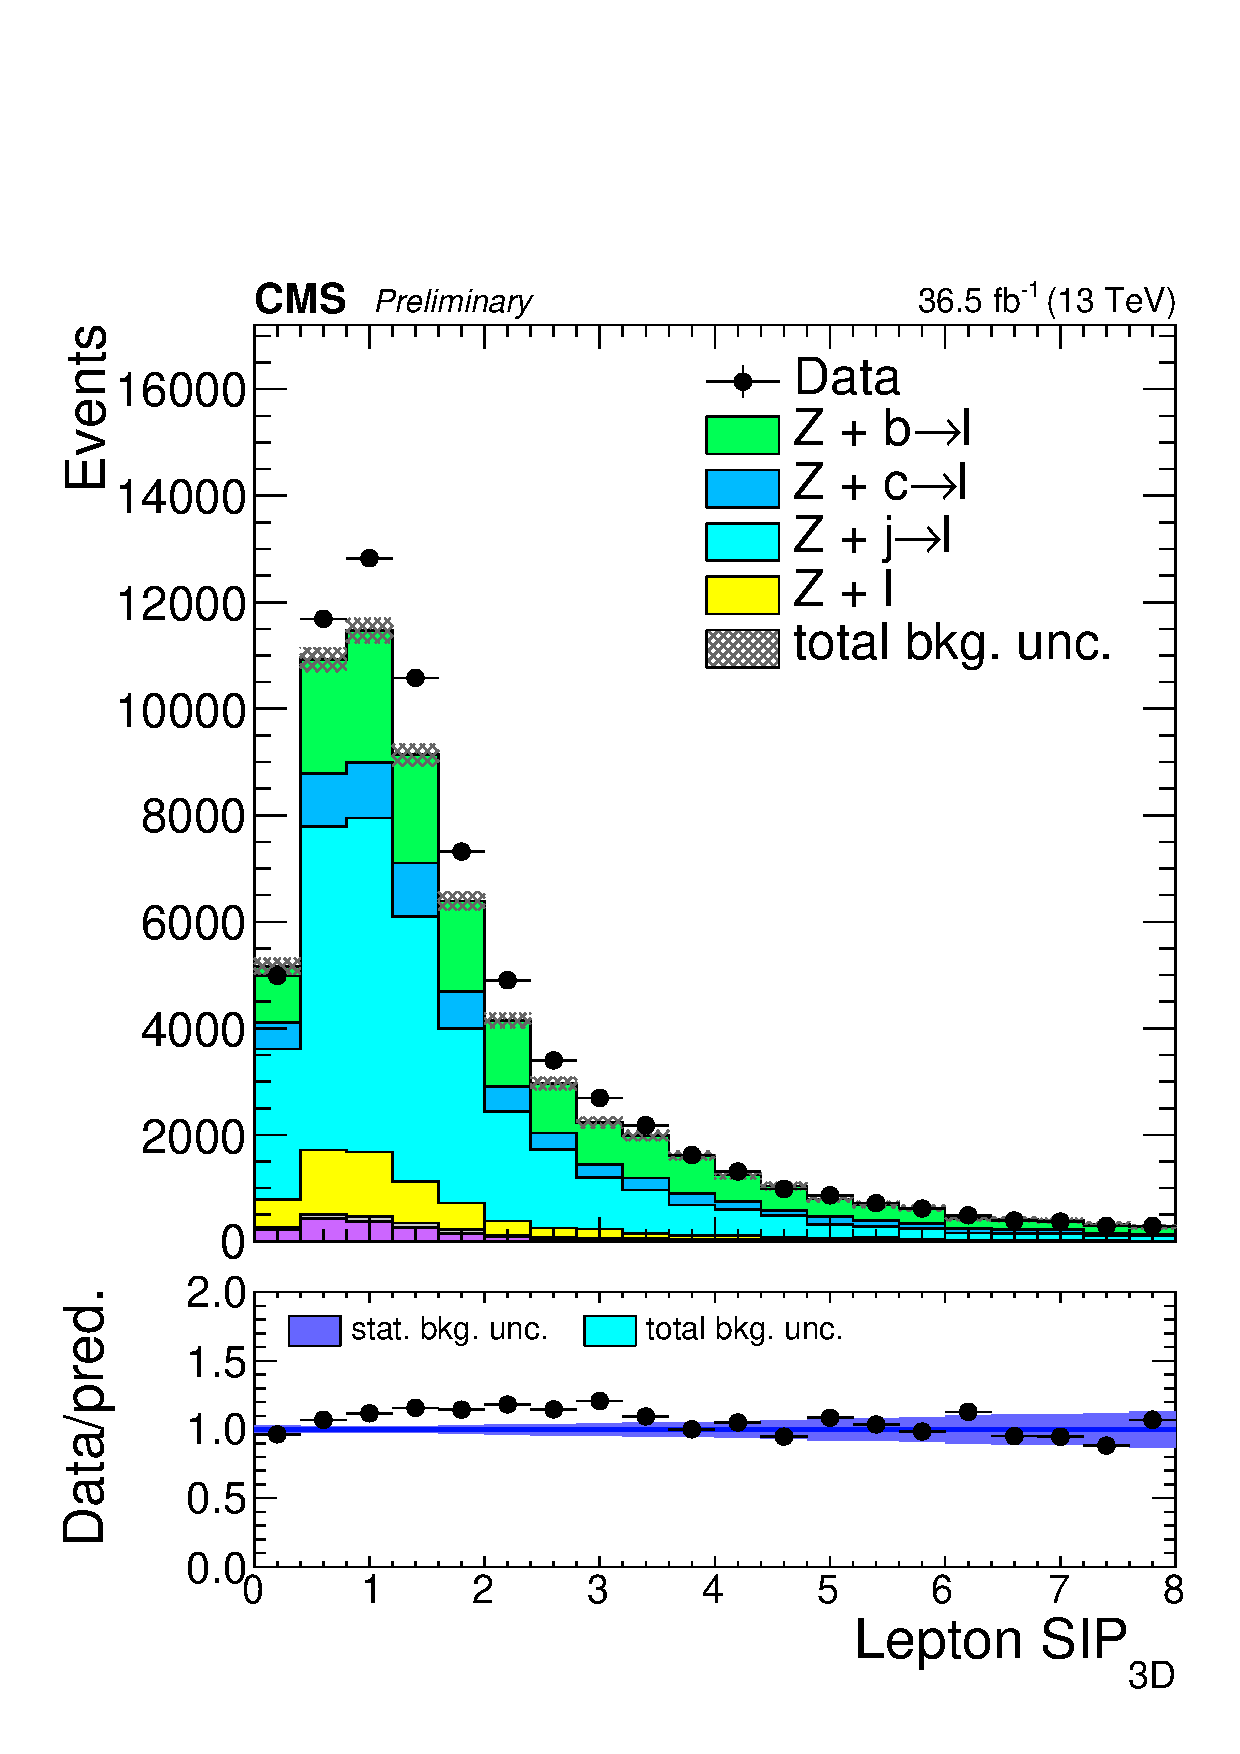
\includegraphics[width=0.32\textwidth]{plots_controlregions/leptons/lep_sip3d_Zl.pdf}
        \caption{Comparison of the distributions for the lepton MVA (left), mini-isolation (center), and $\mbox{SIP}_{3D}$ (right) between data and simulations in control regions enriched in prompt leptons (top), non-prompt leptons (center), and Z+jets events (bottom), as described in the text. The uncertainty shown on the simulation is only statistical.}
        \label{fig:lep-distributions-1}
\end{figure}

\begin{figure}
        \centering
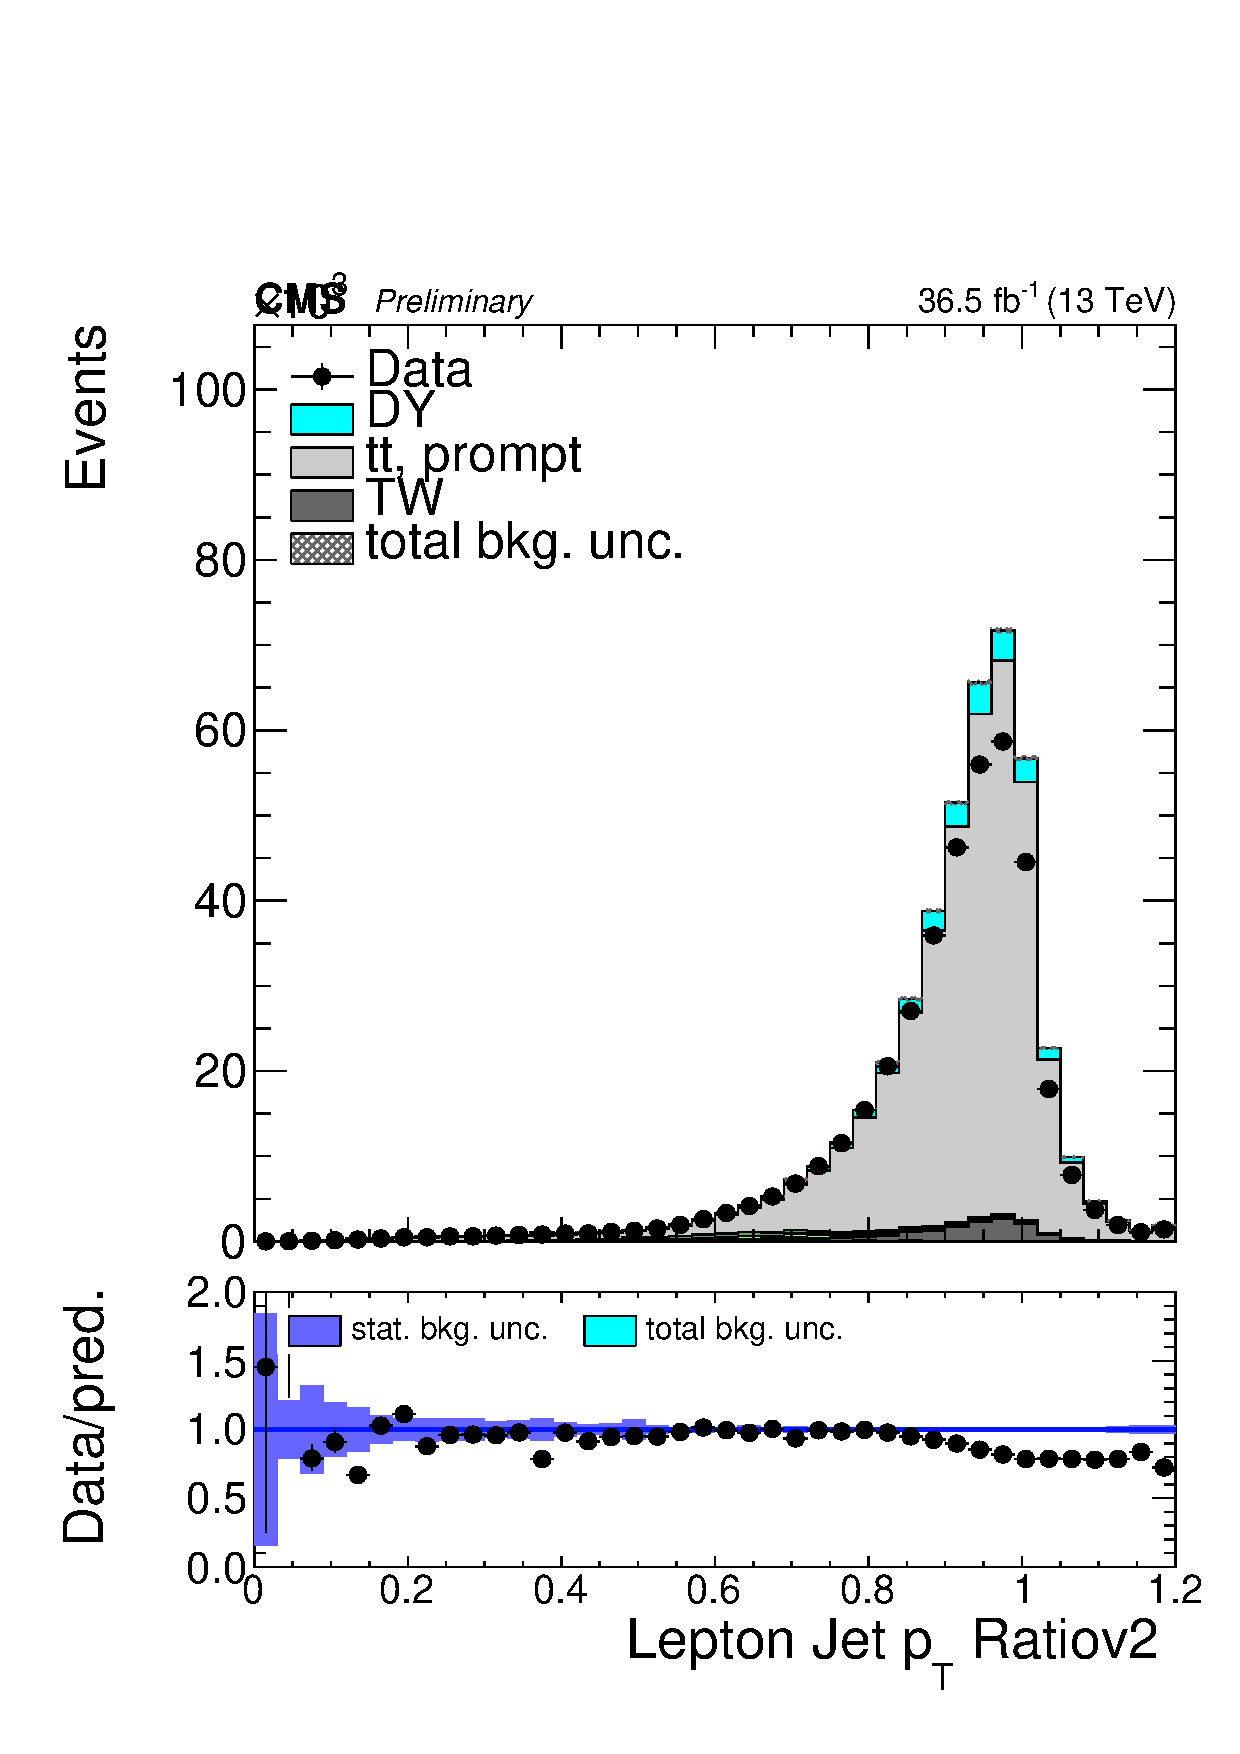
\includegraphics[width=0.32\textwidth]{plots_controlregions/leptons/lep_jetPtRatiov2_prompt.pdf}
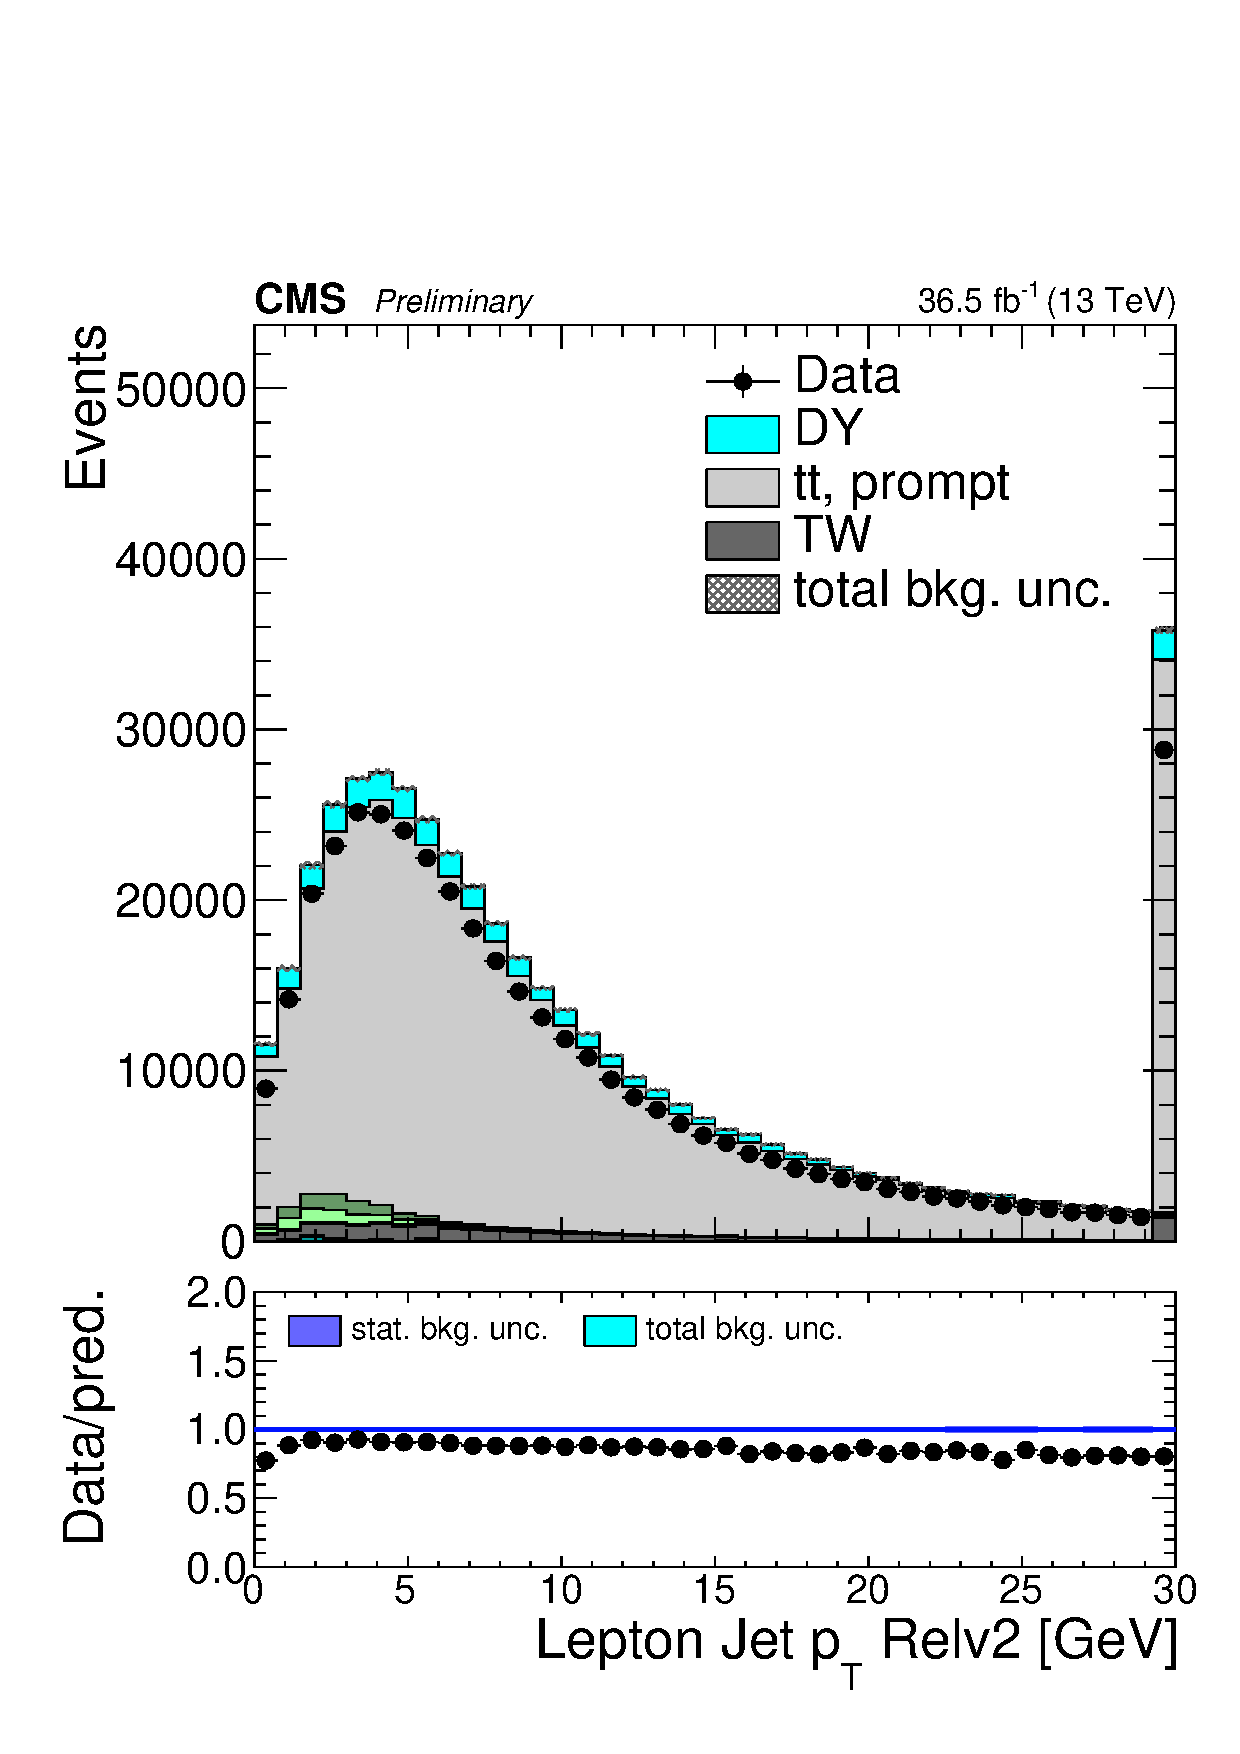
\includegraphics[width=0.32\textwidth]{plots_controlregions/leptons/lep_jetPtRelv2_prompt.pdf}
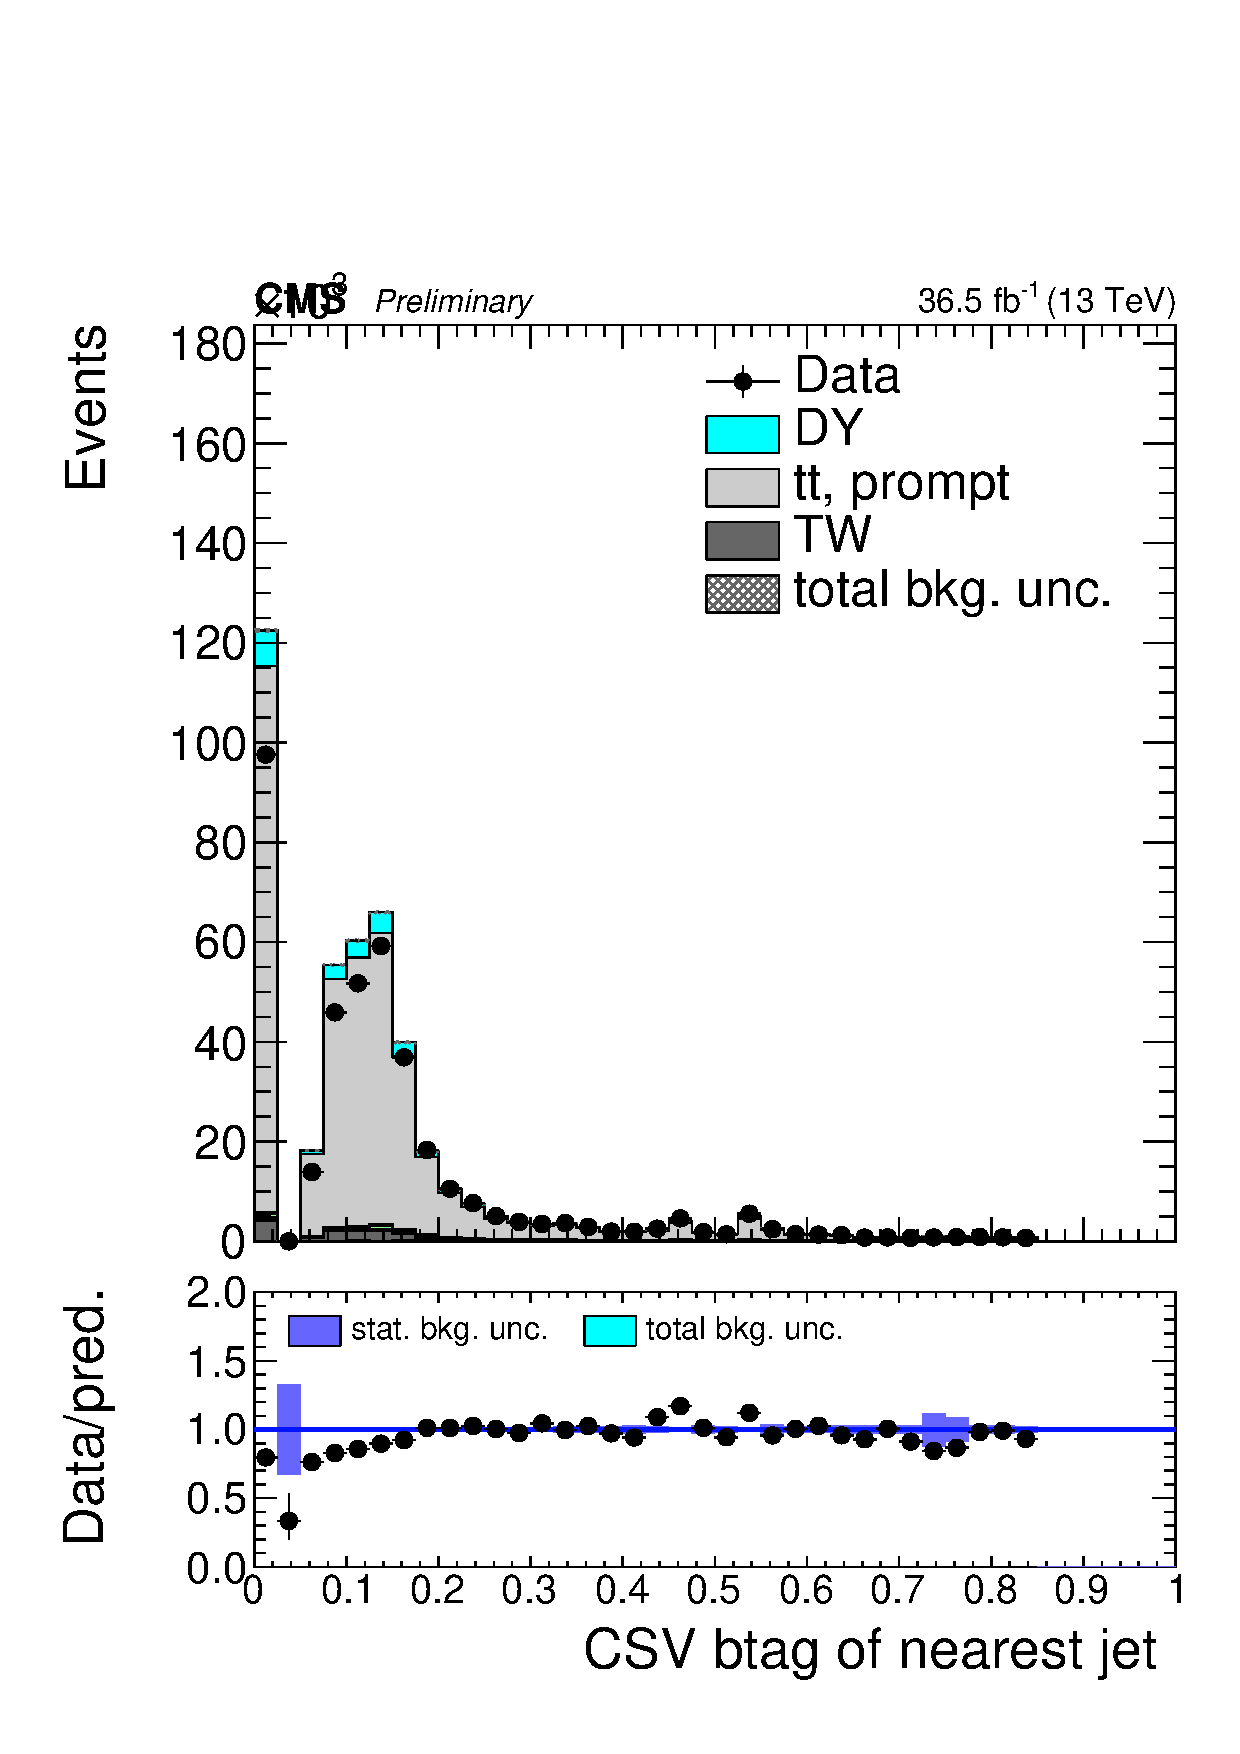
\includegraphics[width=0.32\textwidth]{plots_controlregions/leptons/lep_jetBTagCSV_prompt.pdf}\\
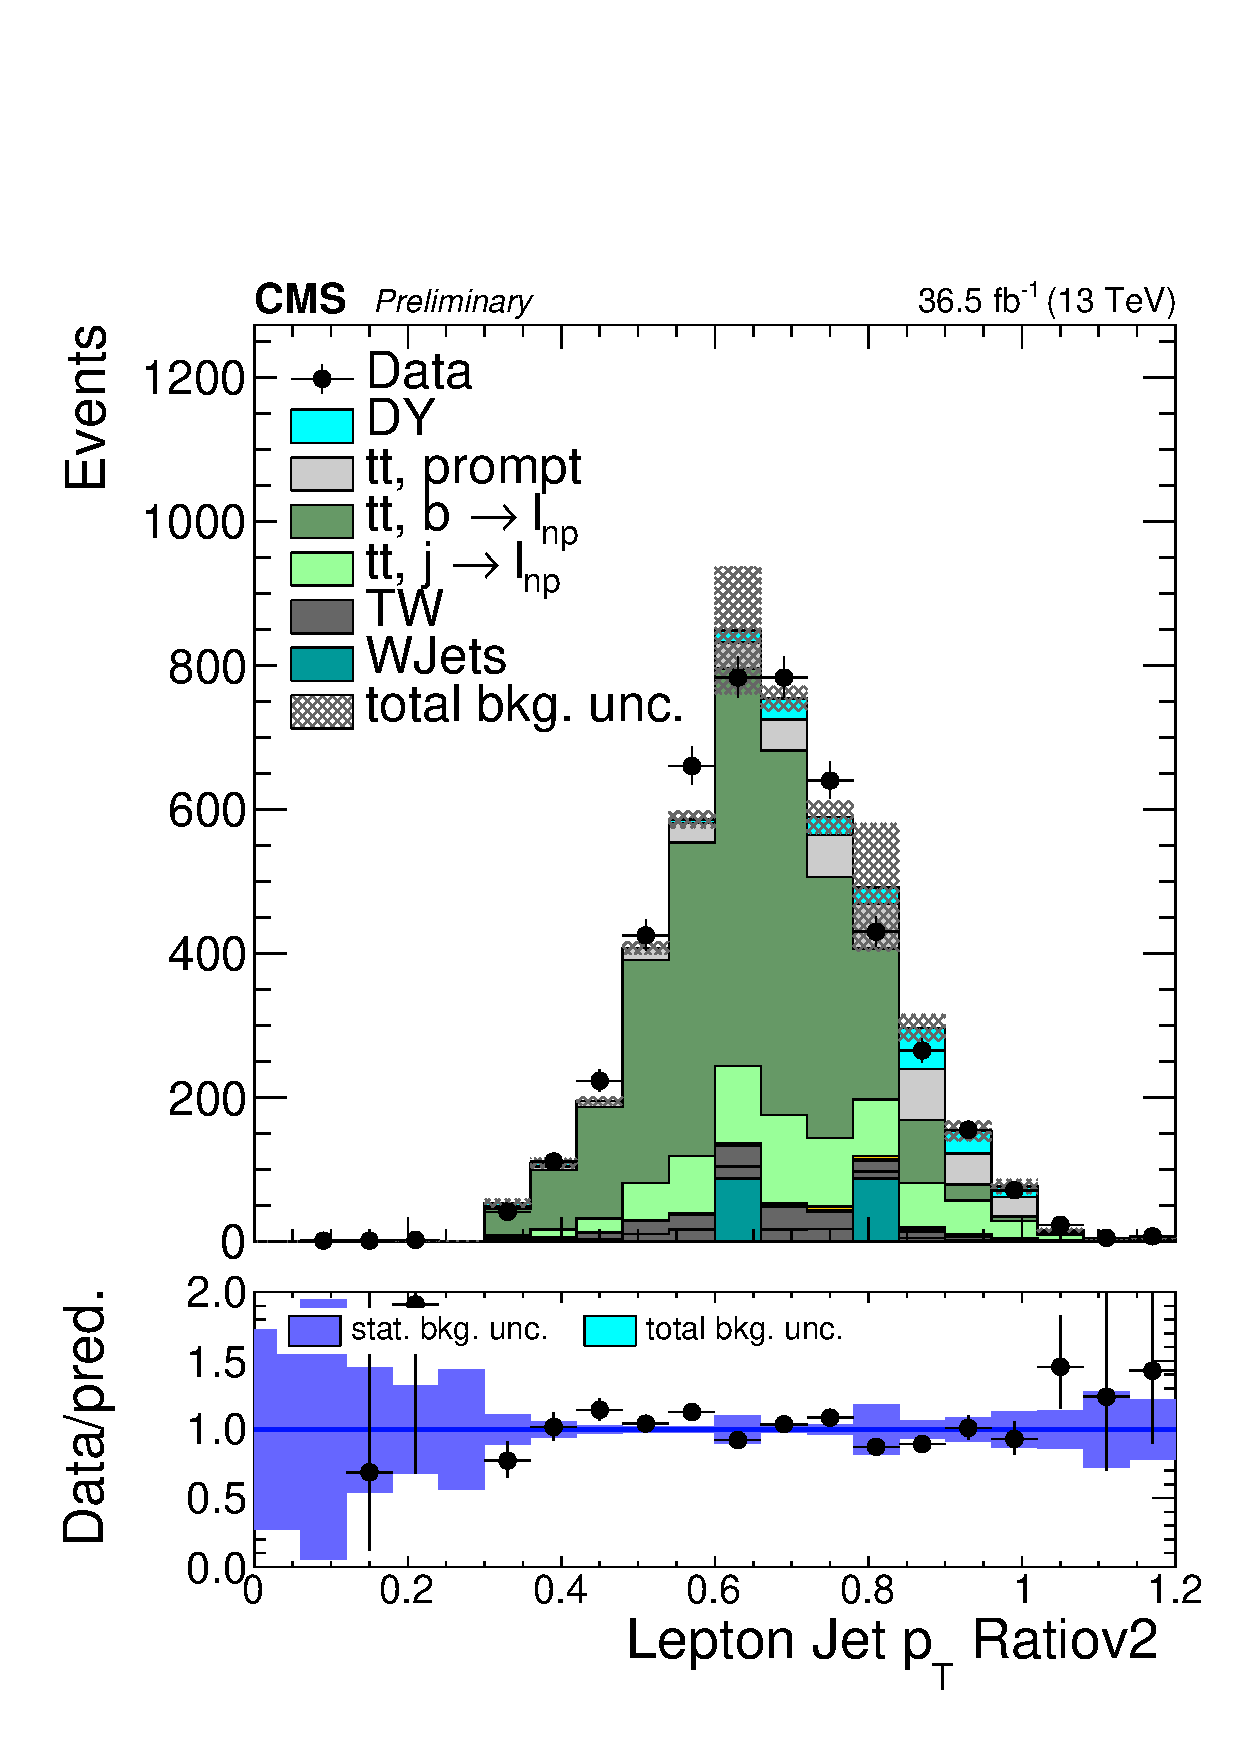
\includegraphics[width=0.32\textwidth]{plots_controlregions/leptons/lep_jetPtRatiov2.pdf}
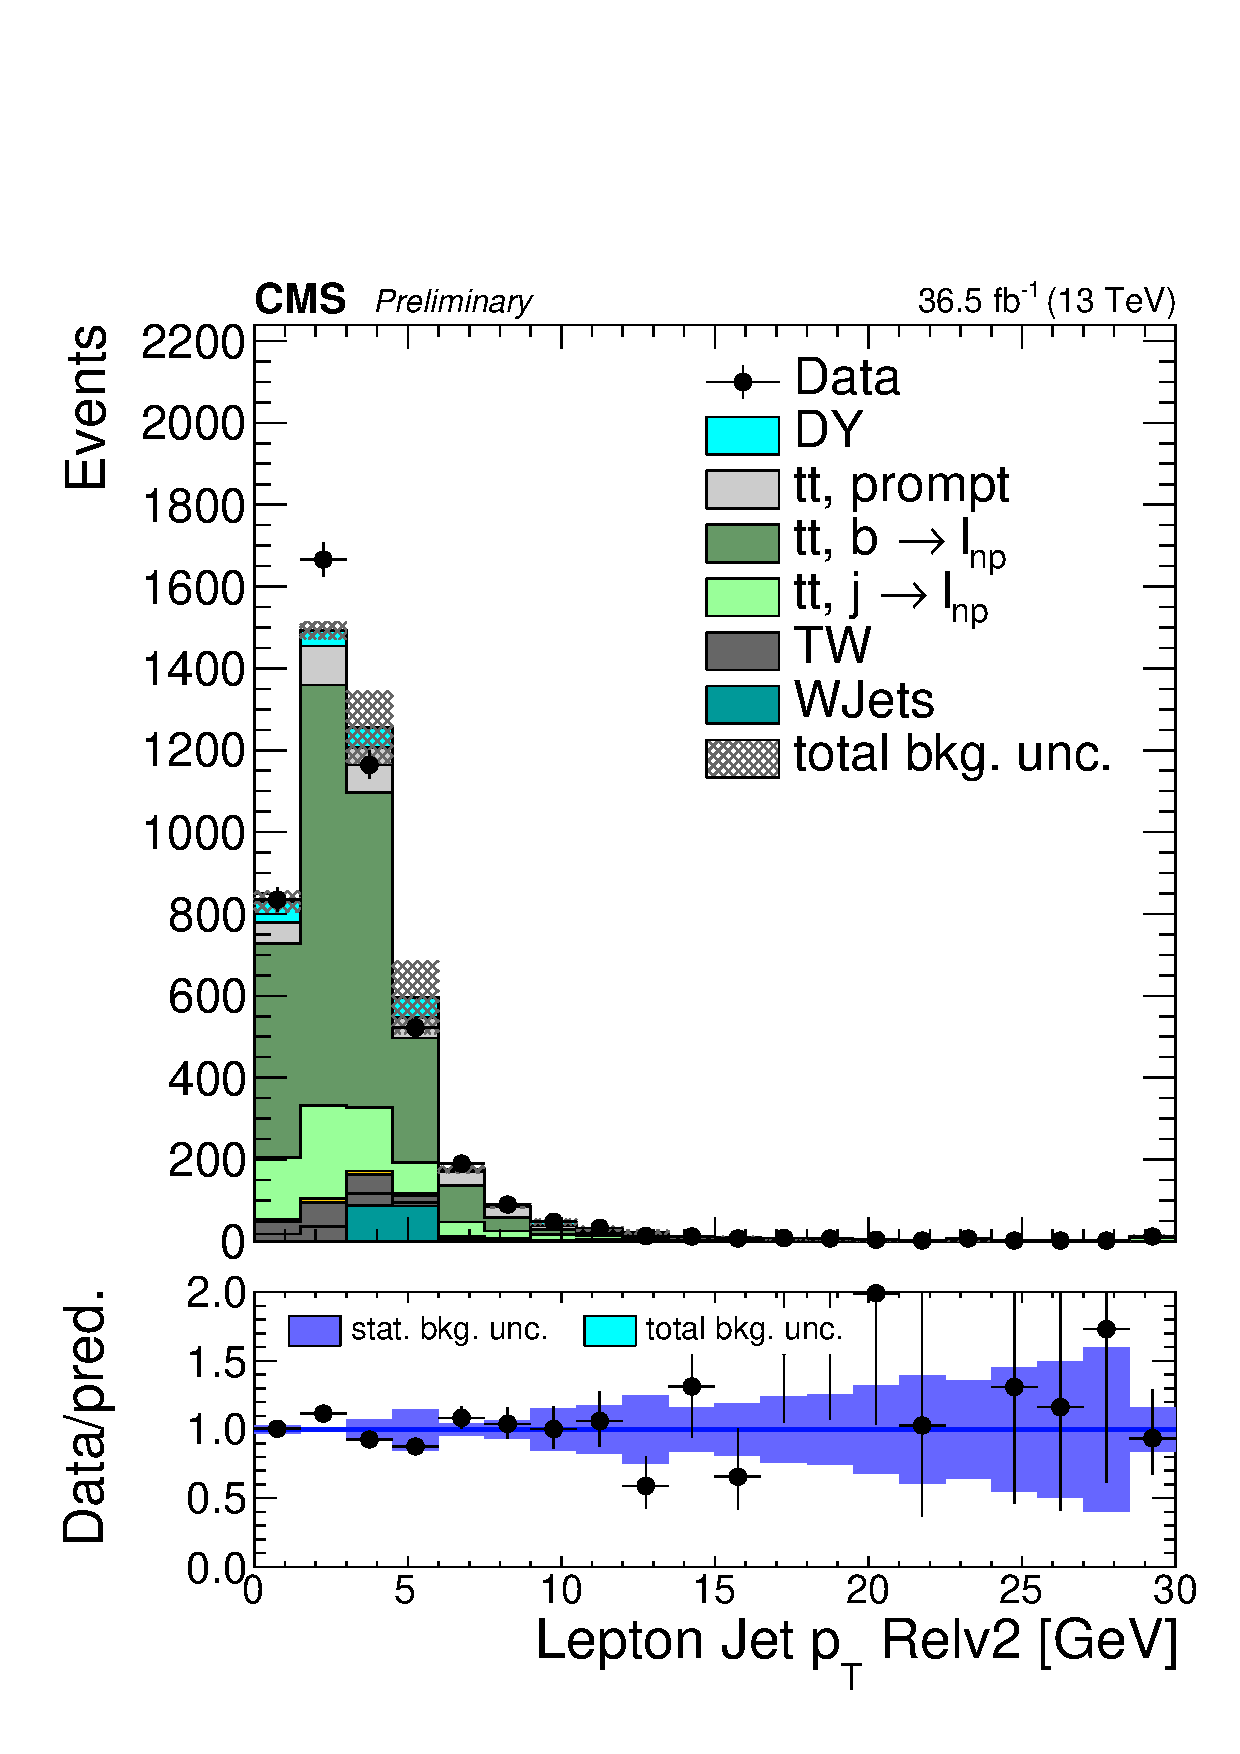
\includegraphics[width=0.32\textwidth]{plots_controlregions/leptons/lep_jetPtRelv2.pdf}
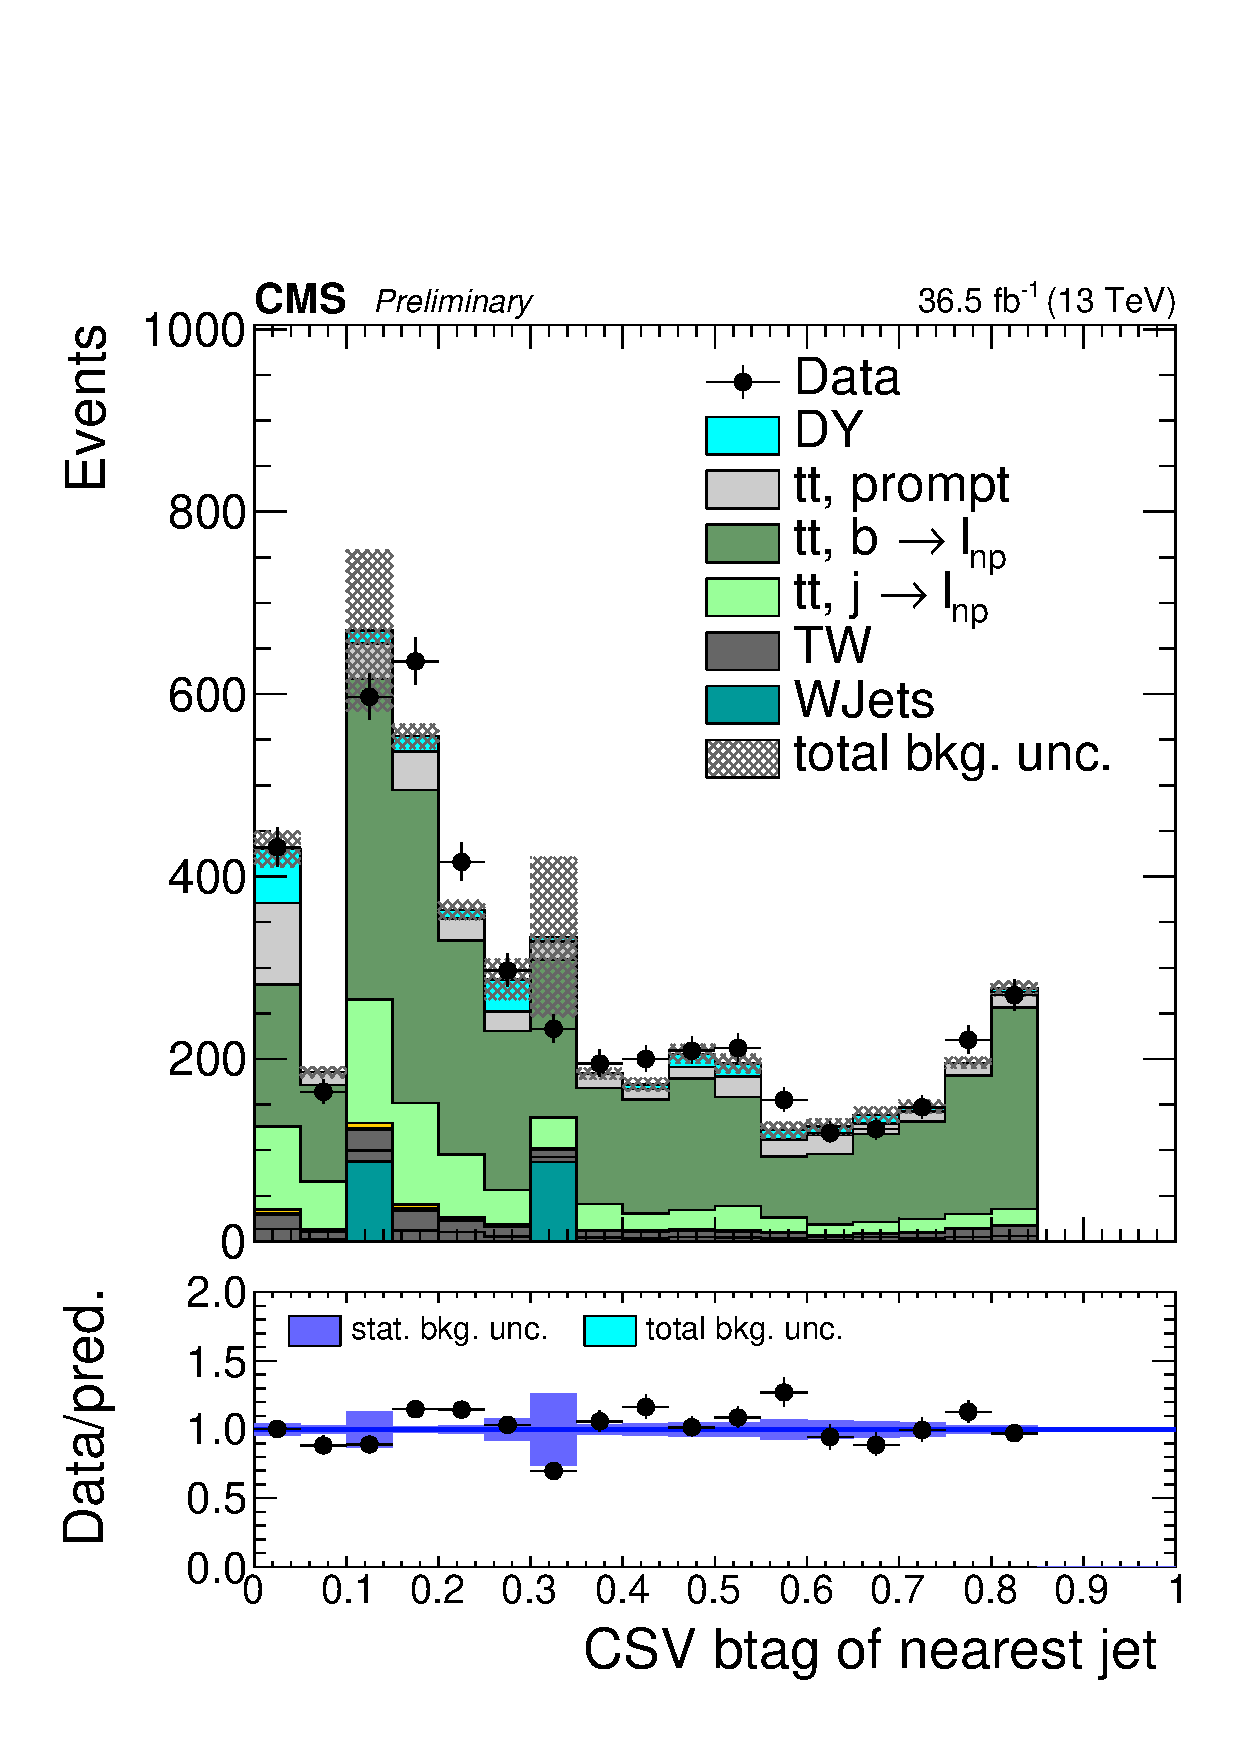
\includegraphics[width=0.32\textwidth]{plots_controlregions/leptons/lep_jetBTagCSV.pdf}\\
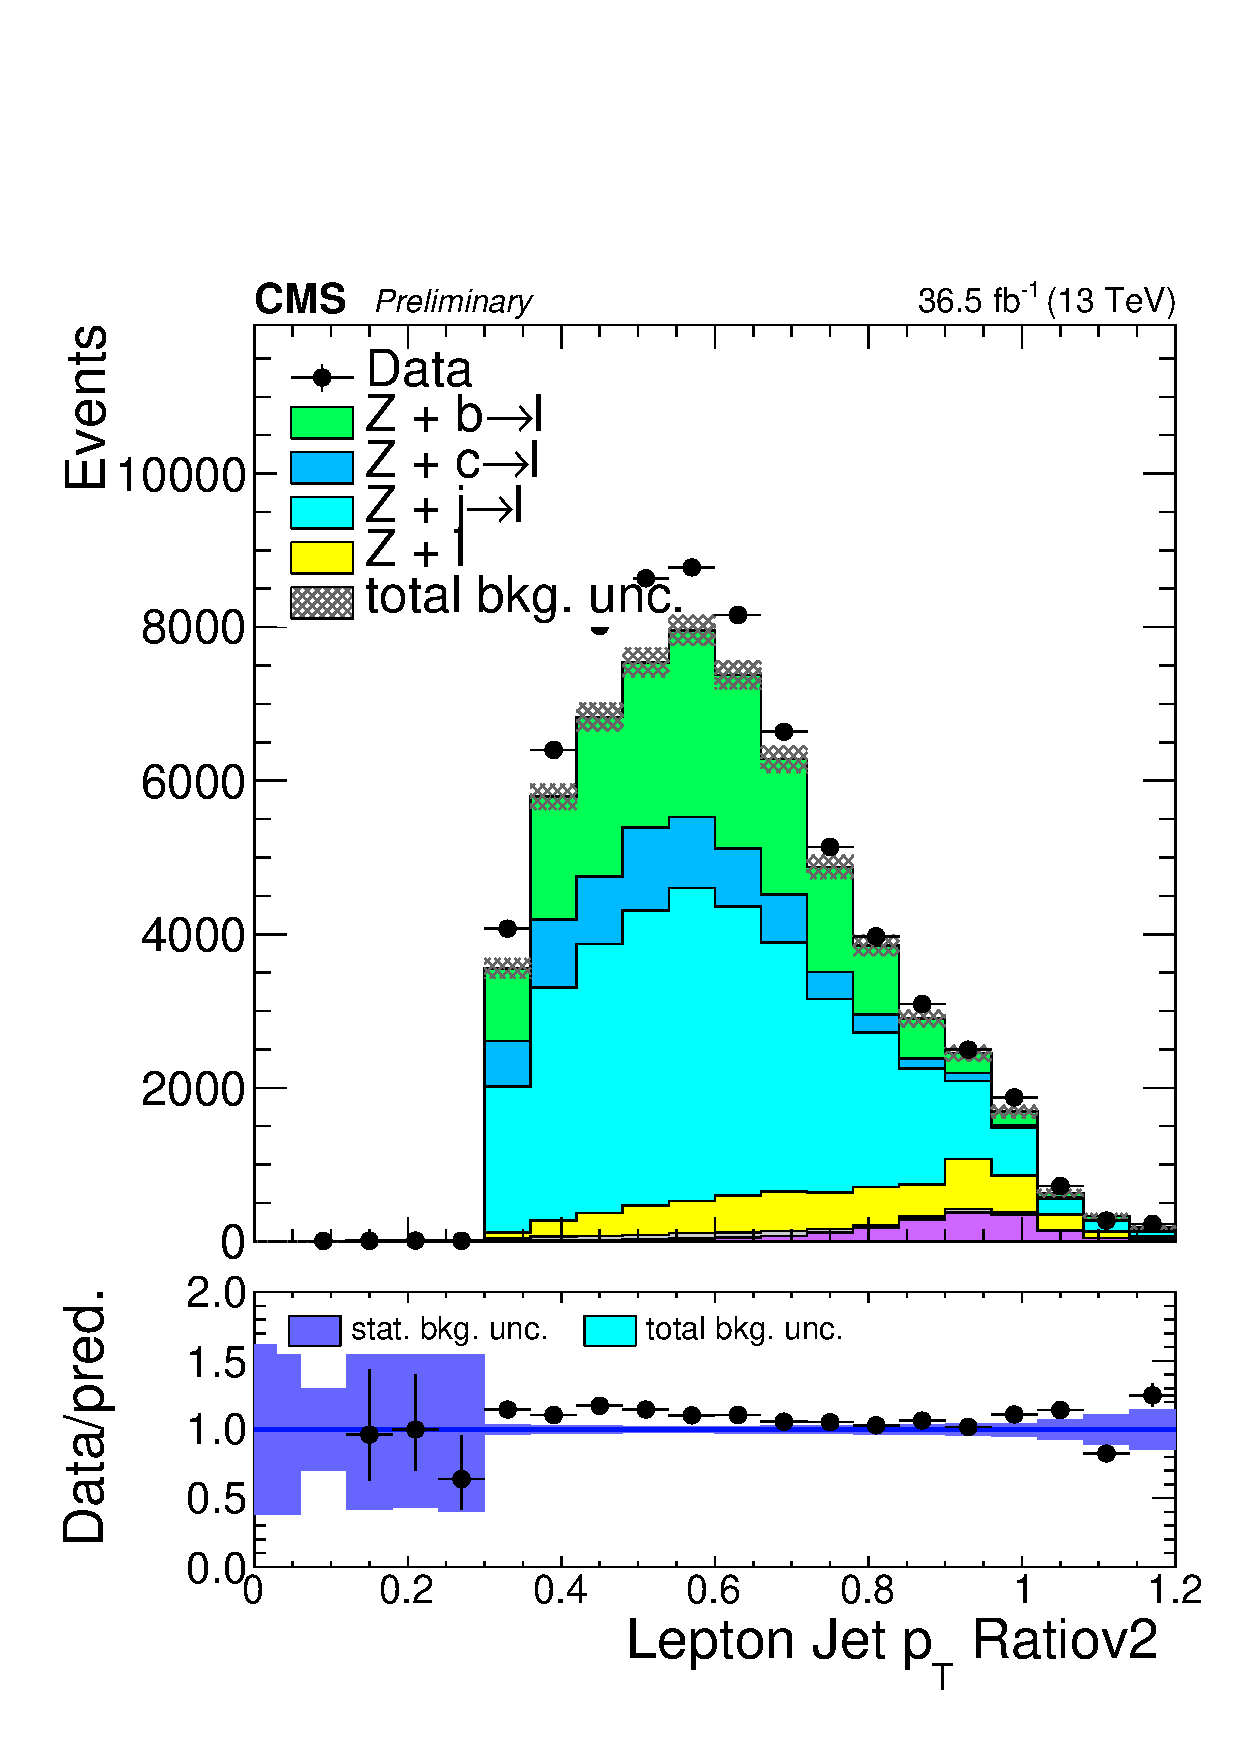
\includegraphics[width=0.32\textwidth]{plots_controlregions/leptons/lep_jetPtRatiov2_Zl.pdf}
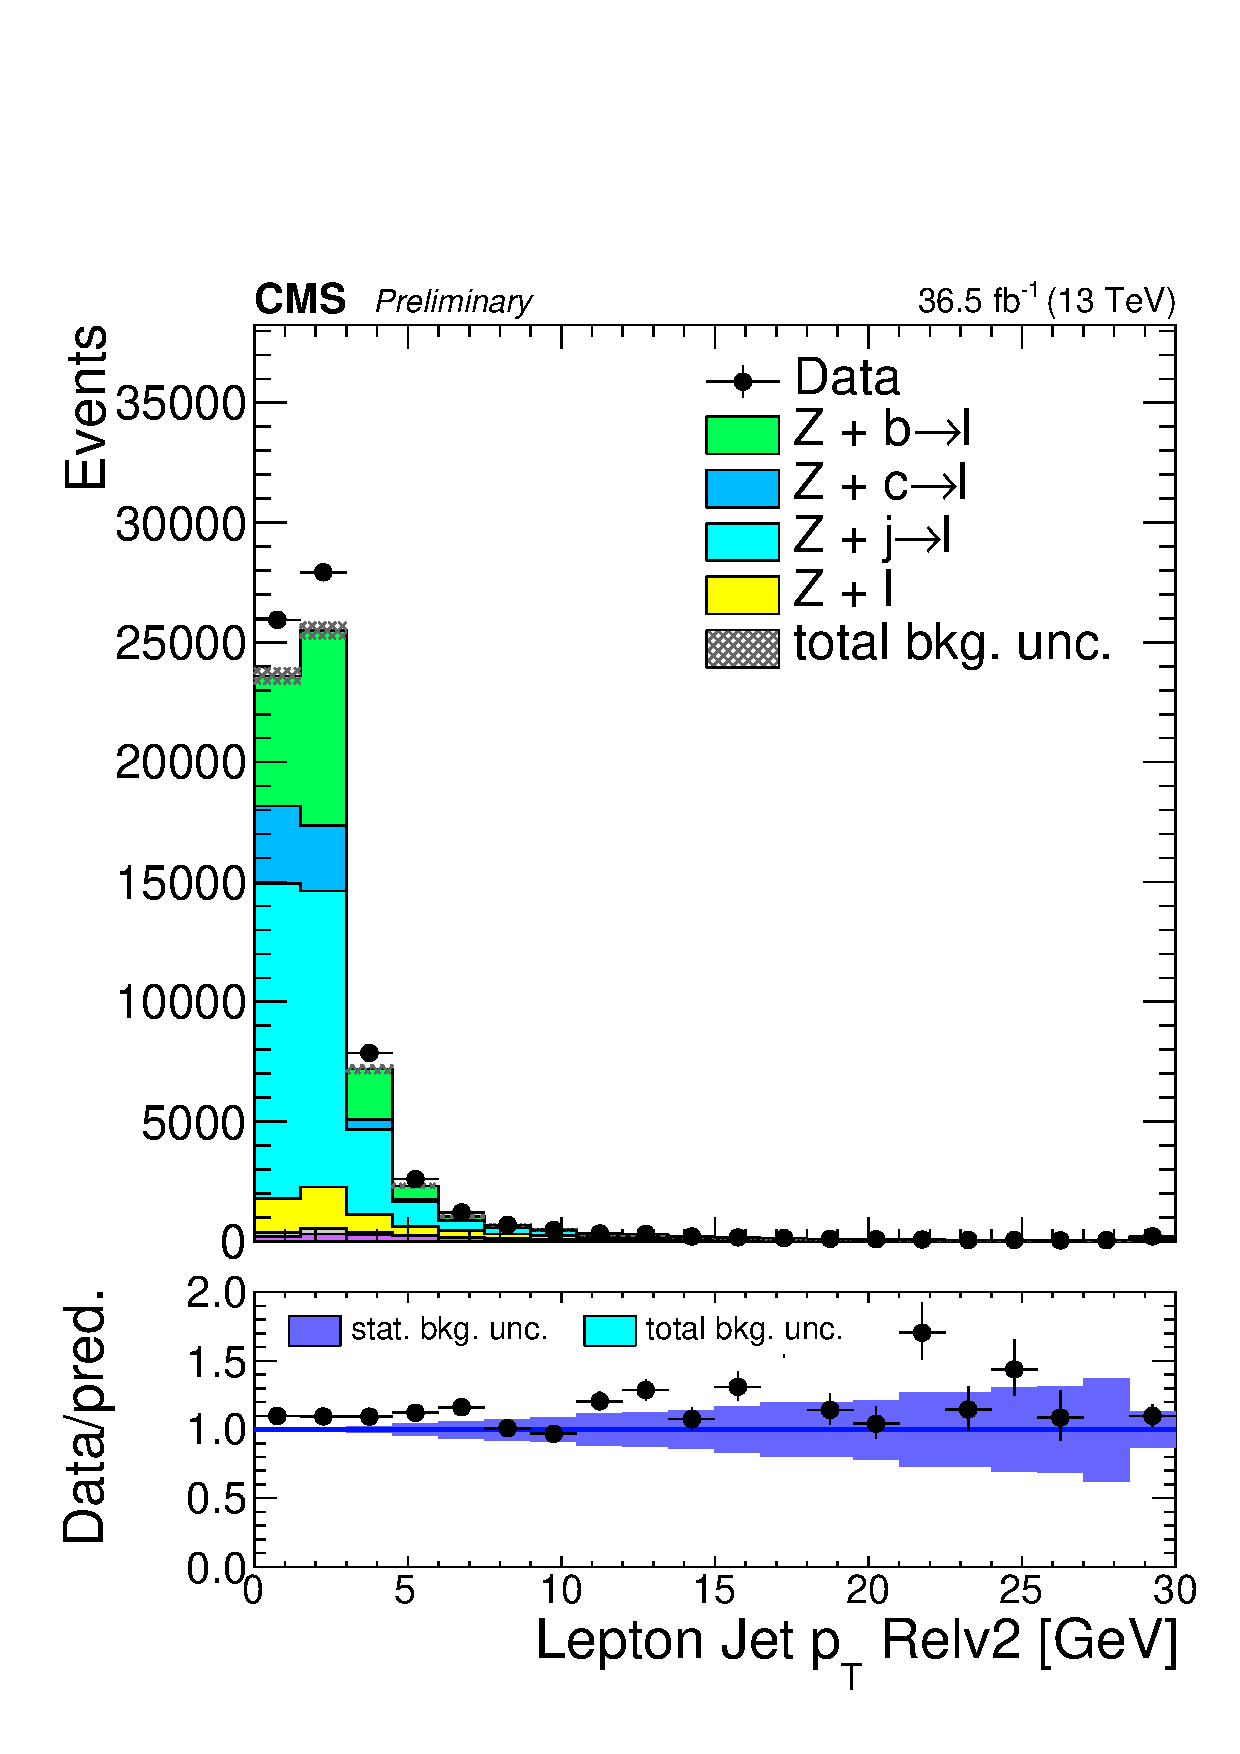
\includegraphics[width=0.32\textwidth]{plots_controlregions/leptons/lep_jetPtRelv2_Zl.pdf}
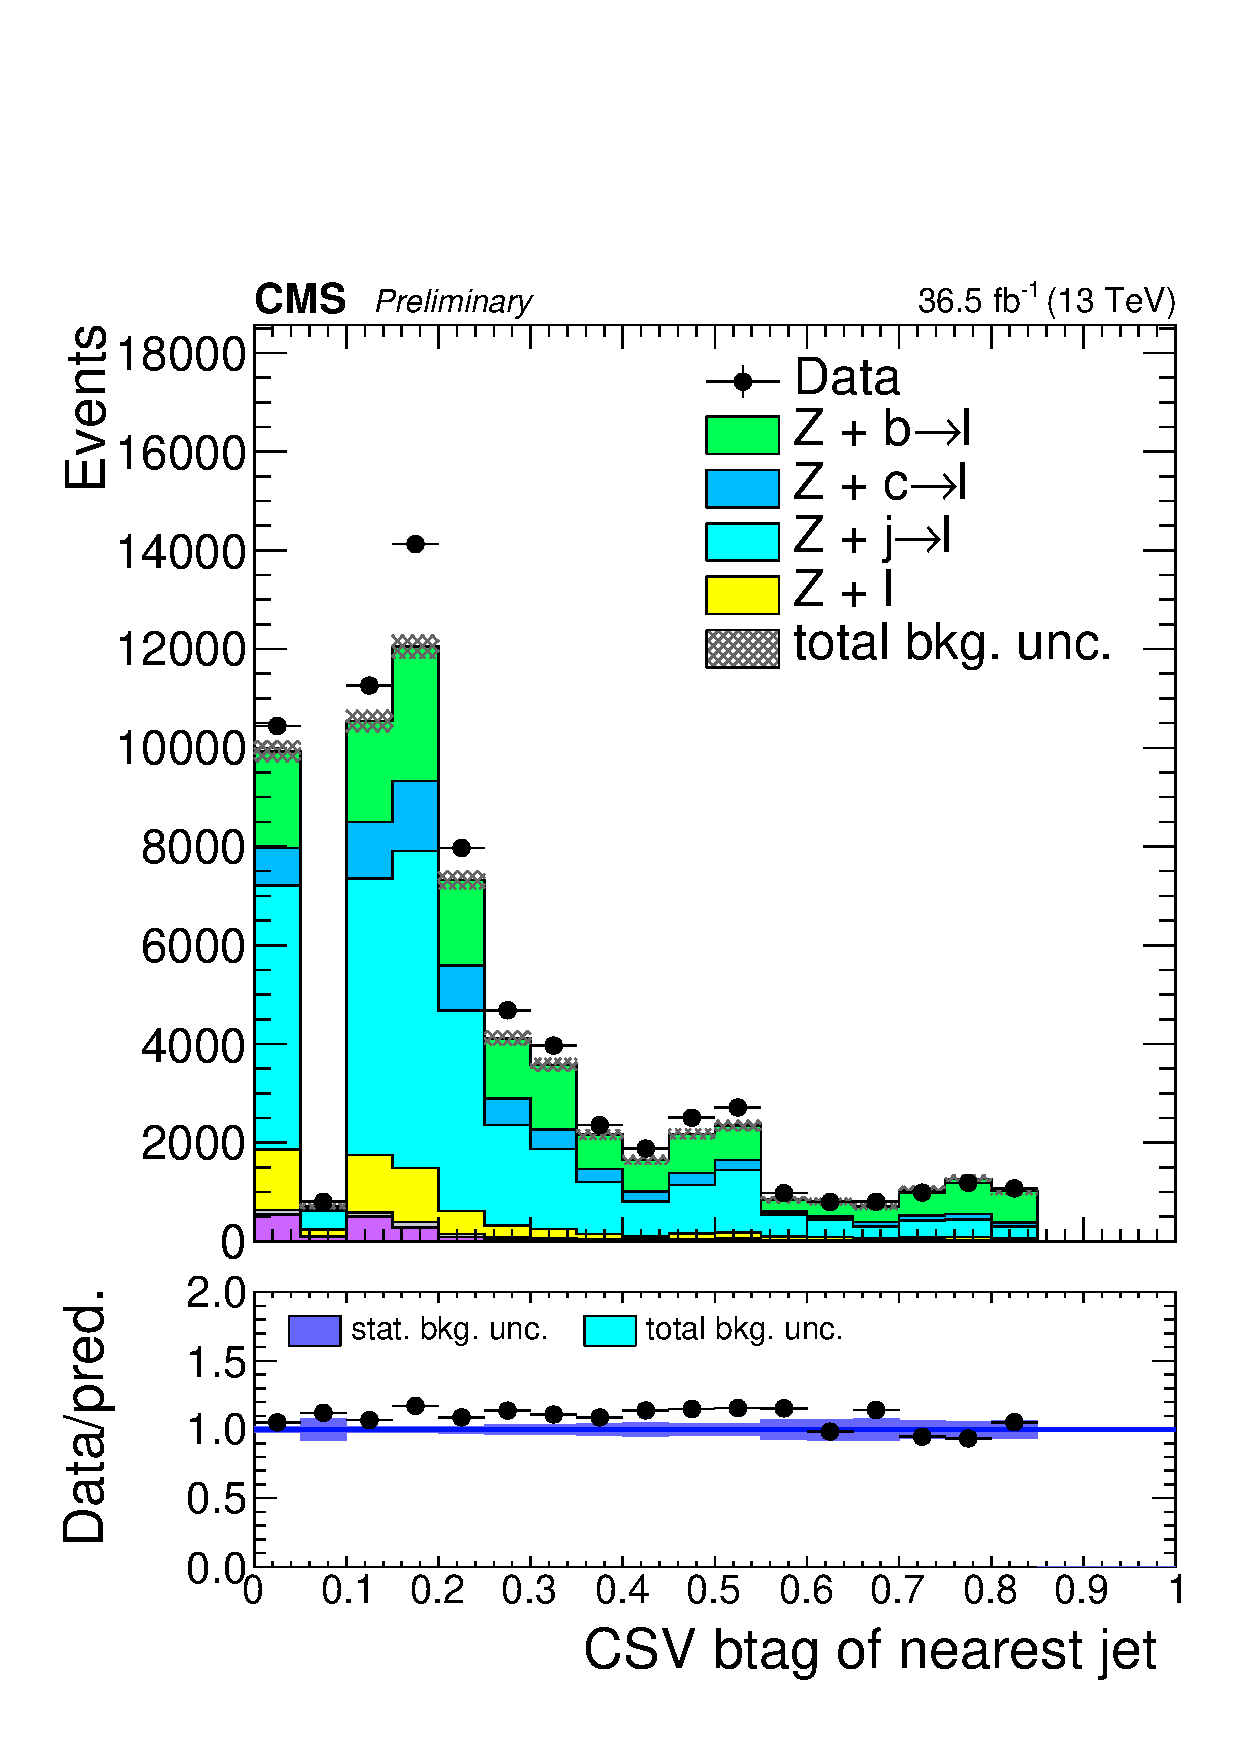
\includegraphics[width=0.32\textwidth]{plots_controlregions/leptons/lep_jetBTagCSV_Zl.pdf}
        \caption{Comparison of the distributions for the lepton $\ptRatio$ (left), $\ptRel$ (center) and the b-tagging discriminator of the associated jet (right),  between data and simulations in control regions enriched in prompt leptons (top), non-prompt leptons (center), and Z+jets events (bottom) , as described in the text. The uncertainty shown on the simulation is only statistical.}
        \label{fig:lep-distributions-2}
\end{figure}

\begin{figure}
        \centering
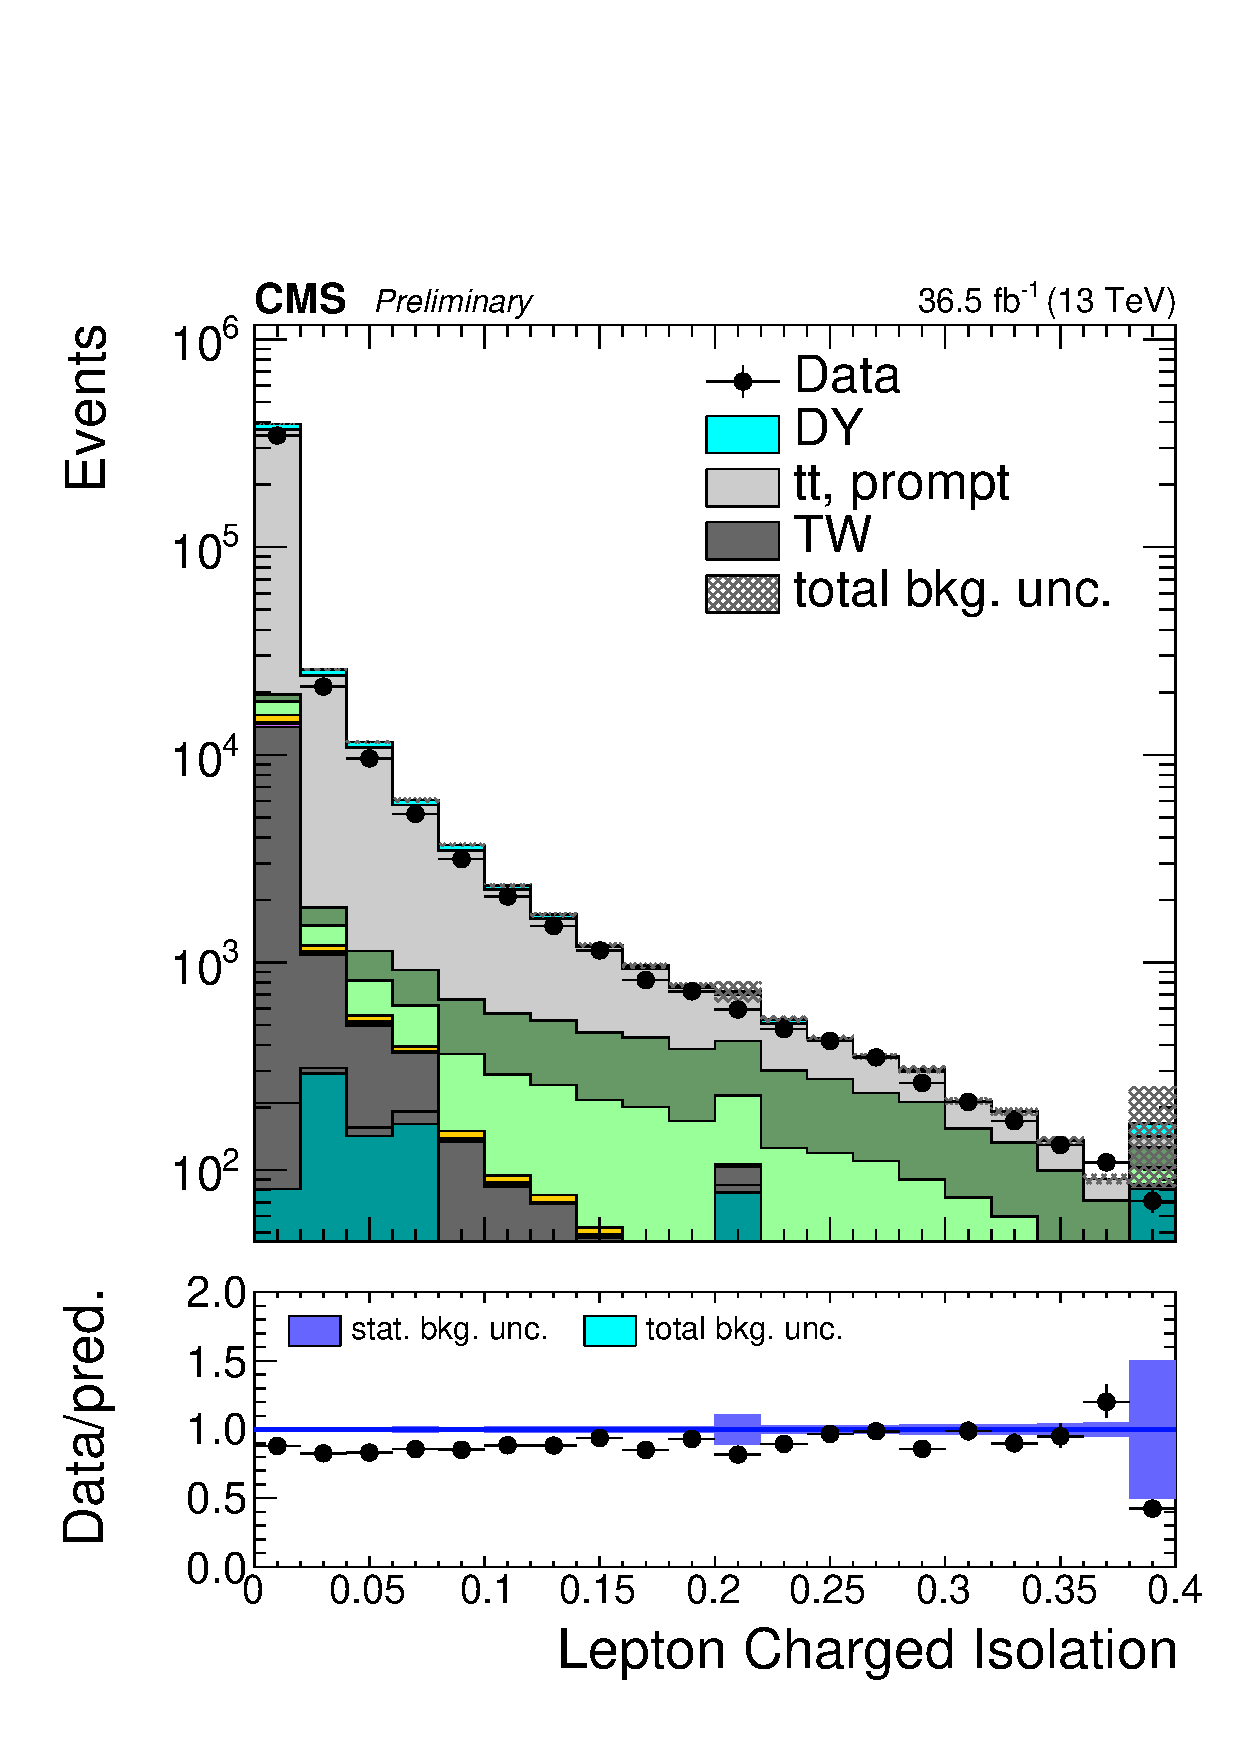
\includegraphics[width=0.32\textwidth]{plots_controlregions/leptons/ttbar/lep_miniRelIsoCharged_log.pdf}
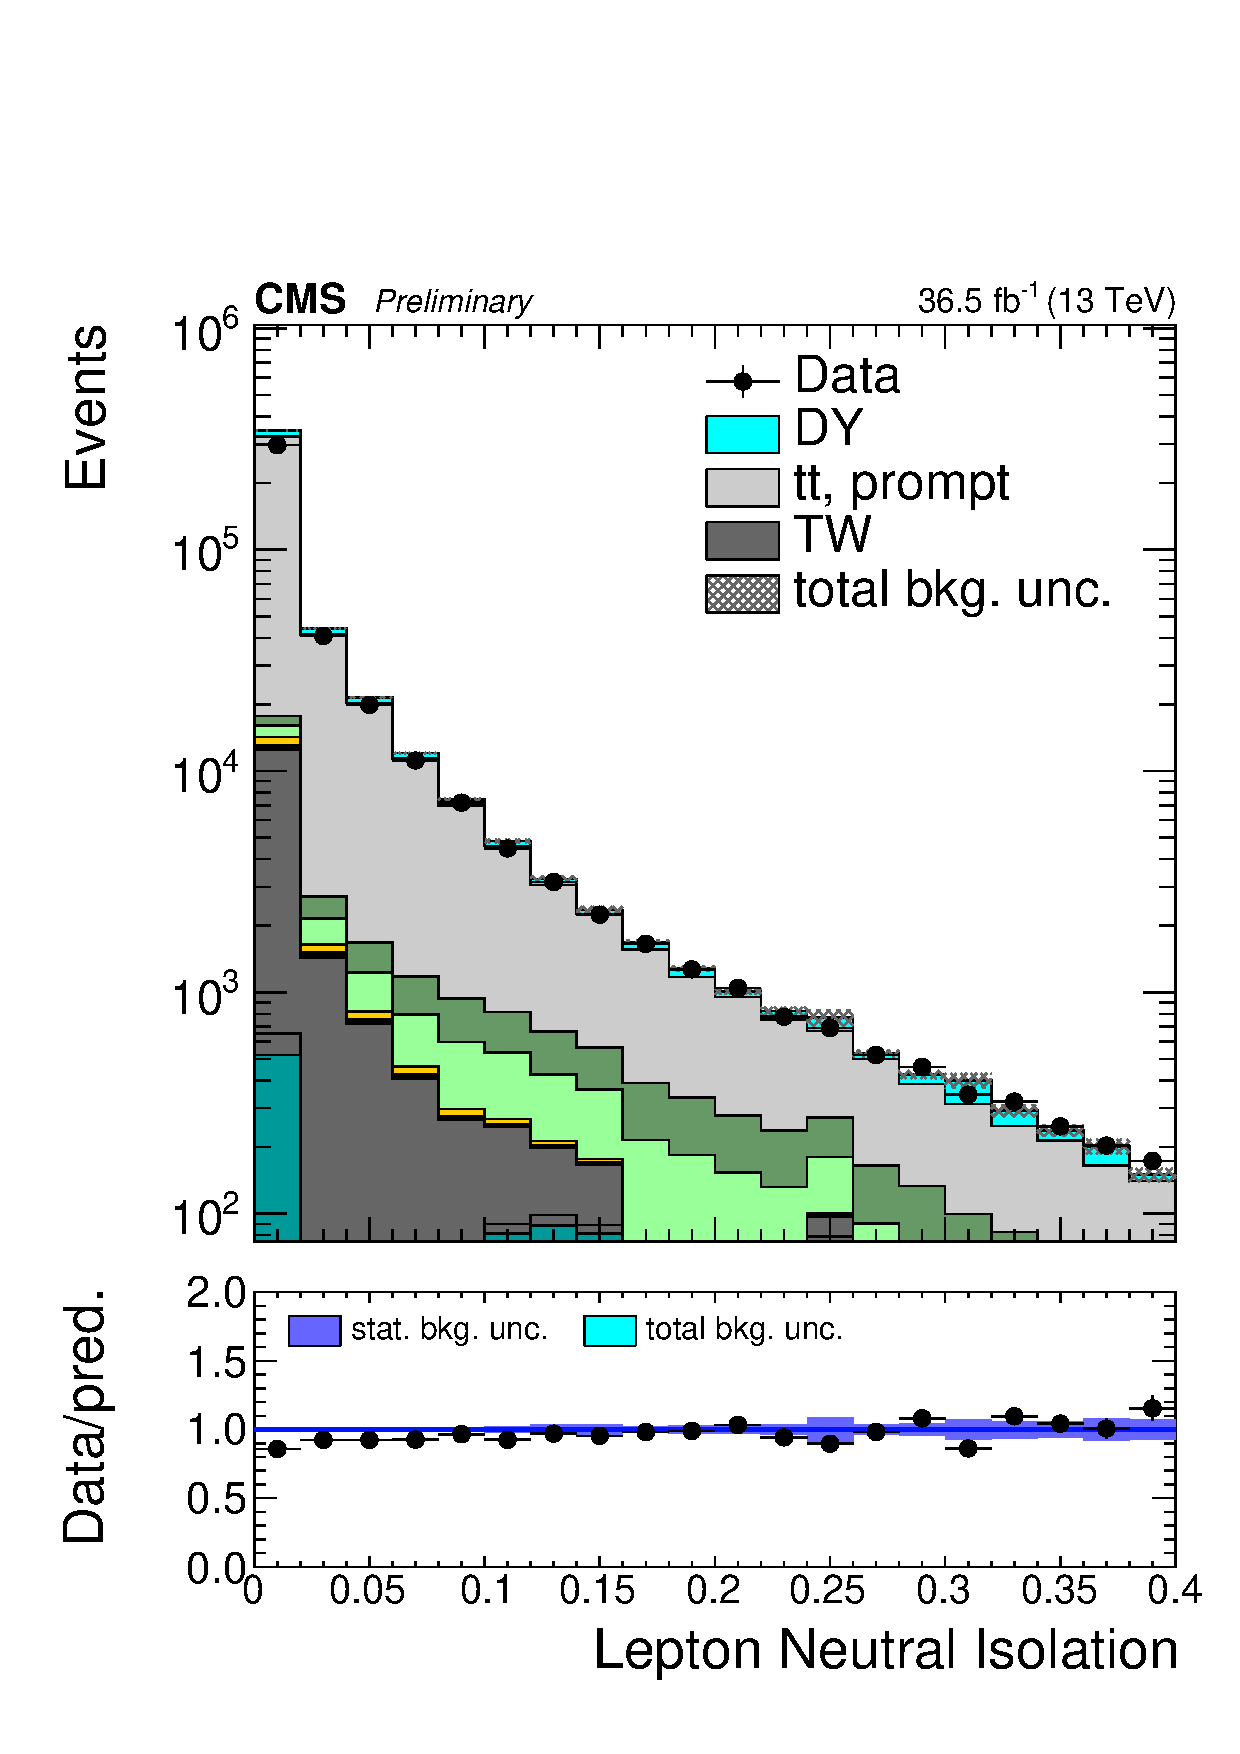
\includegraphics[width=0.32\textwidth]{plots_controlregions/leptons/ttbar/lep_miniRelIsoNeutral_log.pdf}
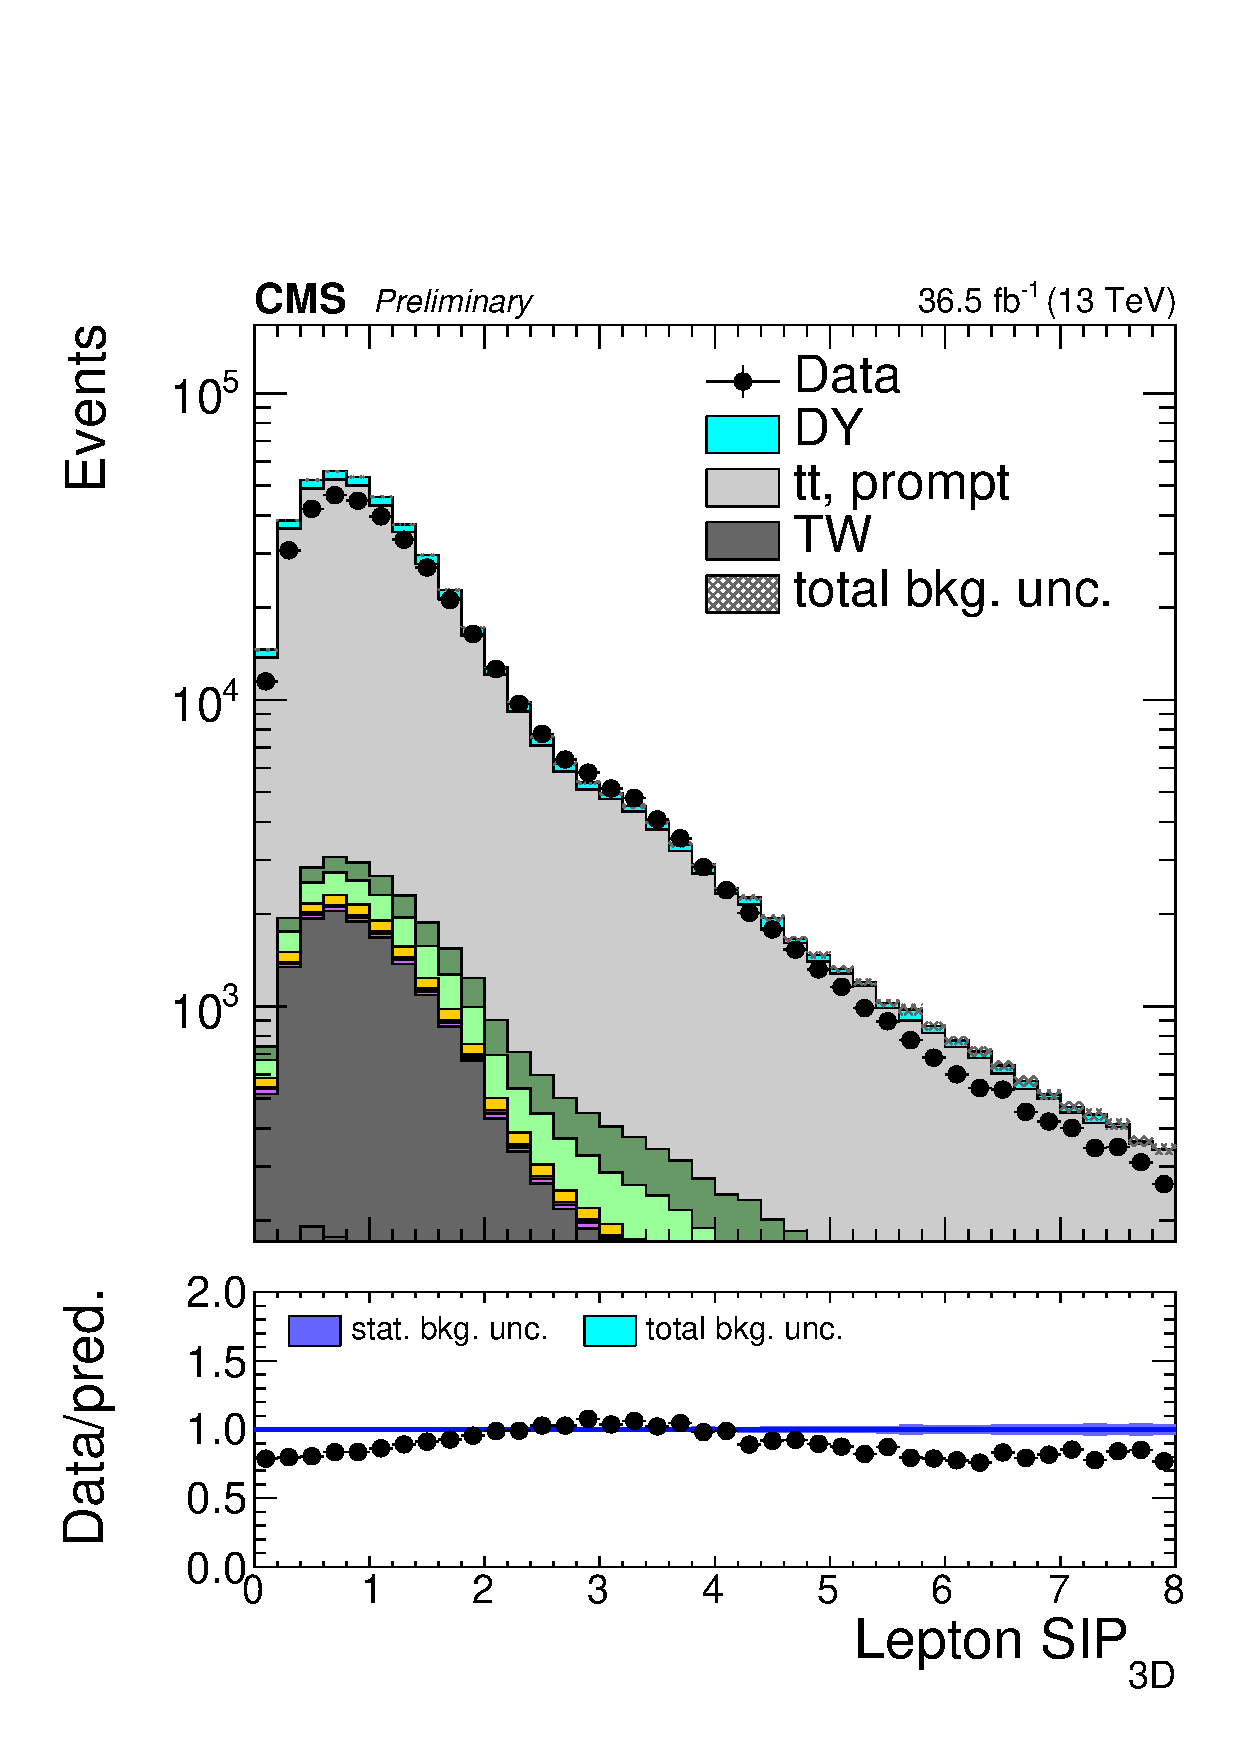
\includegraphics[width=0.32\textwidth]{plots_controlregions/leptons/ttbar/lep_sip3d_log.pdf}\\
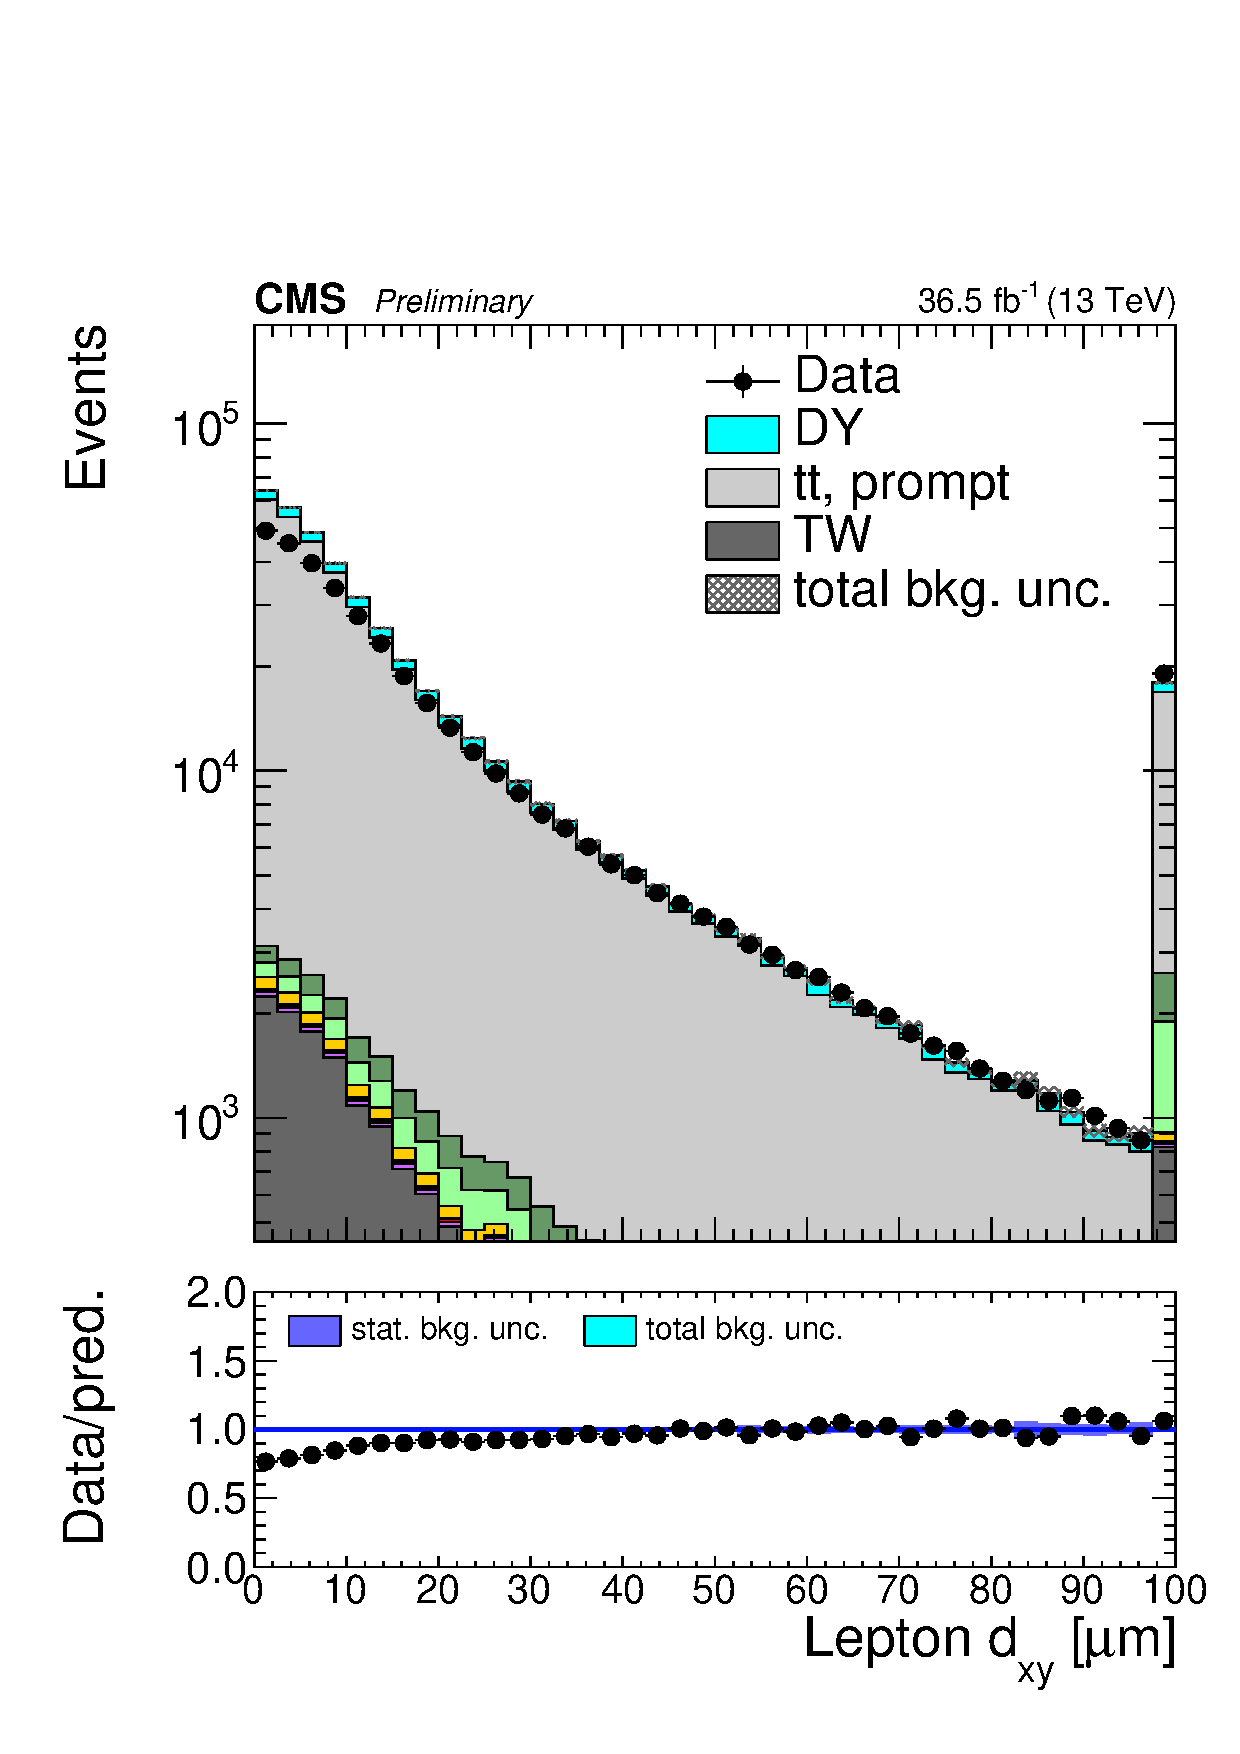
\includegraphics[width=0.32\textwidth]{plots_controlregions/leptons/ttbar/lep_dxy_log.pdf}
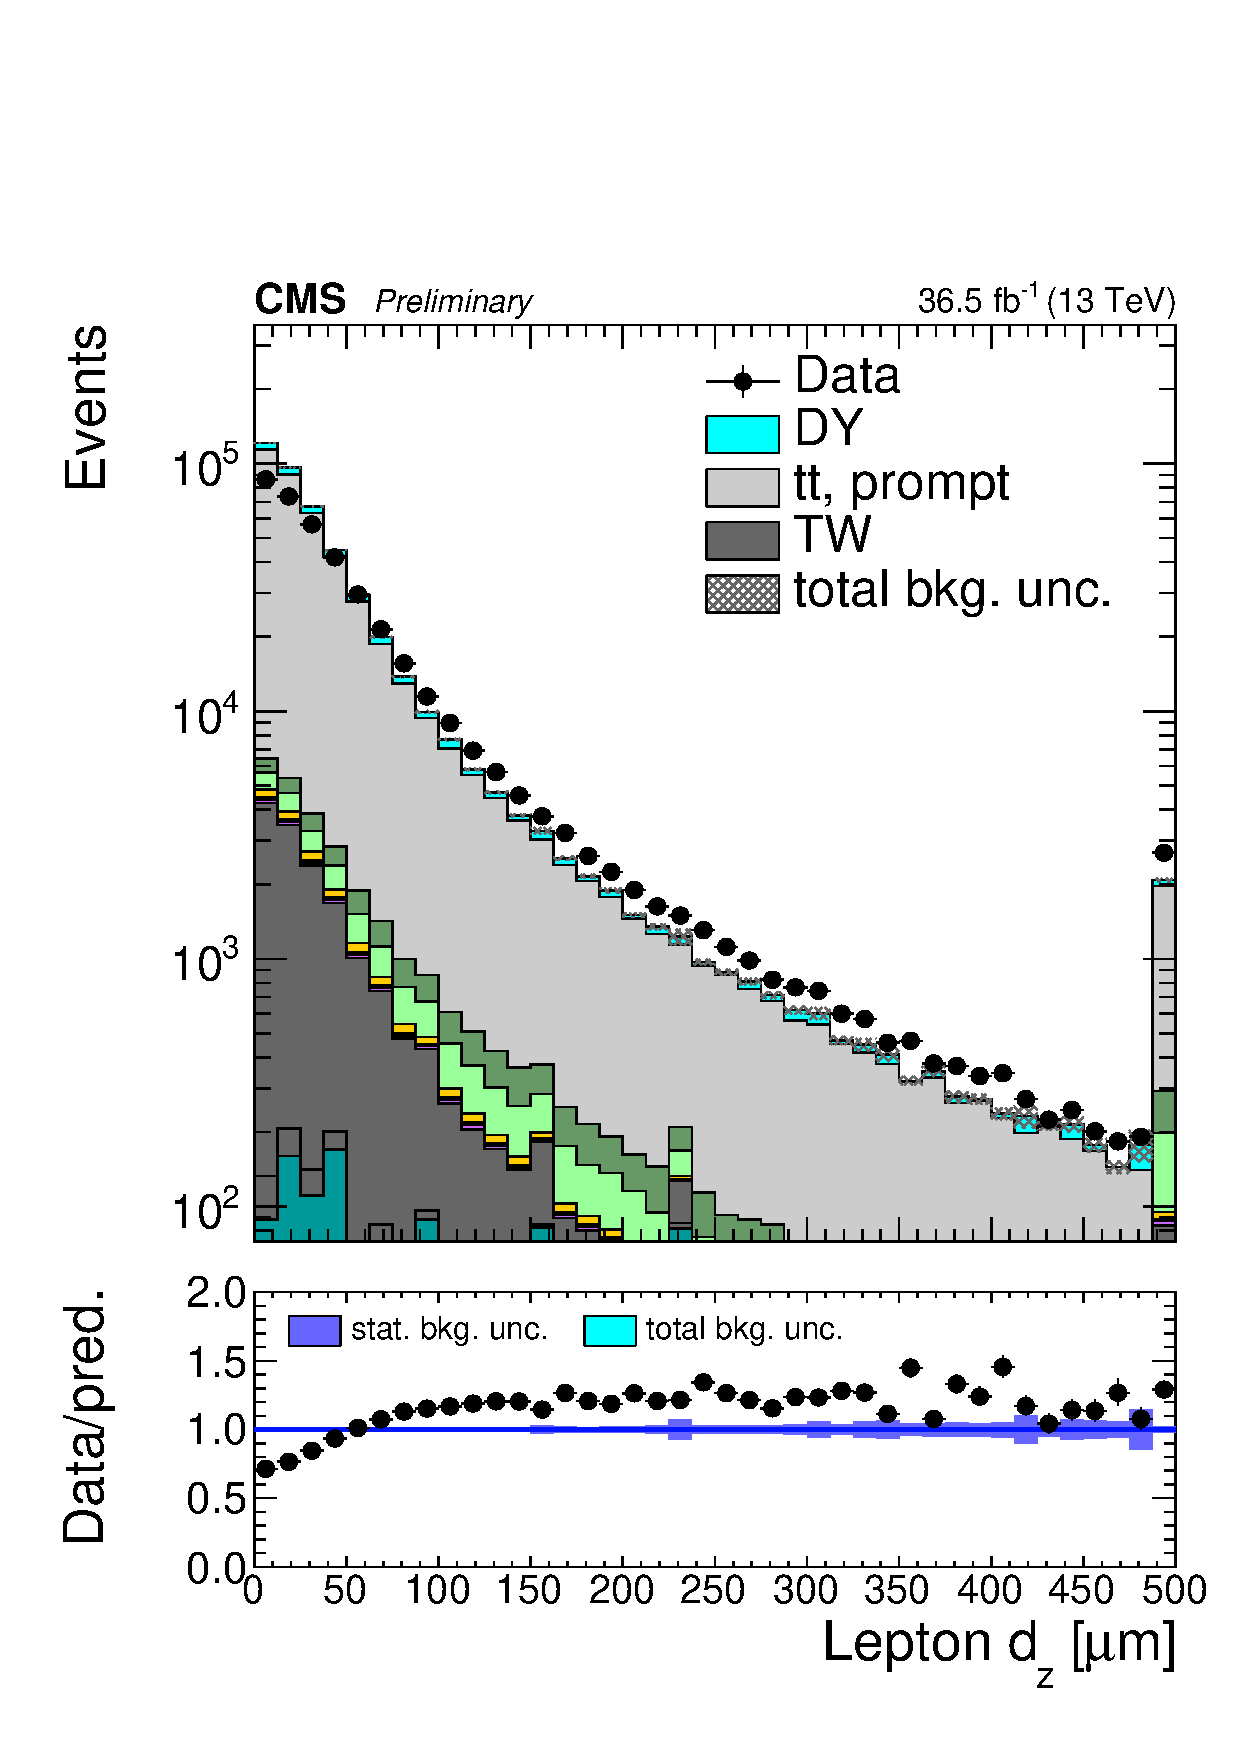
\includegraphics[width=0.32\textwidth]{plots_controlregions/leptons/ttbar/lep_dz_log.pdf}
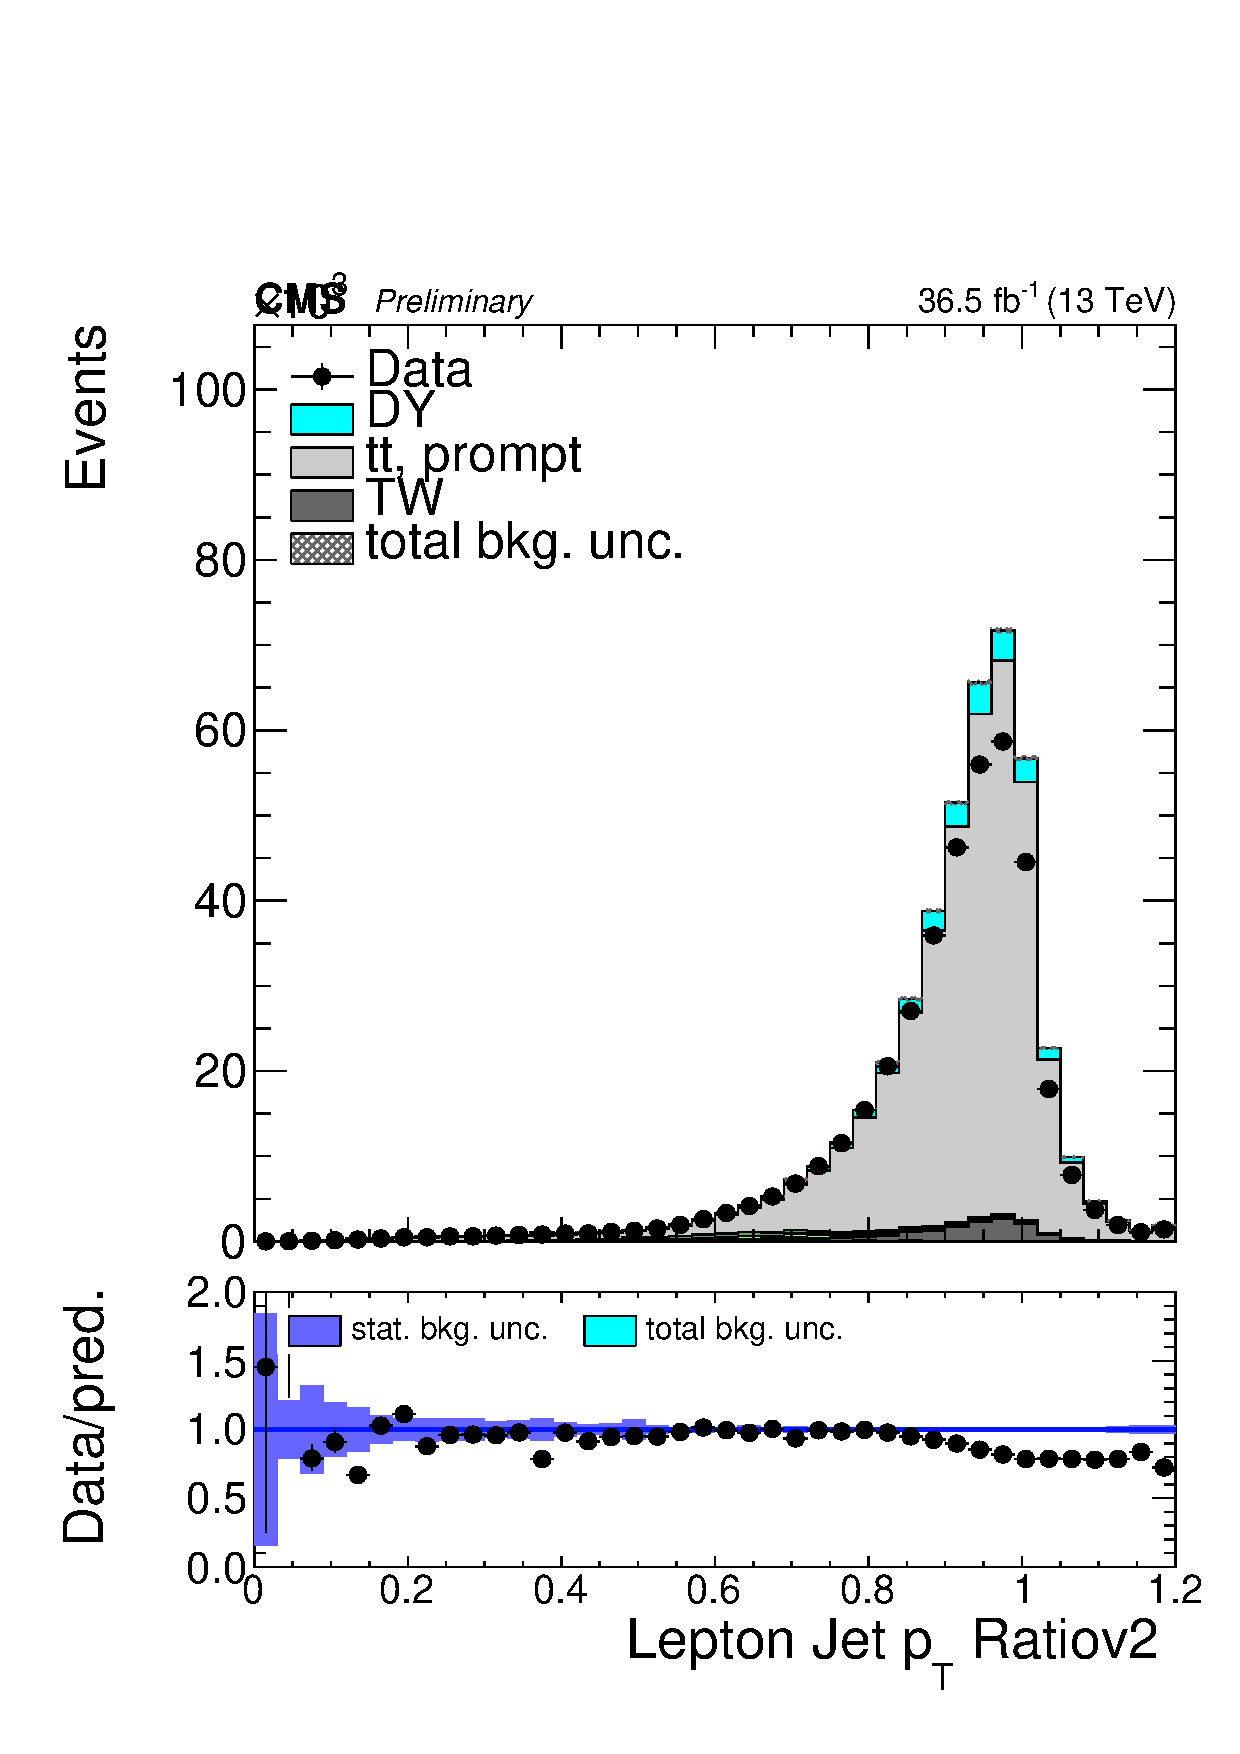
\includegraphics[width=0.32\textwidth]{plots_controlregions/leptons/ttbar/lep_jetPtRatiov2.pdf}
        \caption{Summary of the input variables to the lepton MVA in a ttbar enriched sample, in data and simulation. The uncertainty shown on the simulation is only statistical.}
        \label{fig:lep-distributions-3}
\end{figure}

\begin{figure}
        \centering
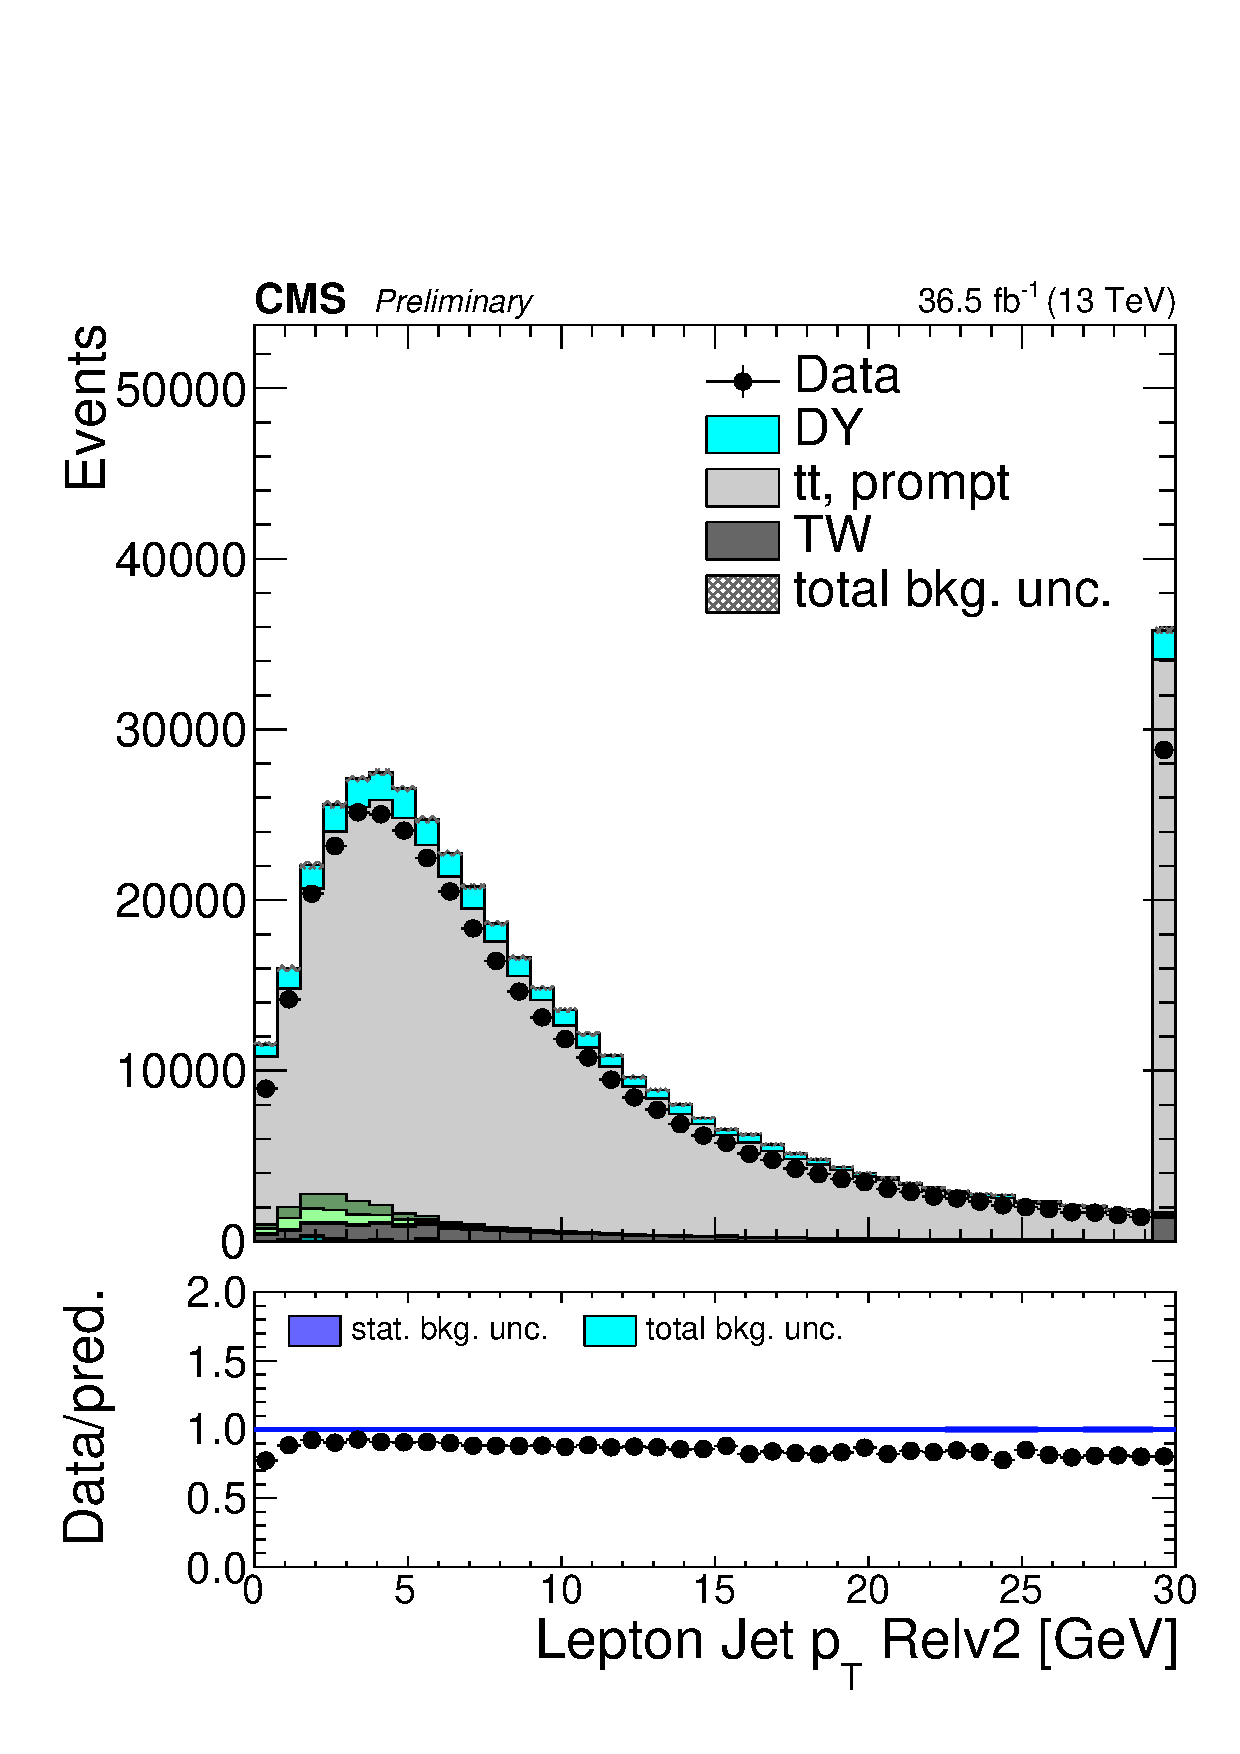
\includegraphics[width=0.32\textwidth]{plots_controlregions/leptons/ttbar/lep_jetPtRelv2.pdf}
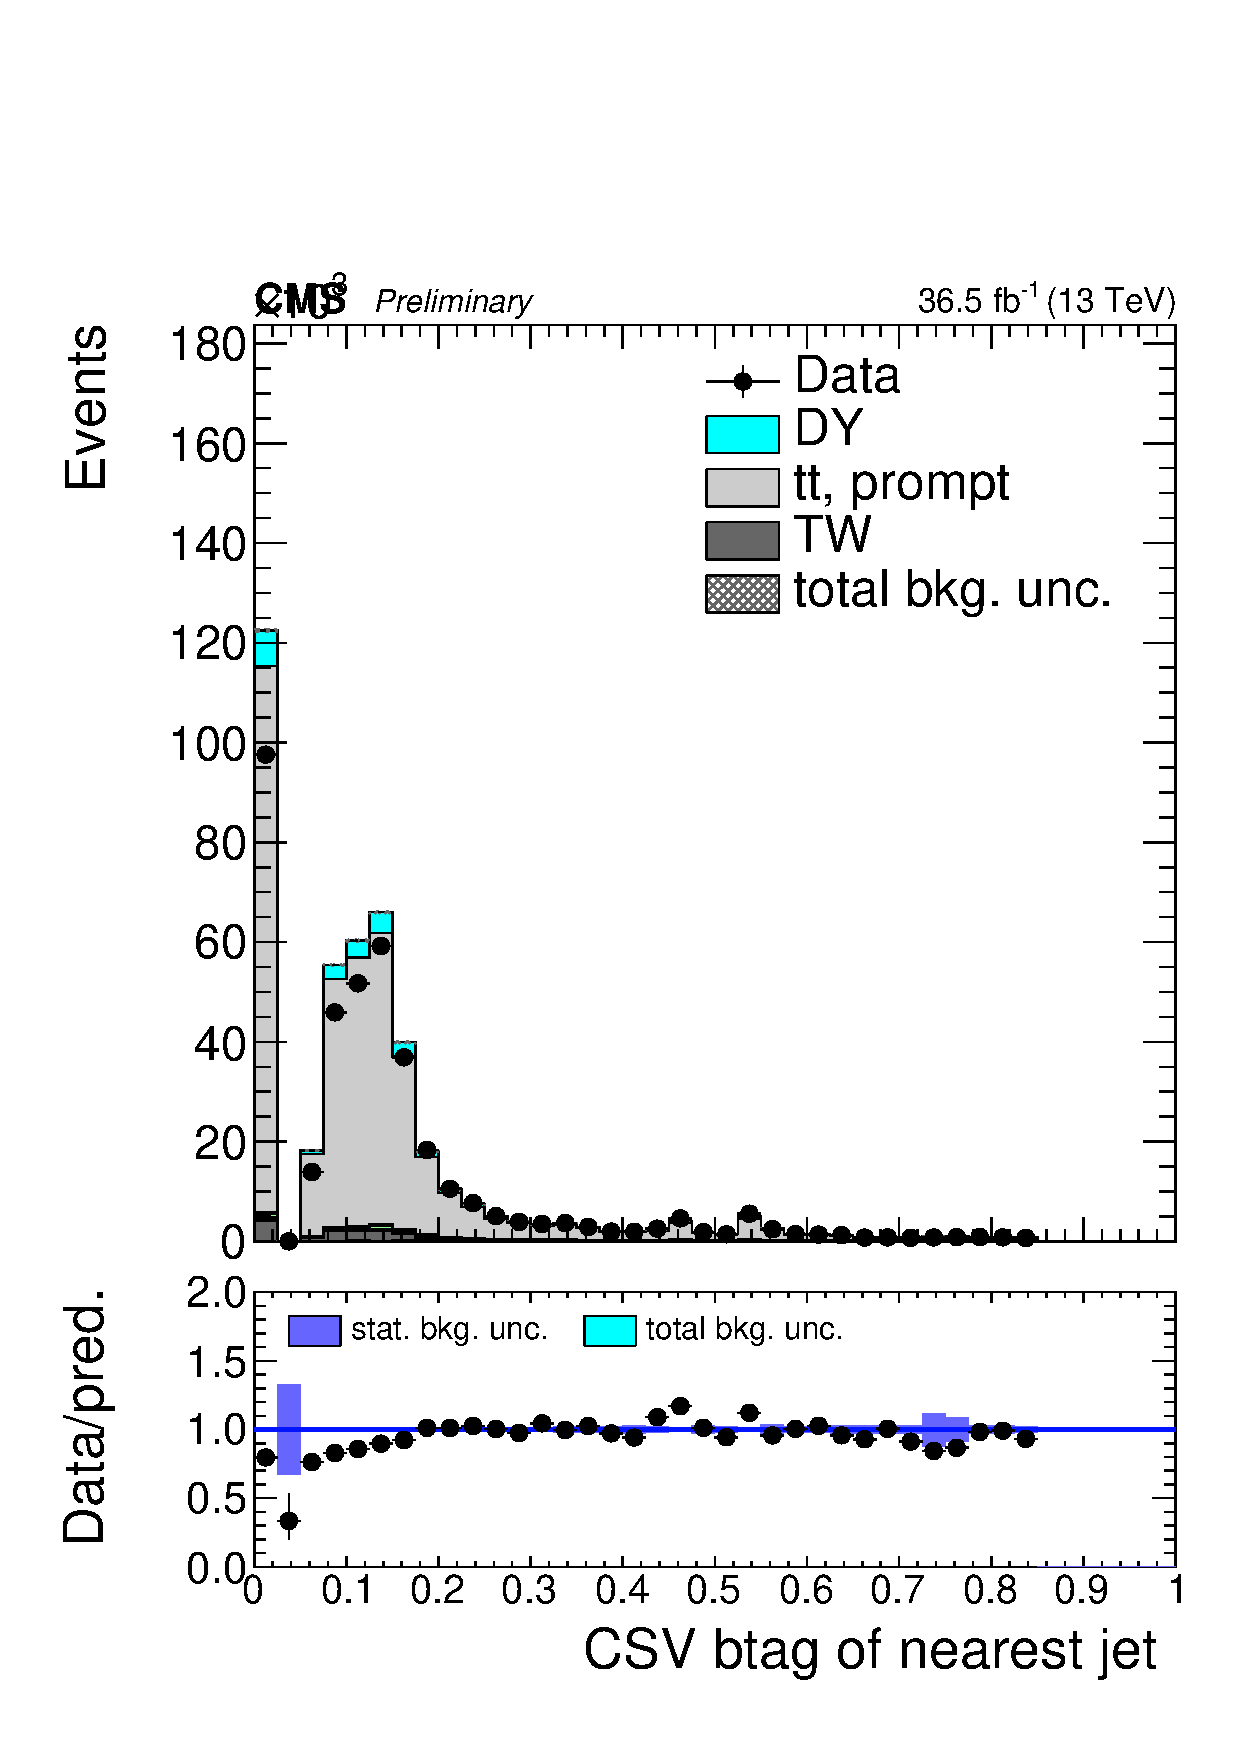
\includegraphics[width=0.32\textwidth]{plots_controlregions/leptons/ttbar/lep_jetBTagCSV.pdf}
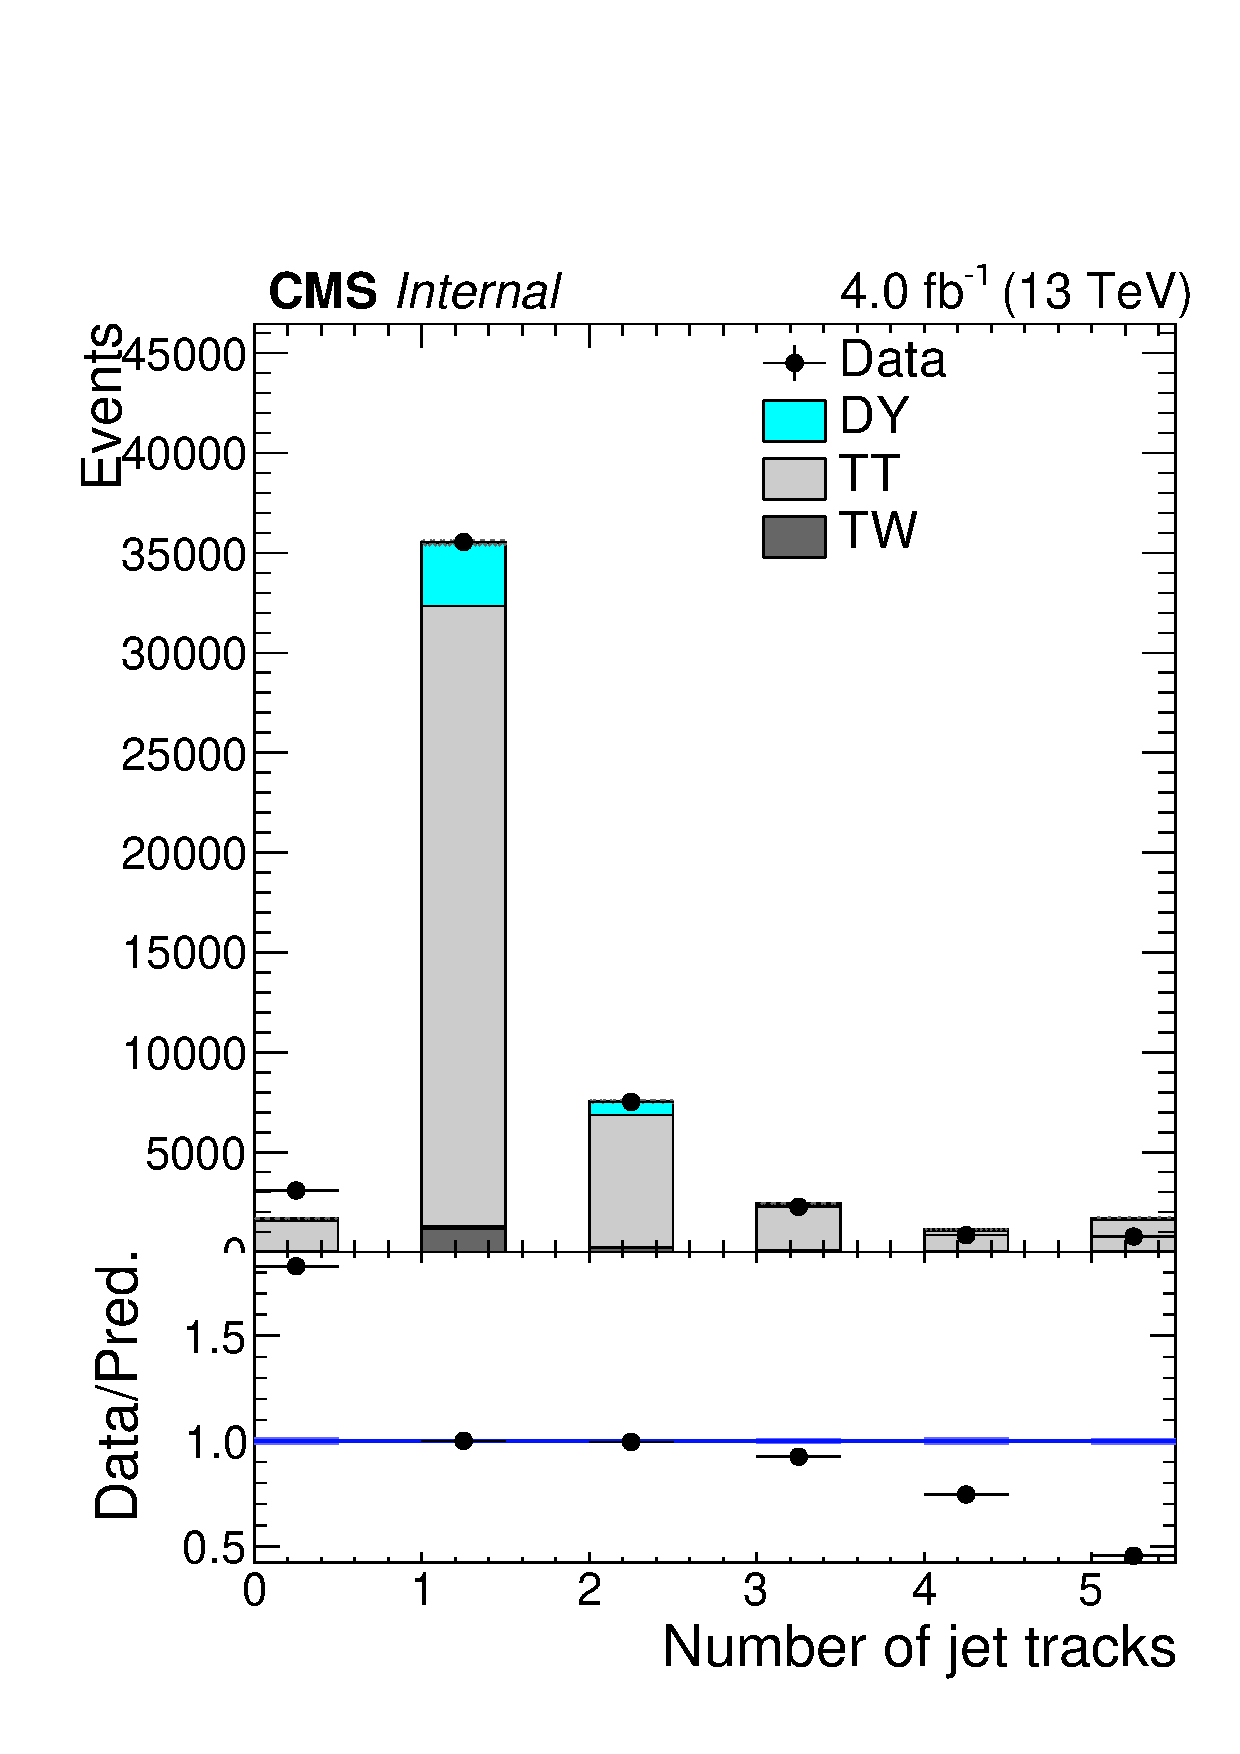
\includegraphics[width=0.32\textwidth]{plots_controlregions/leptons/ttbar/lep_jetNDauChargedMVASel.pdf}\\
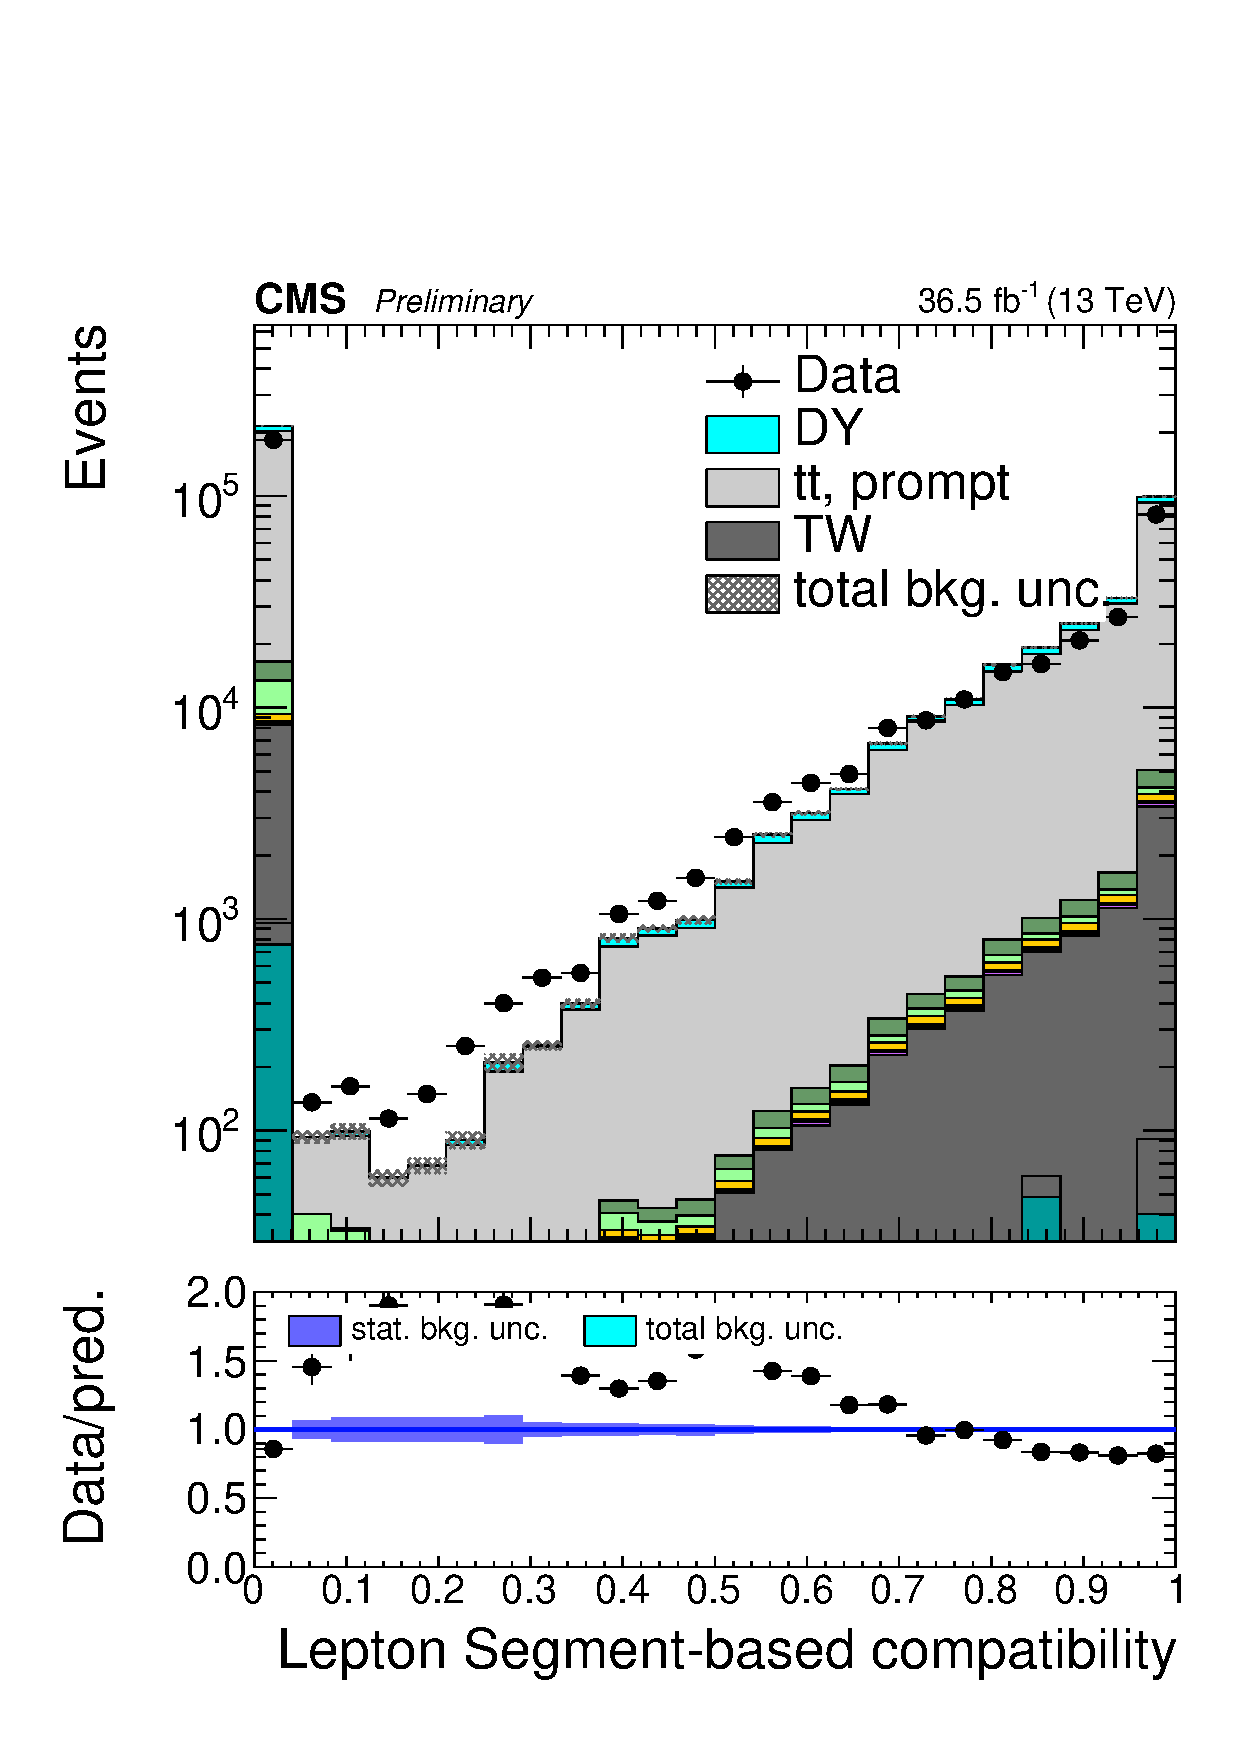
\includegraphics[width=0.32\textwidth]{plots_controlregions/leptons/ttbar/lep_SegmentCompatibility_log.pdf}
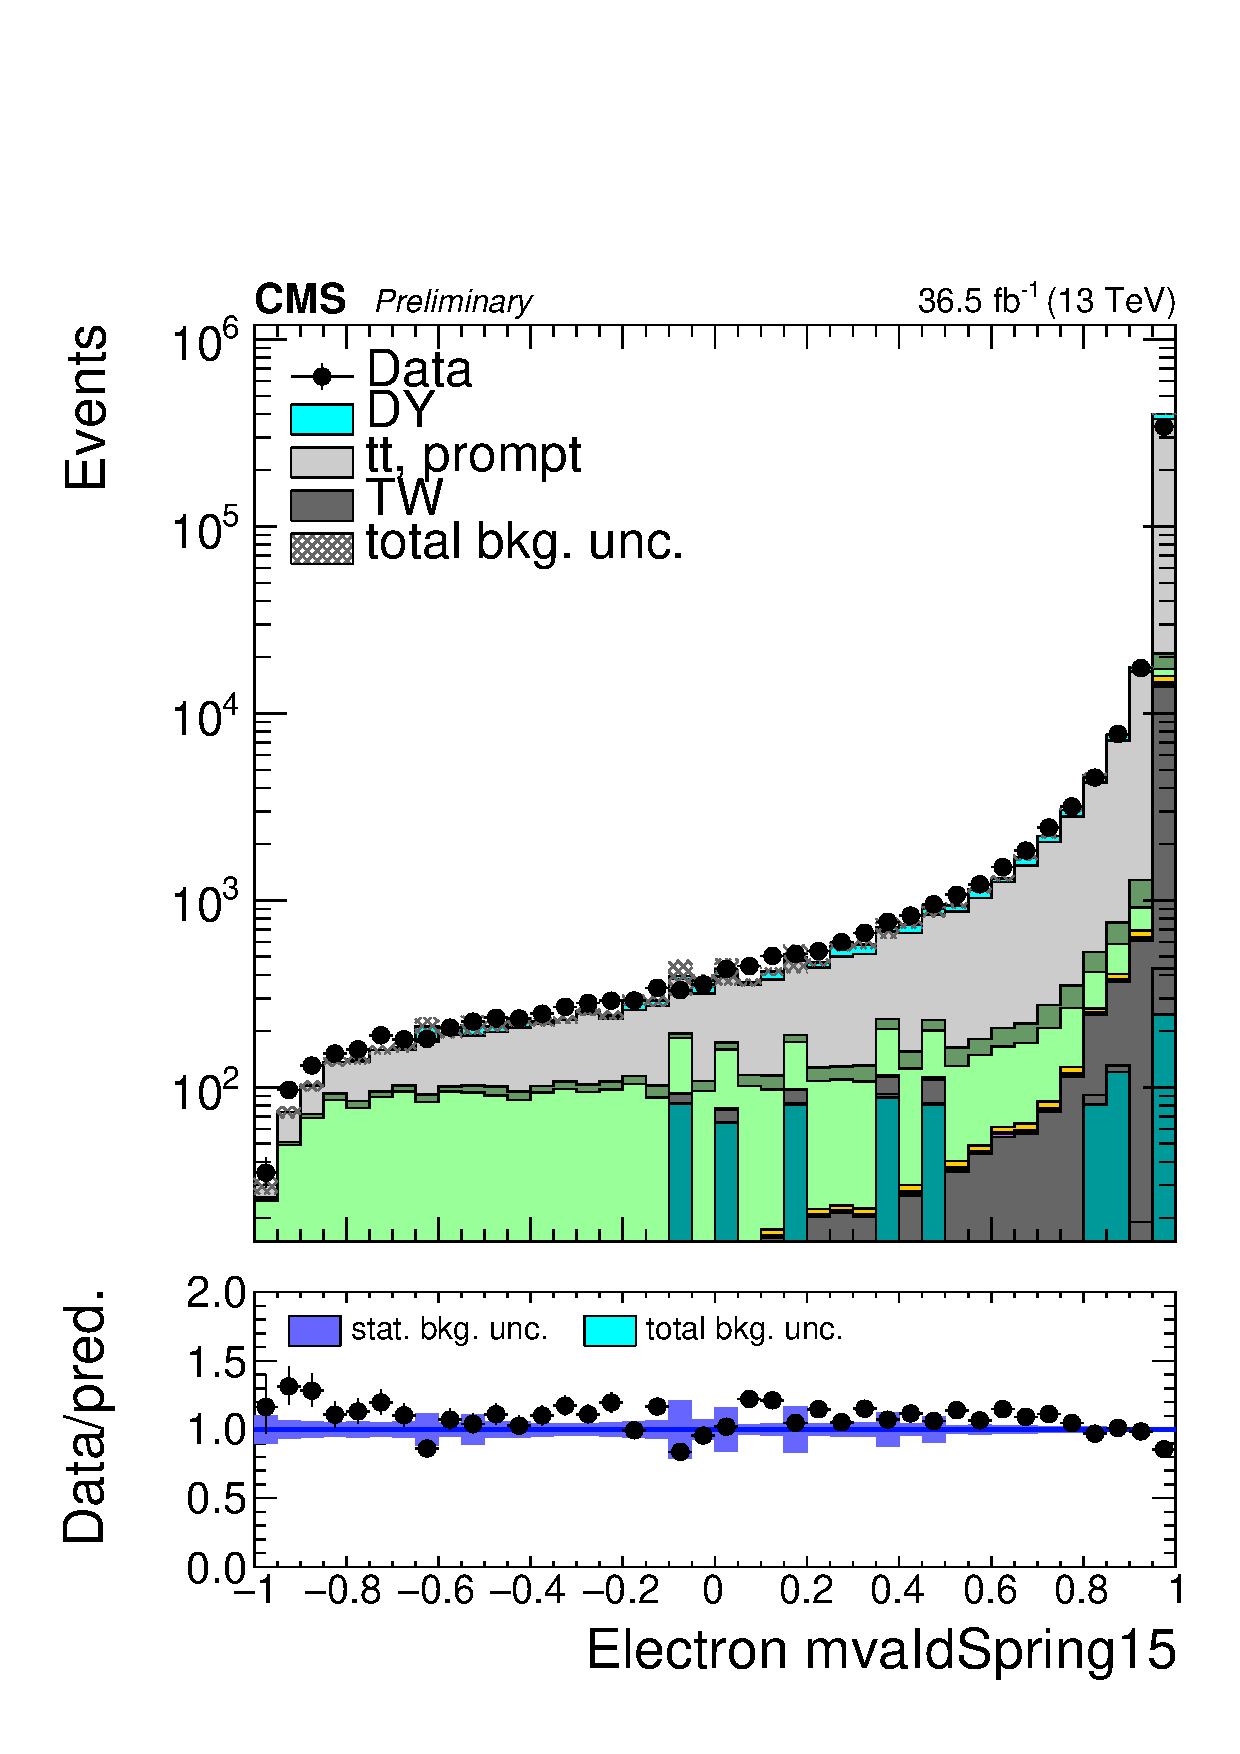
\includegraphics[width=0.32\textwidth]{plots_controlregions/leptons/ttbar/el_mvaIdSpring15_log.pdf}
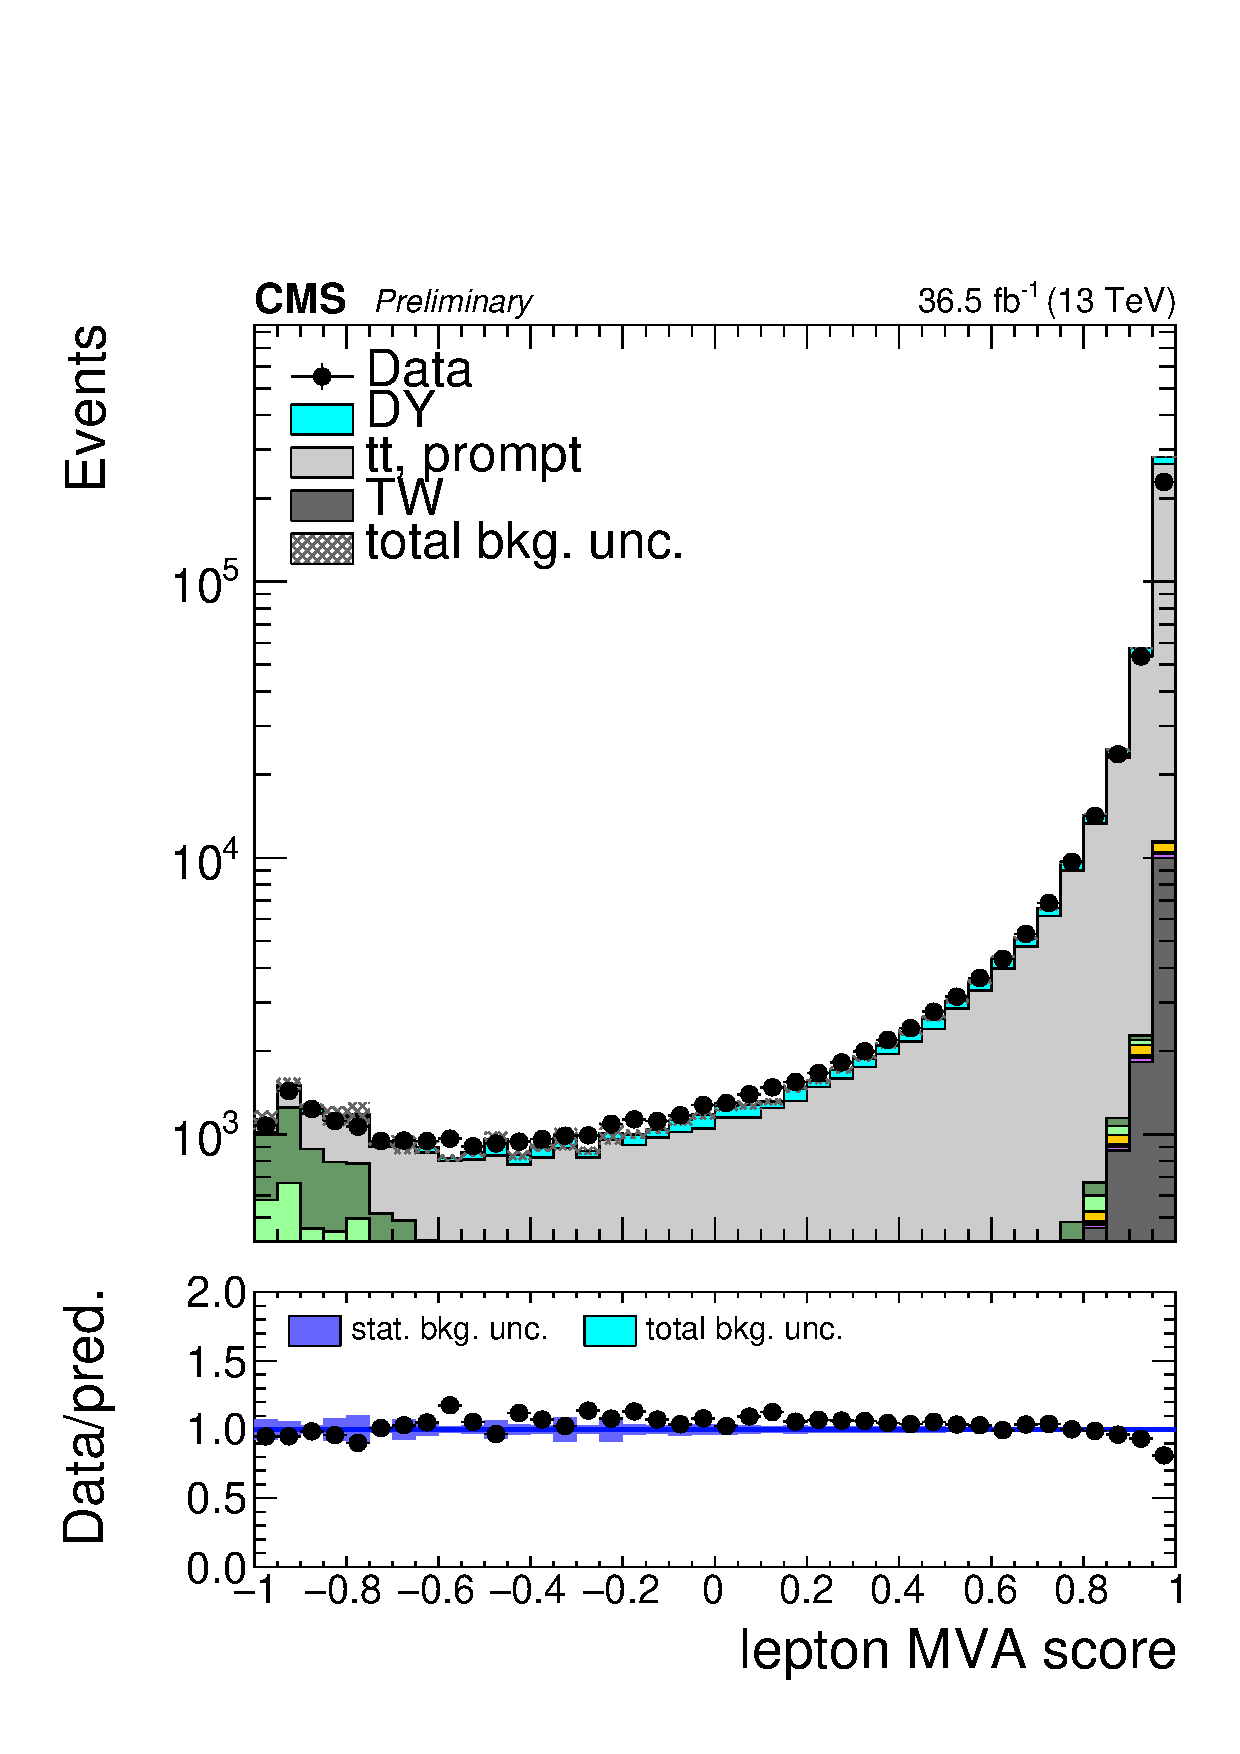
\includegraphics[width=0.32\textwidth]{plots_controlregions/leptons/ttbar/lep_mvaTTH_log.pdf}
        \caption{Summary of the input variables (continued) to the lepton MVA and output discriminator in a ttbar enriched sample, in data and simulation. The uncertainty shown on the simulation is only statistical.}
        \label{fig:lep-distributions-4}
\end{figure}

\newpage
\subsubsection{Loose selection efficiency}\label{sec:looseeff}
The reconstruction and loose identification efficiency are computed
both for muons and electrons using the Tag and Probe technique
with $Z\rightarrow\ell^{+}\ell^{-}$ events, in data and in simulation
separately.
The efficiency scale factor is therefore defined as:
\begin{equation}
  \rho(\pt,\eta) = \frac{\varepsilon_{\rm{data}}(\pt,\eta)}{\varepsilon_{\rm{MC}}(\pt,\eta)},
\end{equation}
where $\varepsilon_{\rm{i}}(\pt,\eta)$ is the efficiency measured for a given lepton in the process i (data or simulation). The scale factor is used afterward to correct the weight of the simulated event.
The full simulation correction from the lepton side is thus given by the product of all scale factors :
\begin{equation}
\rho = \prod_{j \in \rm{leptons}} \rho(\pt(j),\eta_j)
\end{equation}
We apply scale factors for the loose electron selection efficiency that have been derived in the context of the SUSY lepton SF working group.
%In Fig.~\ref{fig:electronTnP} the scale
%factors for the loose electron selection (with the electron
%ID emulation cuts) are shown. 
%Figure~\ref{fig:muonTnP} shows the scale factors for the loose muon
%selection.
The efficiency of tight selection cuts has been measured with the same procedure, with respect to the loose selection.
Systematics on these scale-factors related to the method have been
evaluated and are of the order of 2\% for both lepton flavors, in all
the considered kinematic range.\\

%%% FILL WHEN AVAILABLE
%%% \begin{figure}[!htb]
%%% \centering
%%% \includegraphics[width=0.40\linewidth]{plots_lepEff/TnP_Ele_LooseMVAIDEmuLooseIP.pdf}
%%% \includegraphics[width=0.40\linewidth]{plots_lepEff/TnP_Ele_MiniIsoLoose.pdf} \\
%%% \includegraphics[width=0.40\linewidth]{plots_lepEff/TnP_Ele_ConvMissHits.pdf}
%%% \caption{From left to right: electron data to simulation scale factors for the
%%% Loose WP of the Electron MVA ID together with the Loose IP cuts and
%%% HLT ID Emulation requirements, for the Loose \miniIso, for the Tight
%%% cuts on the conversion veto and the missing inner hits}
%%% \label{fig:electronTnP}
%%% \end{figure}


%\begin{figure}[!hb]
%\centering
%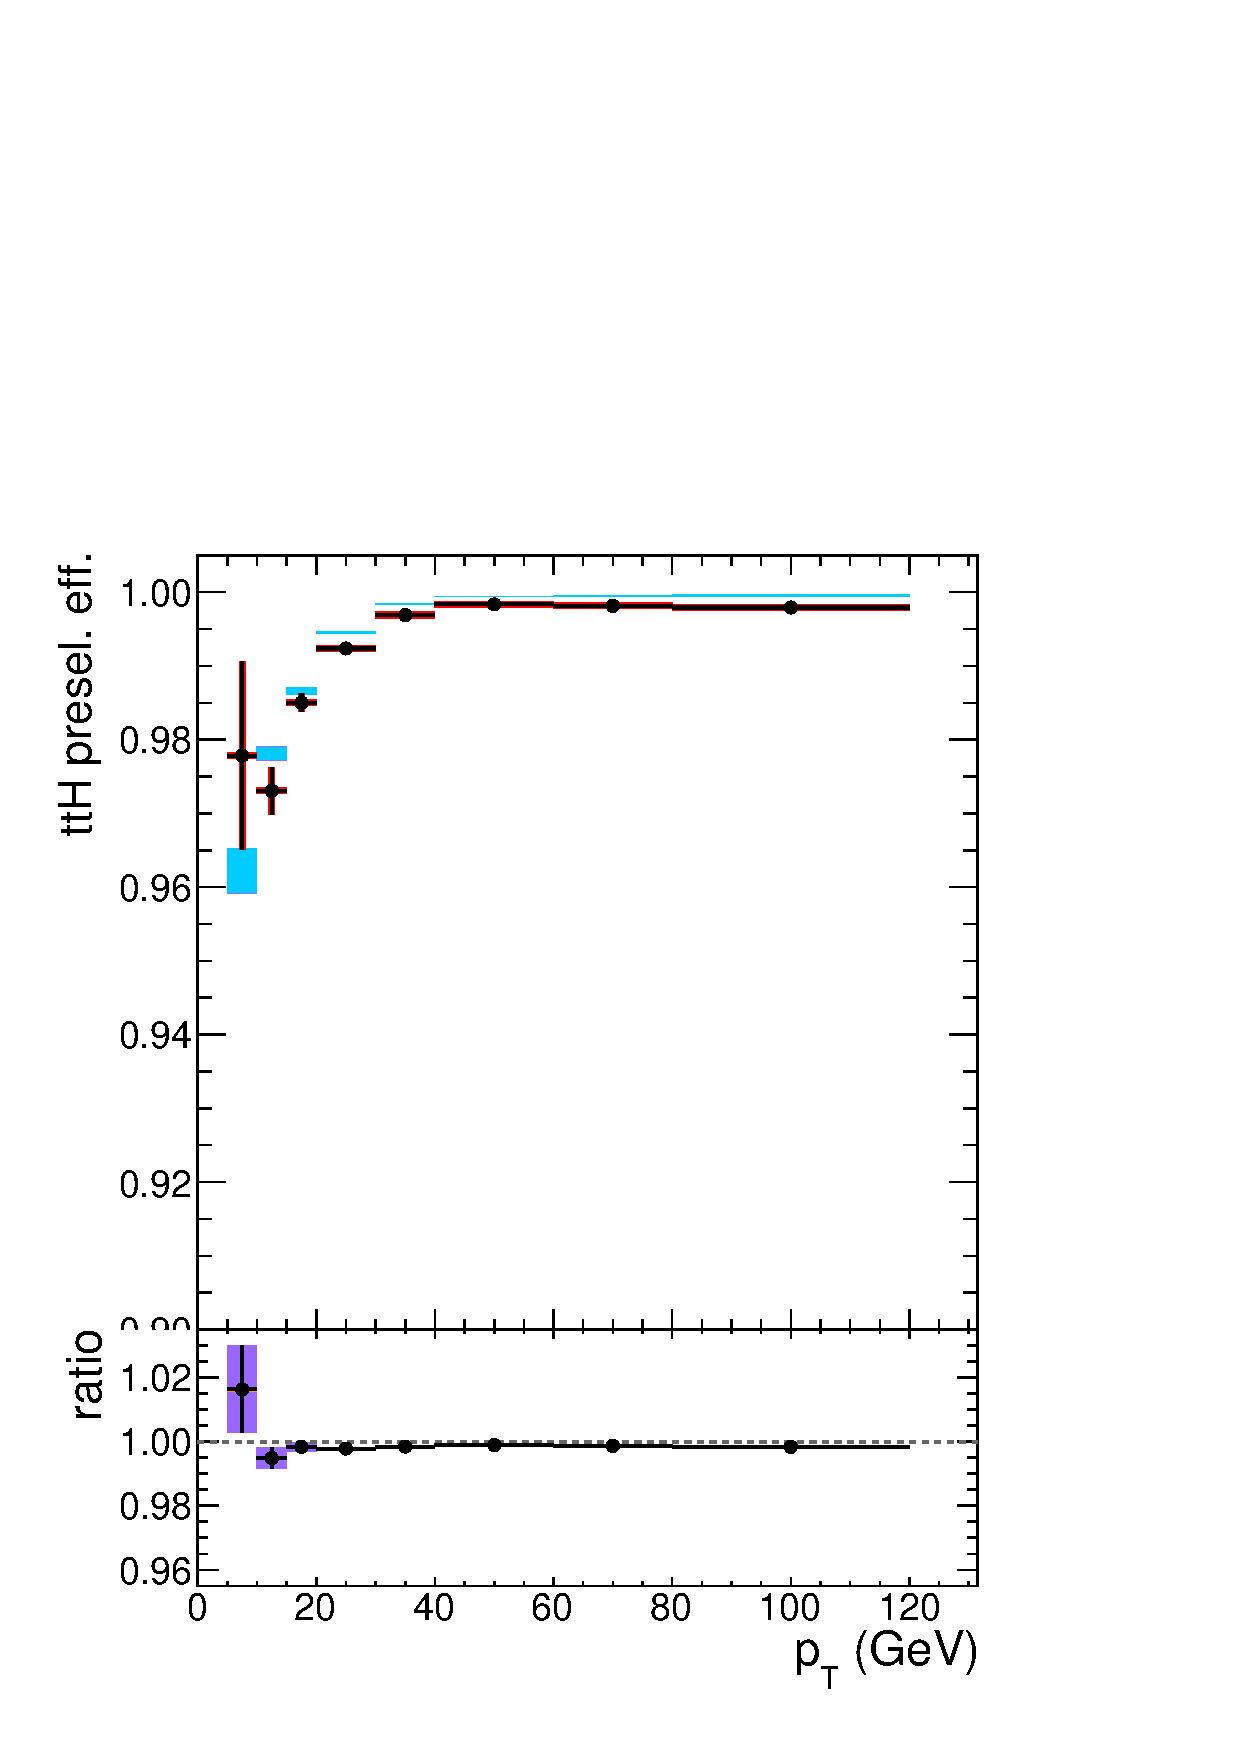
\includegraphics[width=0.30\linewidth]{plots_lepEff/GioEff/mu_ttHPresel_barrel.pdf}
%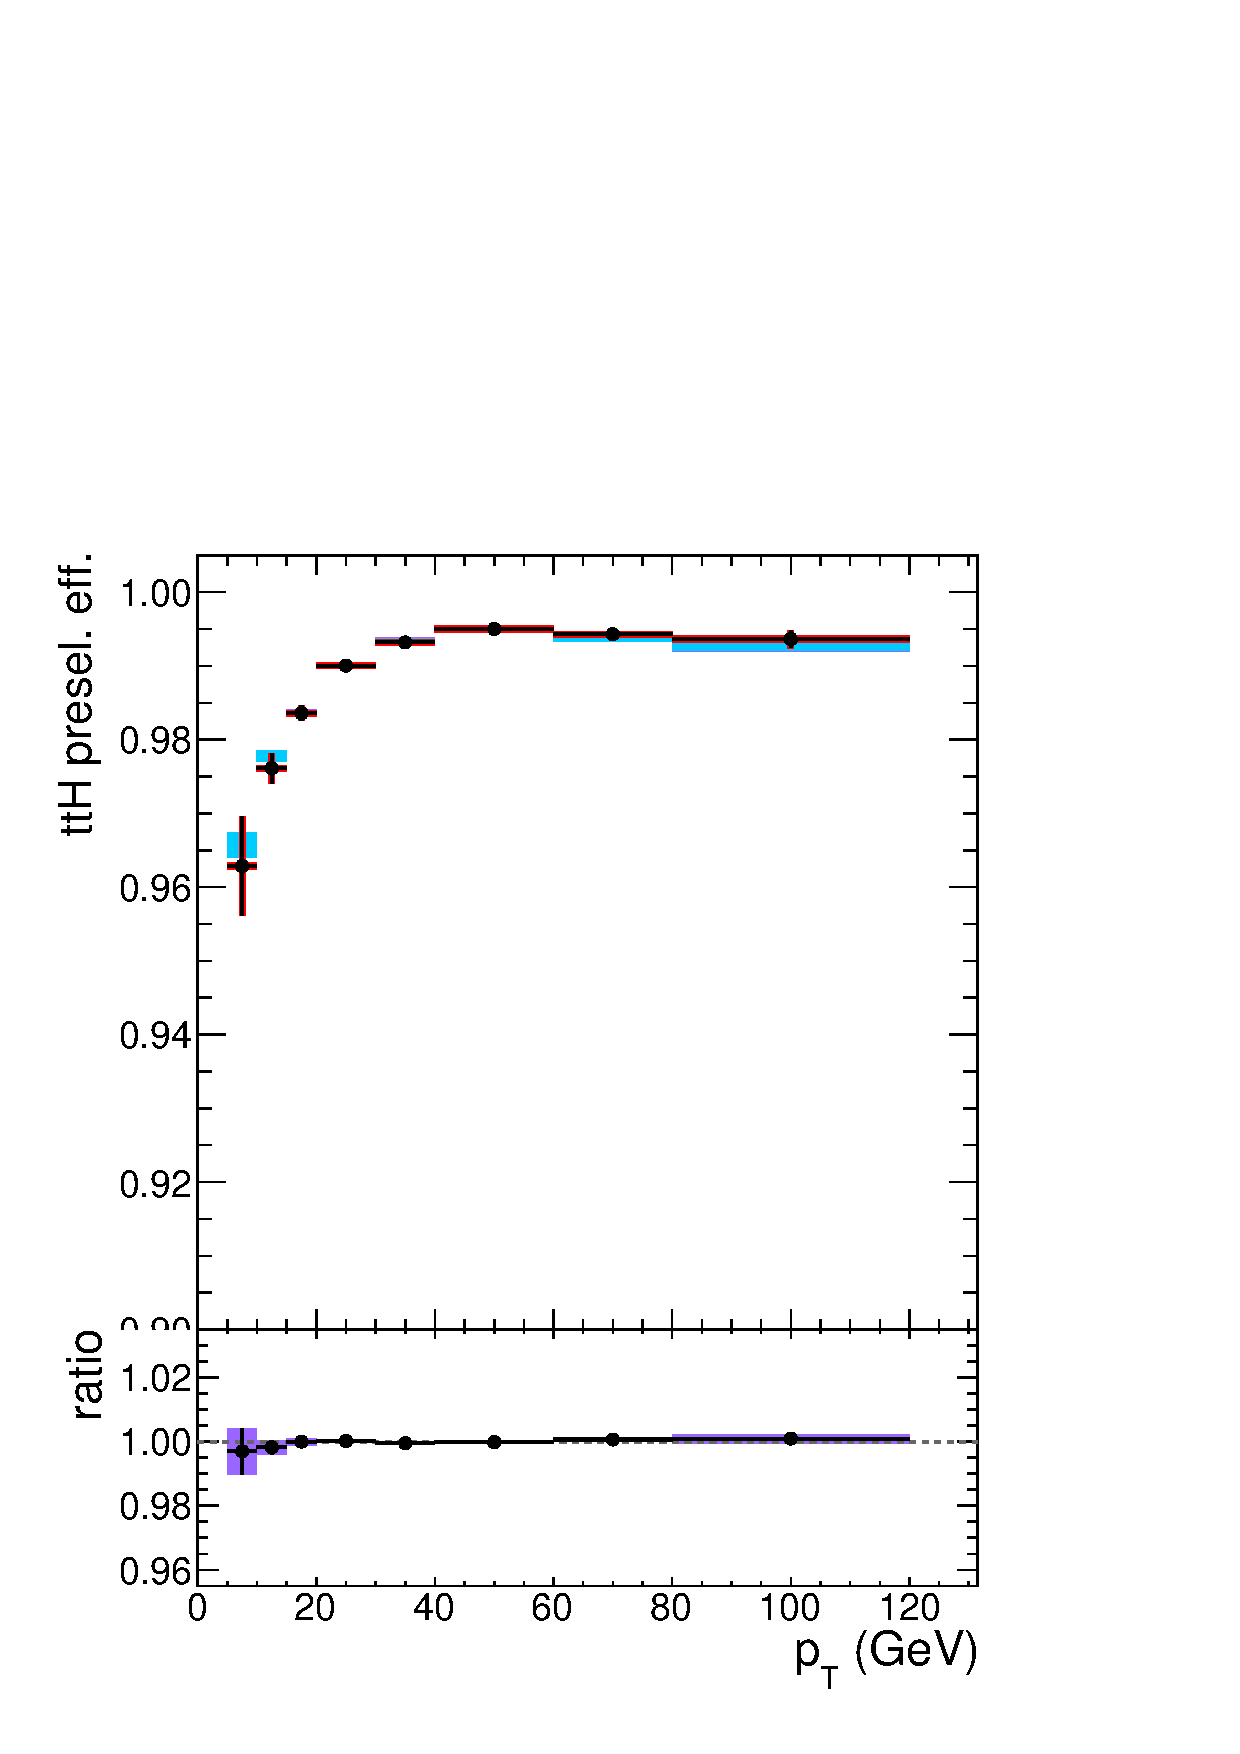
\includegraphics[width=0.30\linewidth]{plots_lepEff/GioEff/mu_ttHPresel_endcap.pdf}\\
%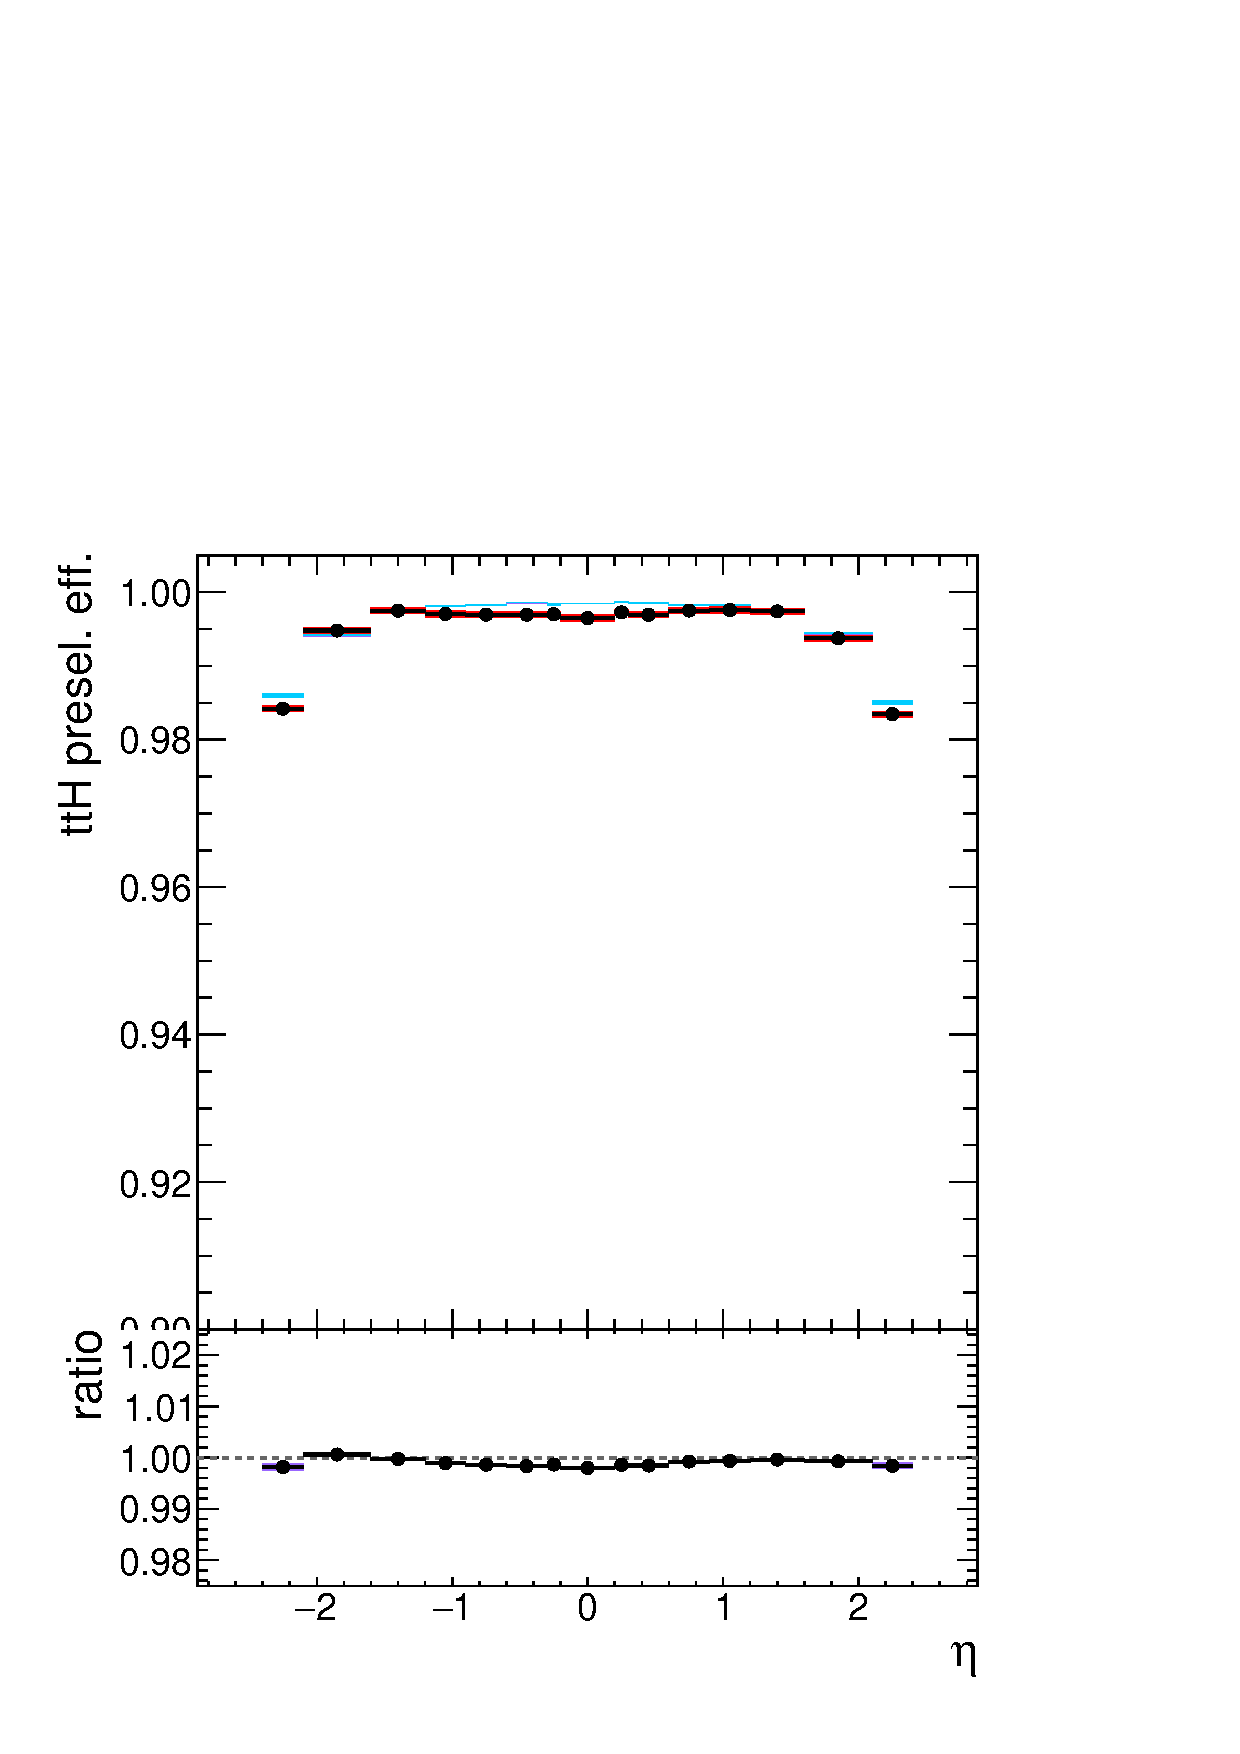
\includegraphics[width=0.30\linewidth]{plots_lepEff/GioEff/mu_ttHPresel_pt20.pdf}
%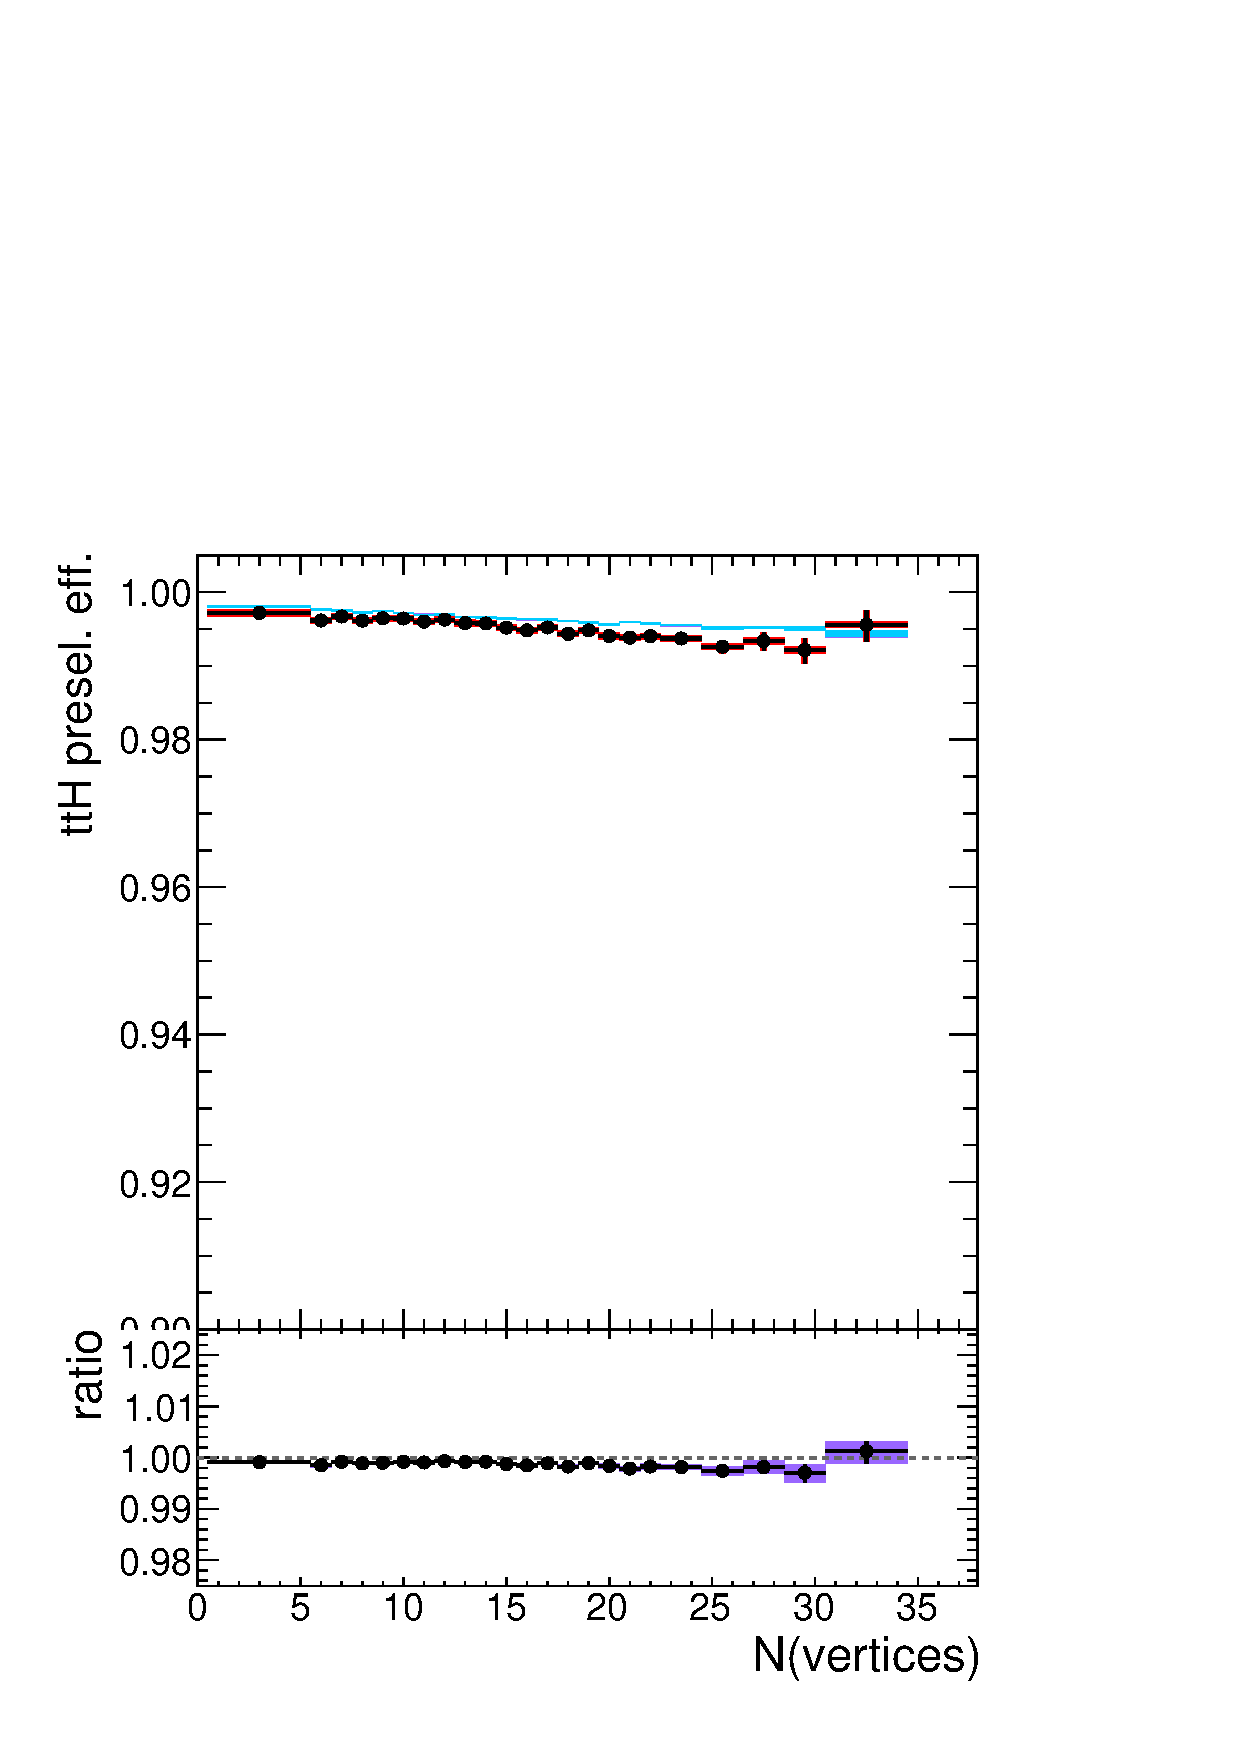
\includegraphics[width=0.30\linewidth]{plots_lepEff/GioEff/mu_ttHPresel_pt20_vtx.pdf}
%\caption{From left to right: muon data and simulation efficiency for
%  the preselection (SIP $<$ 8, miniRelIso $<$ 0.4) requirement in the barrel and endcap regions,
%  and muon data and simulation efficiency for the loose impact parameters cuts.}
%\label{fig:muonTnP}
%\end{figure}

\subsubsection{Tight vs Loose selection efficiency}
The efficiencies of applying the tight selection as defined in Tables~\ref{tab:muonIDs} and~\ref{tab:eleIDs}, on the loose leptons are determined using a tag and probe method on a sample of DY-enriched events.
% The denominator definitions for these efficiencies includes the $\text{SIP}_{3D} < 8$ as it is already included in the loose lepton efficiencies described in Section~\ref{sec:looseeff}.
Numerator cuts for the same-sign dilepton efficiencies include the tight-charge requirement.

Number of passed and failed probes are determined from a fit to the invariant mass of the dilepton system.
The resulting efficiencies are shown in Figures~\ref{fig:electronMVAEff_2lss}, \ref{fig:muonMVAEff_2lss}, \ref{fig:electronMVAEff_3l}, and~\ref{fig:muonMVAEff_3l}.

\begin{figure}[!hb]
\centering
  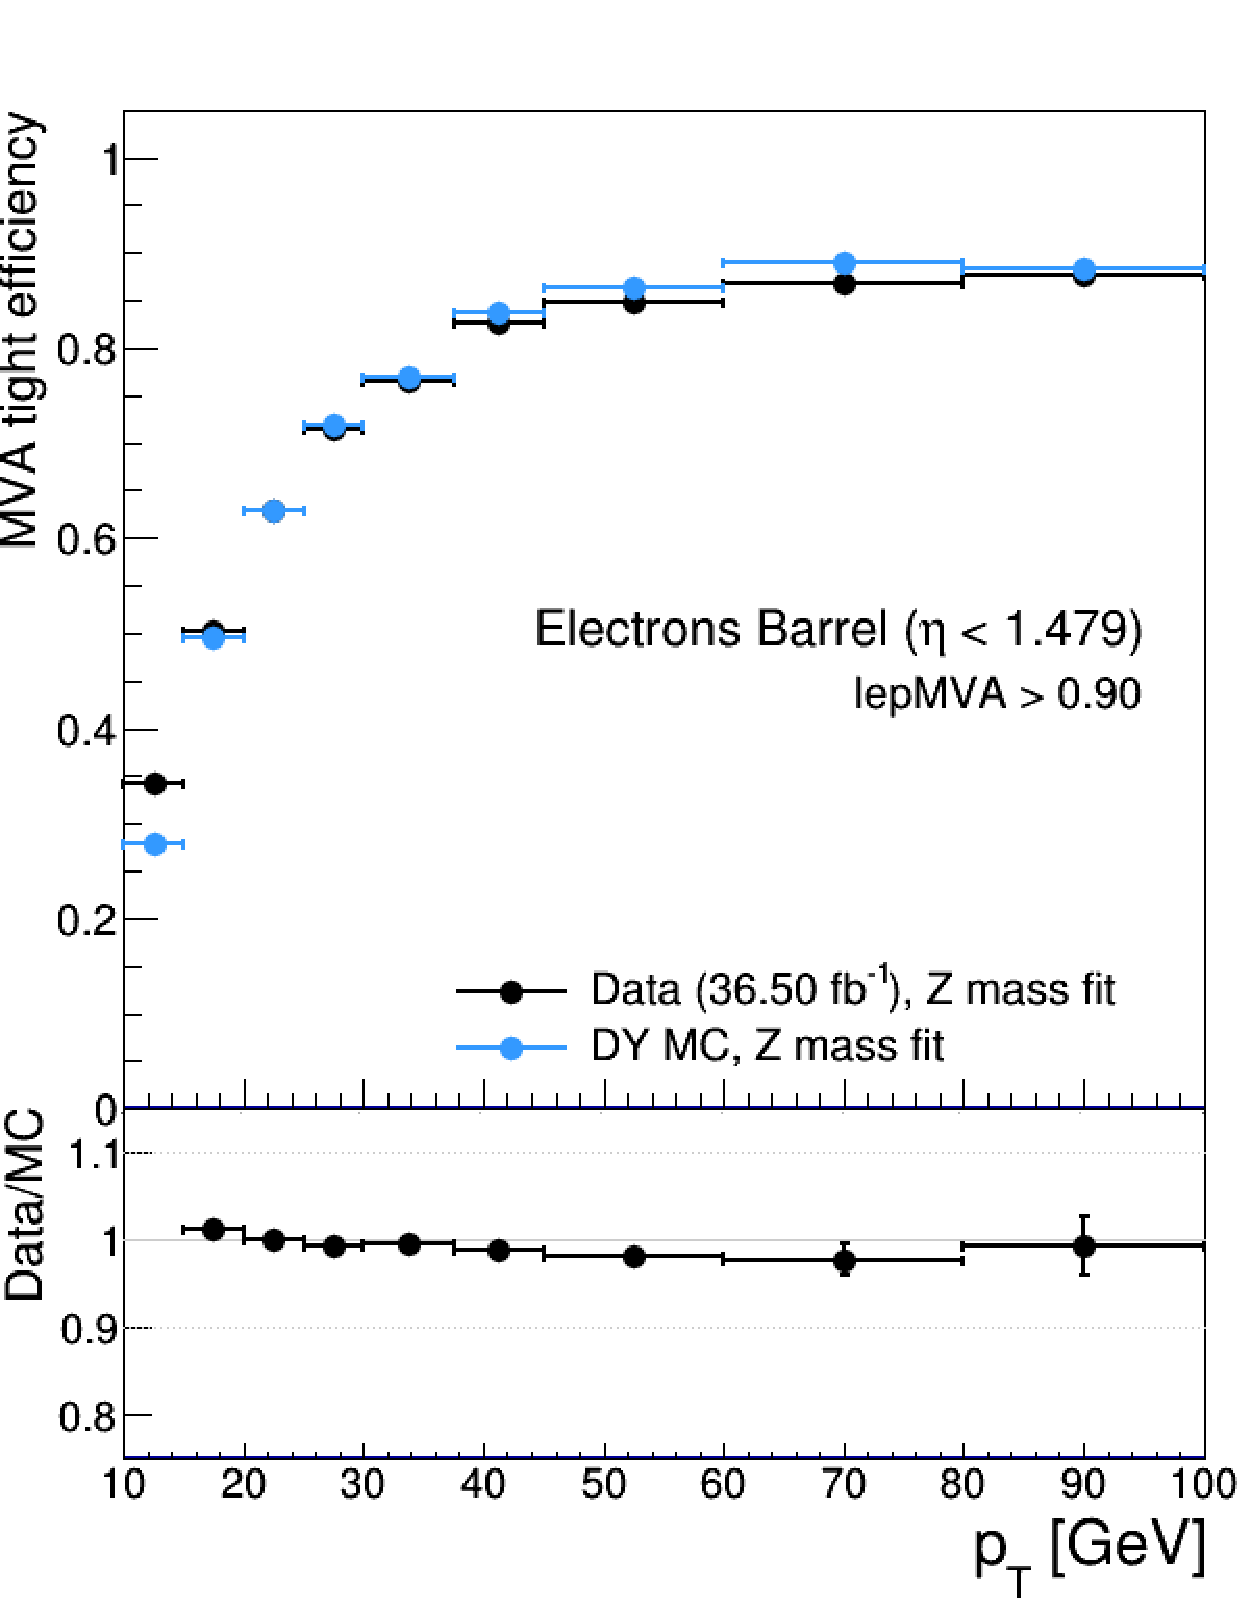
\includegraphics[width=0.31\linewidth]{plots_leptons/lepmva_efficiency/tnp_eff_eb_2lss_pt.pdf}  
  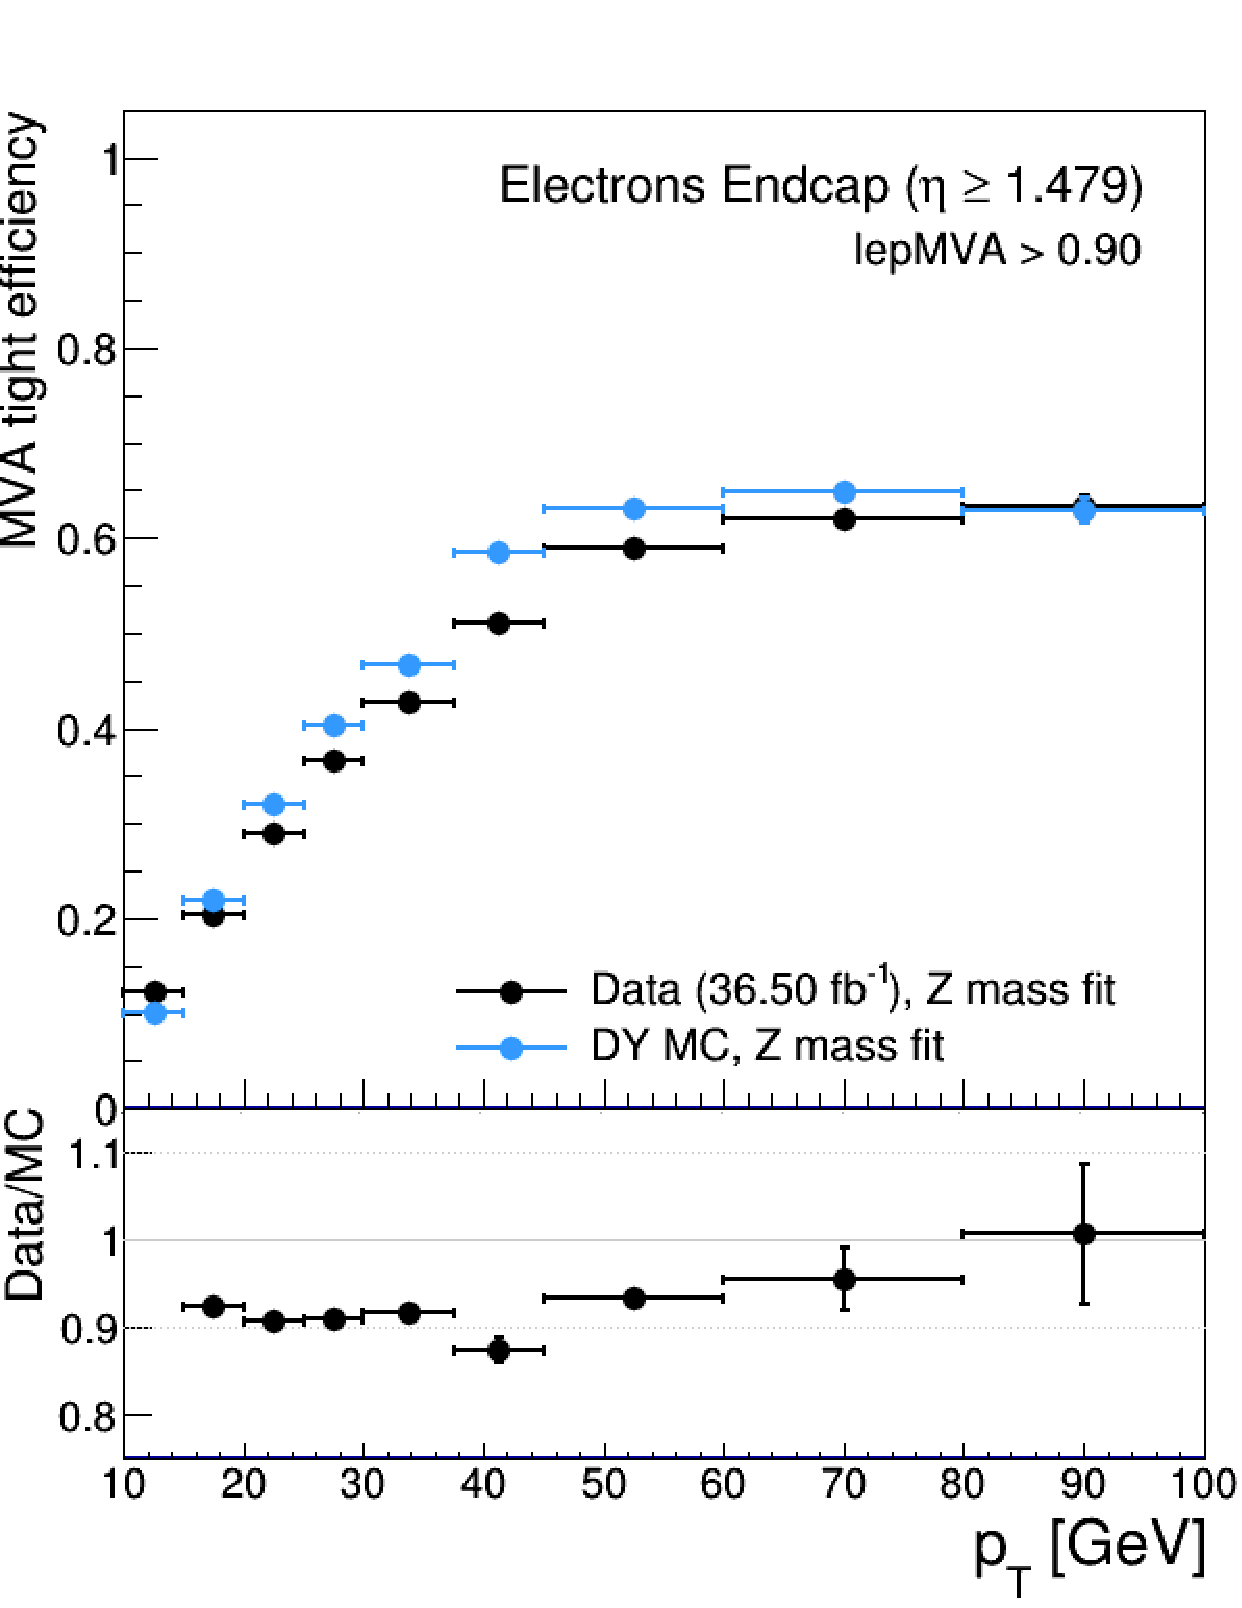
\includegraphics[width=0.31\linewidth]{plots_leptons/lepmva_efficiency/tnp_eff_ee_2lss_pt.pdf}
  %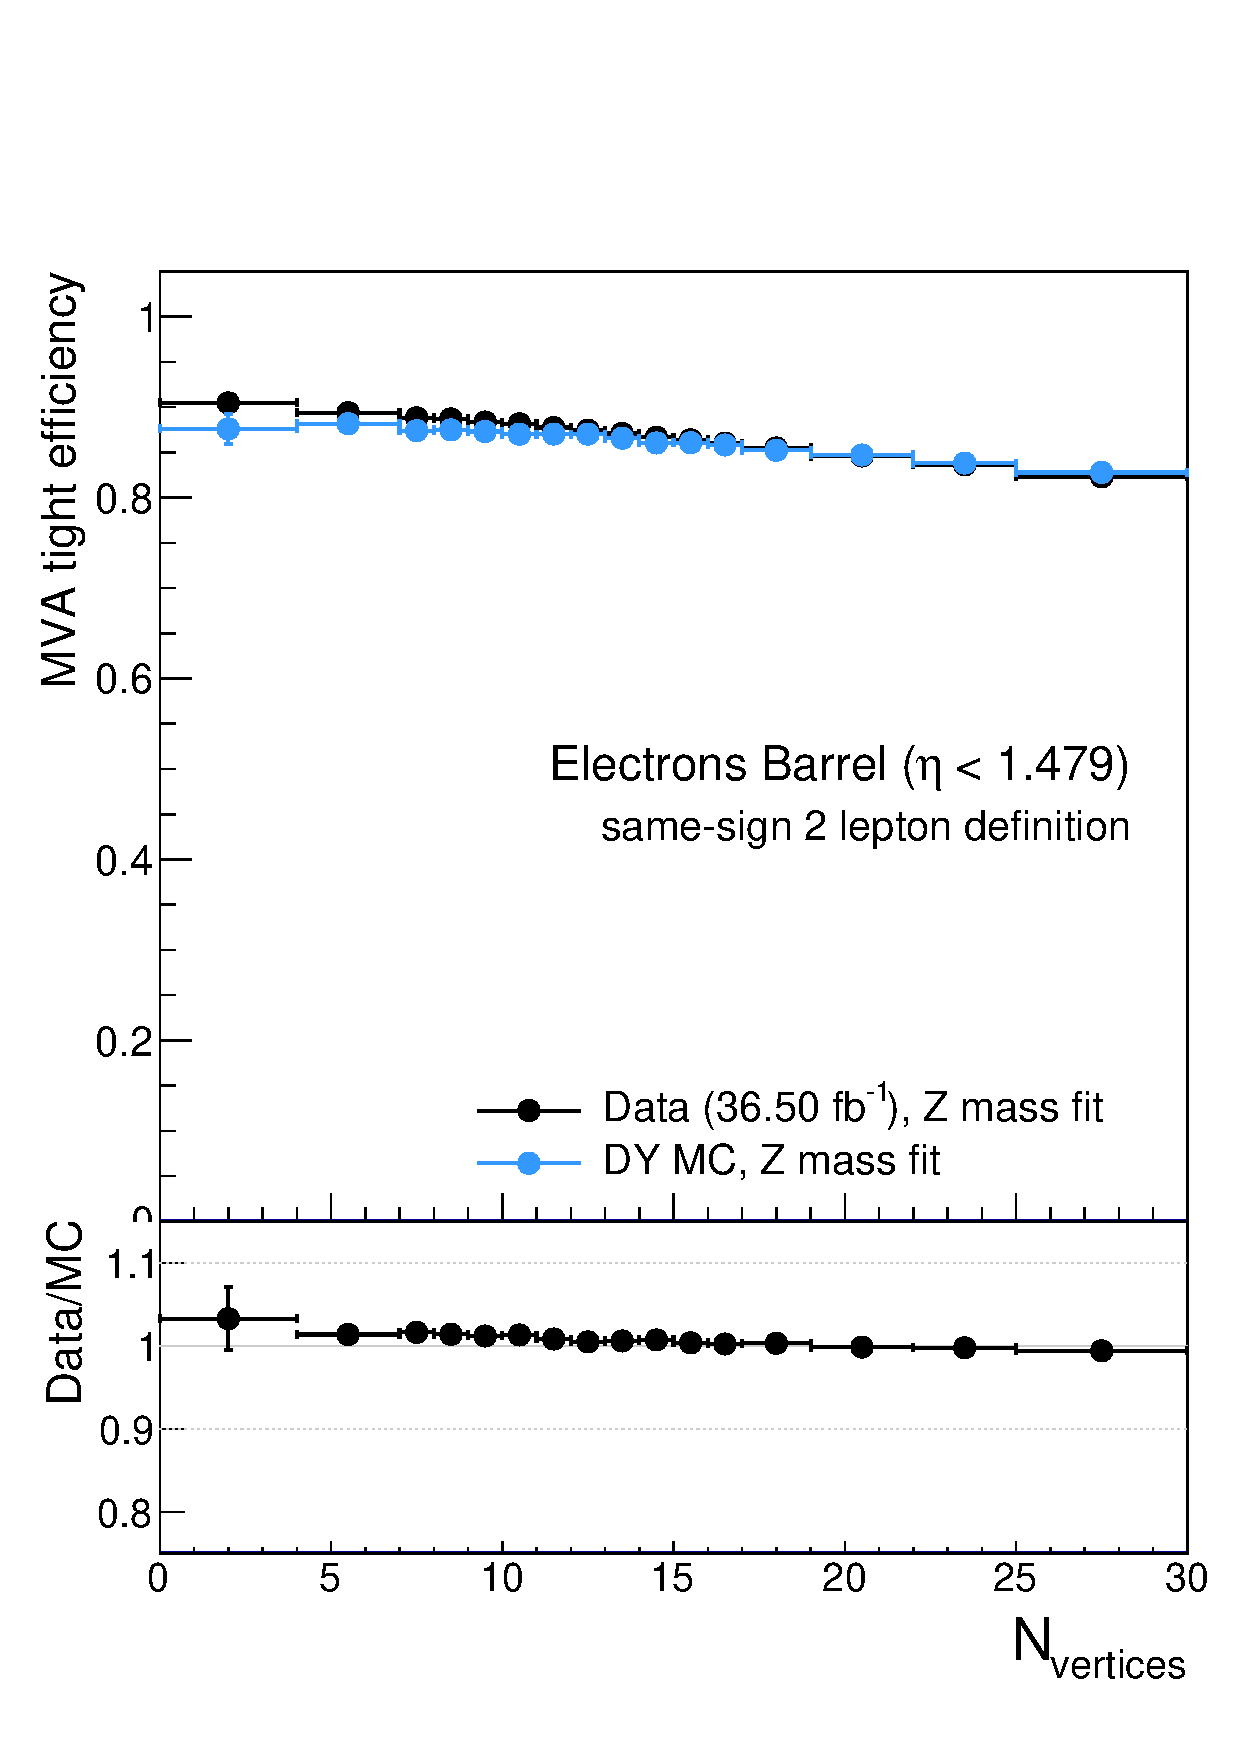
\includegraphics[width=0.31\linewidth]{plots_leptons/lepmva_efficiency/tnp_eff_eb_2lss_nVert.pdf}
\caption{Tight vs loose selection efficiencies for electrons, for the same-sign dilepton lepton definition (\ie\ including the tight-charge requirement).}
\label{fig:electronMVAEff_2lss}
\end{figure}

\begin{figure}[!ht]
\centering
  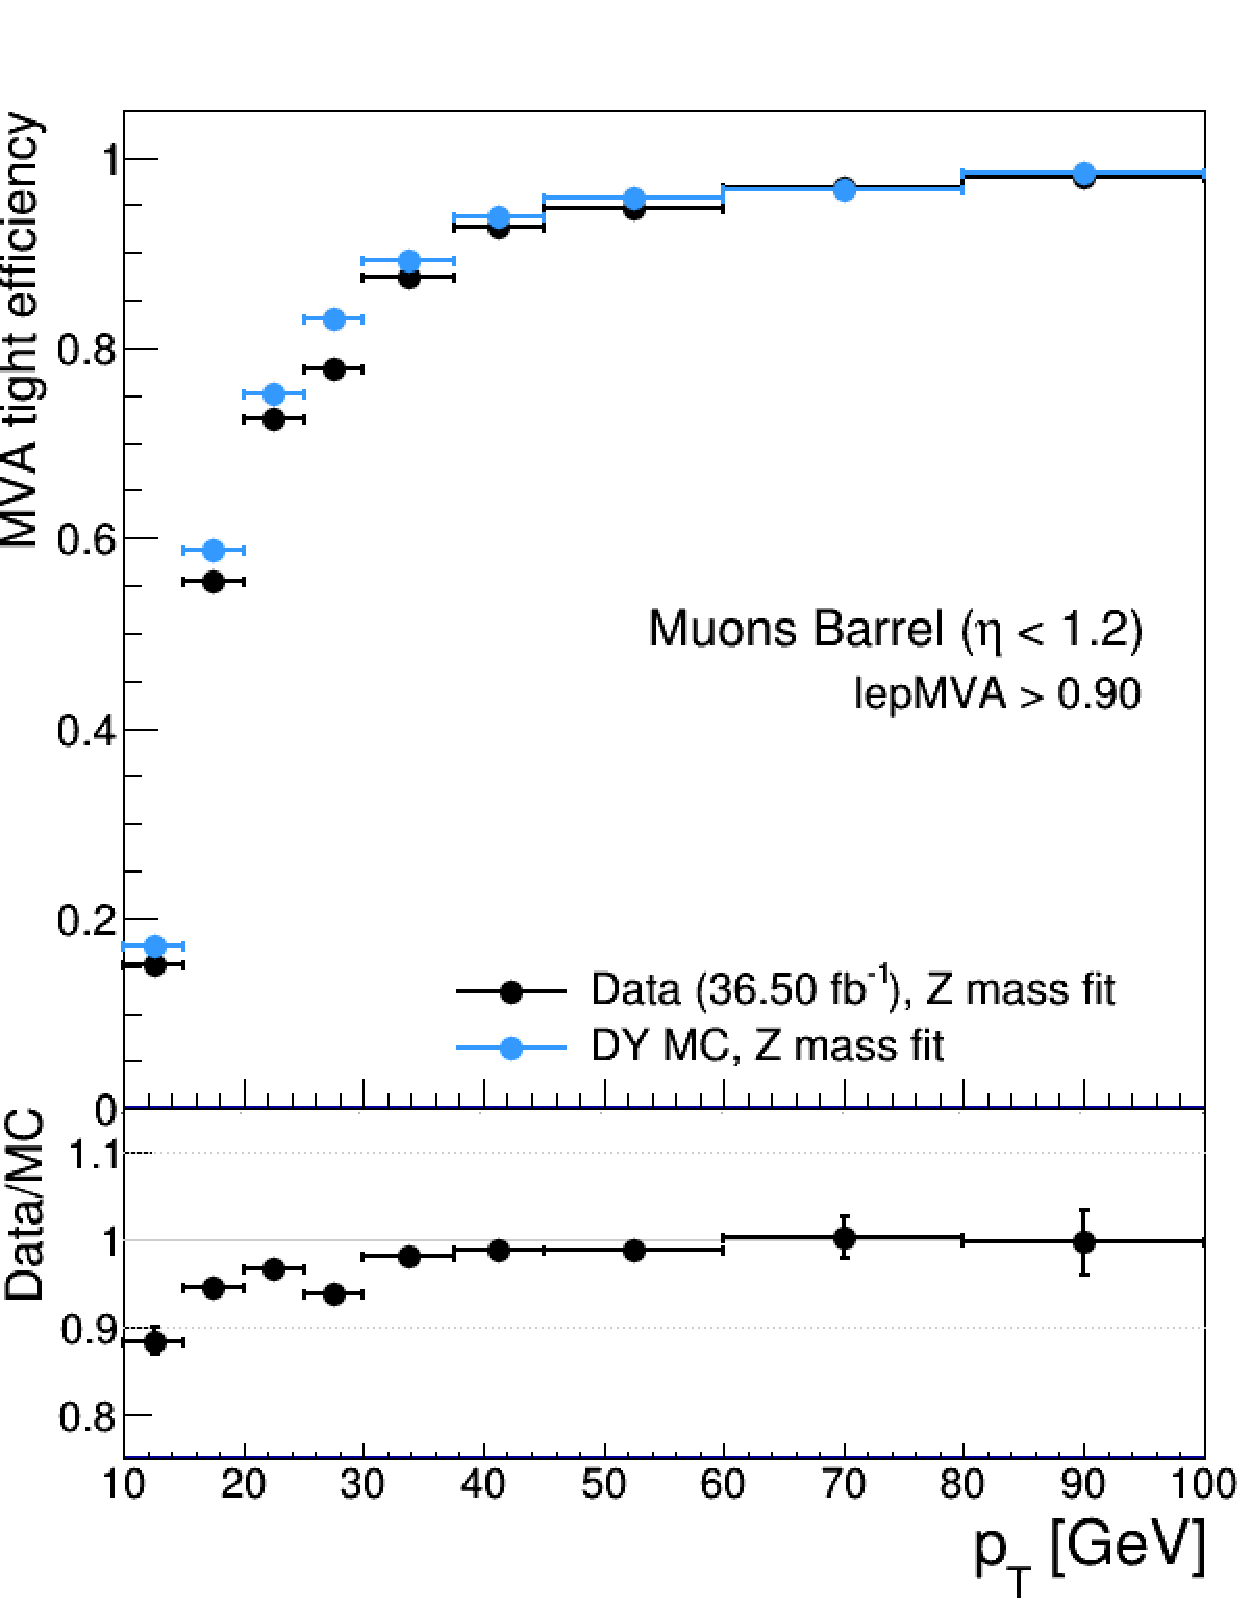
\includegraphics[width=0.31\linewidth]{plots_leptons/lepmva_efficiency/tnp_eff_mb_2lss_pt.pdf}
  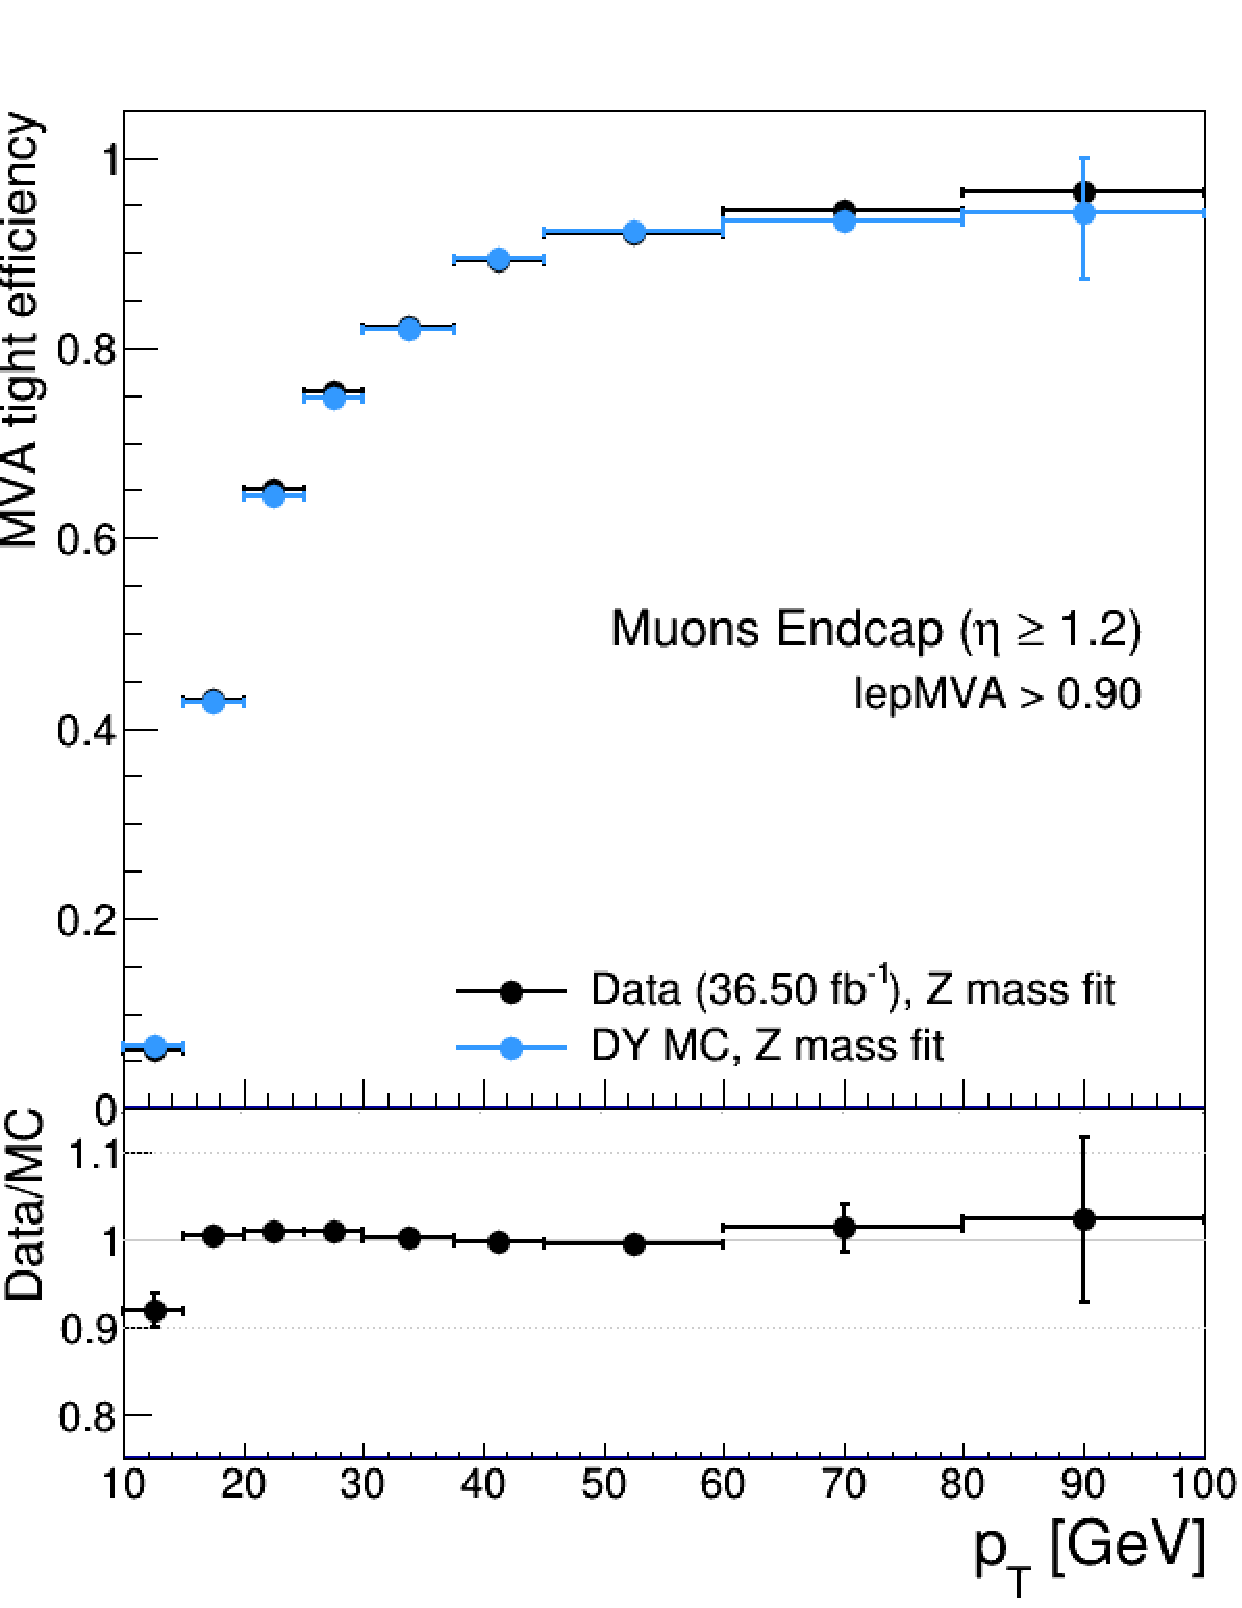
\includegraphics[width=0.31\linewidth]{plots_leptons/lepmva_efficiency/tnp_eff_me_2lss_pt.pdf}
  %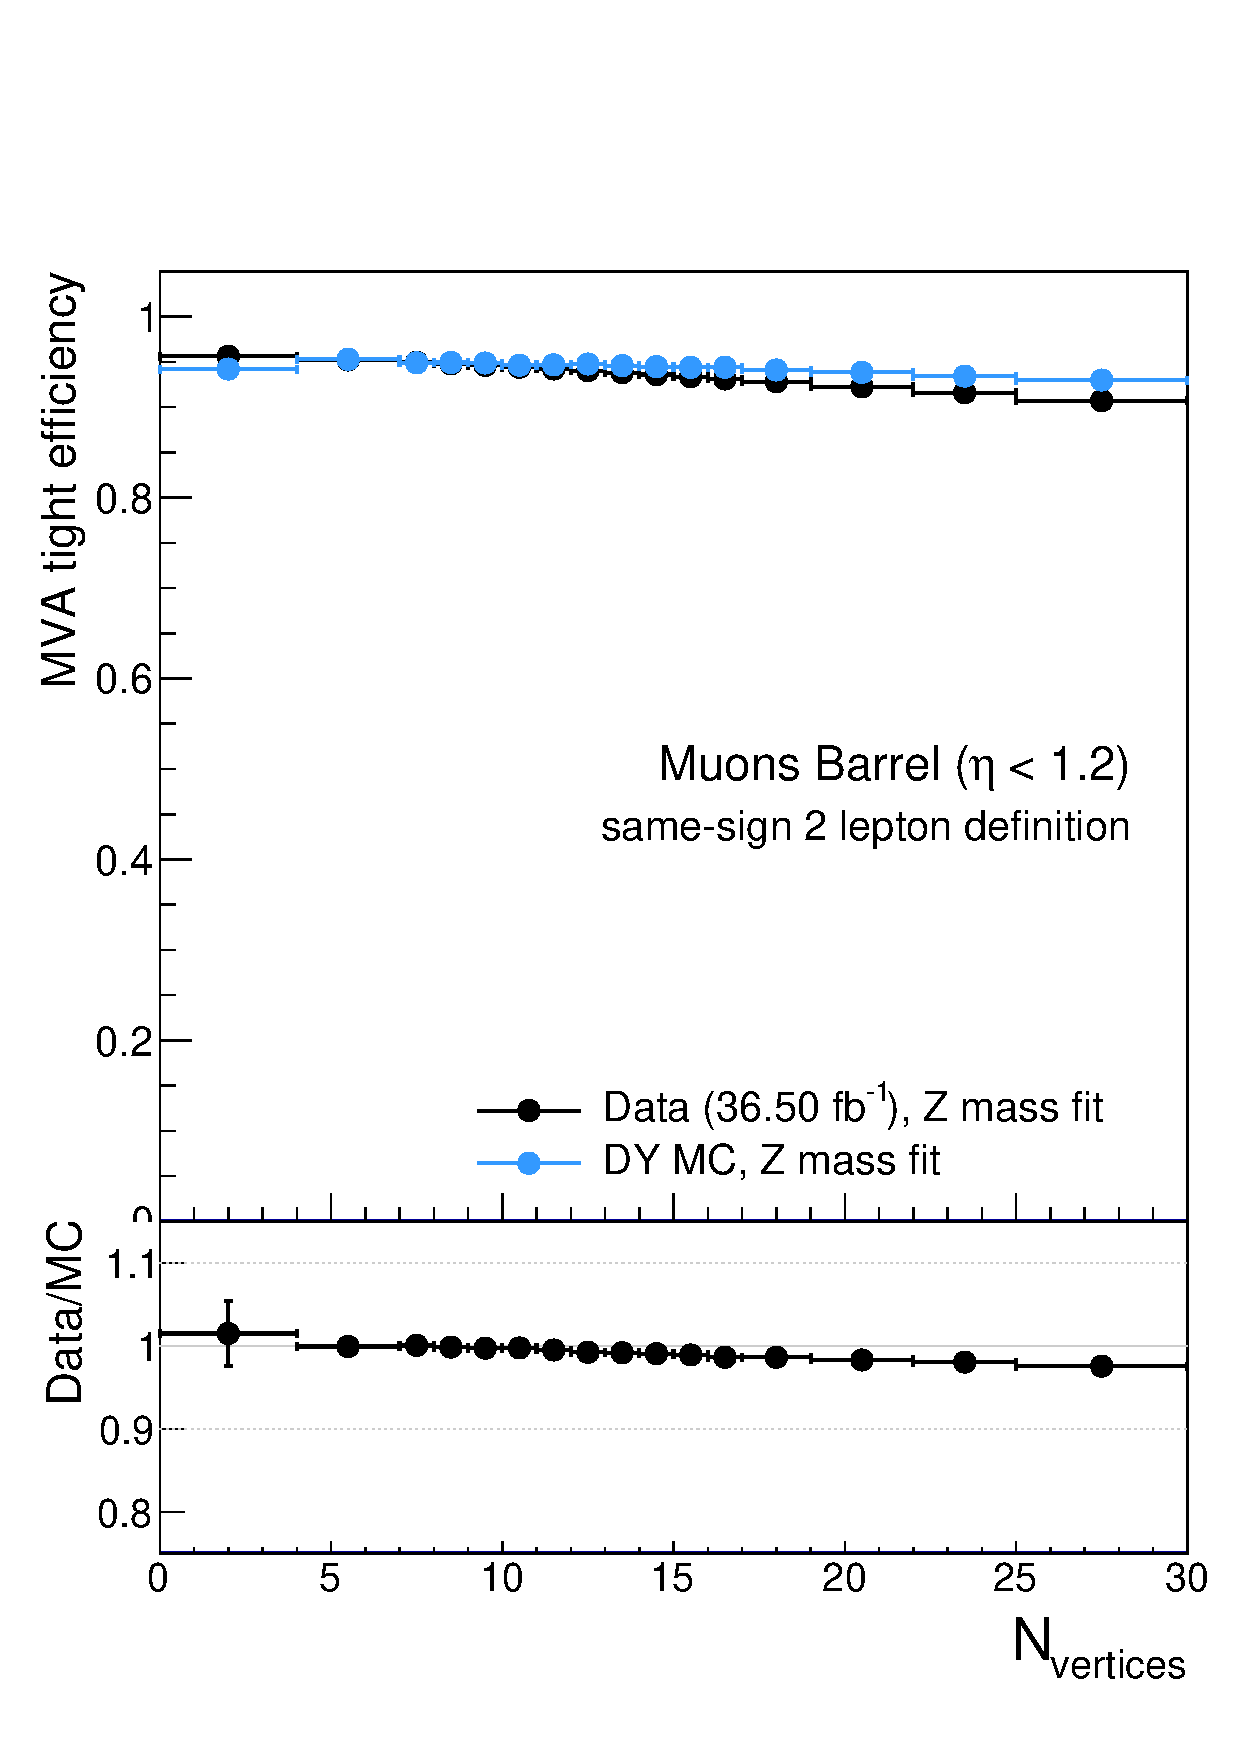
\includegraphics[width=0.31\linewidth]{plots_leptons/lepmva_efficiency/tnp_eff_mb_2lss_nVert.pdf}
\caption{Tight vs loose selection efficiencies for muons, for the same-sign dilepton lepton definition (\ie\ including the tight-charge requirement).}
\label{fig:muonMVAEff_2lss}
\end{figure}

\begin{figure}[!ht]
\centering
  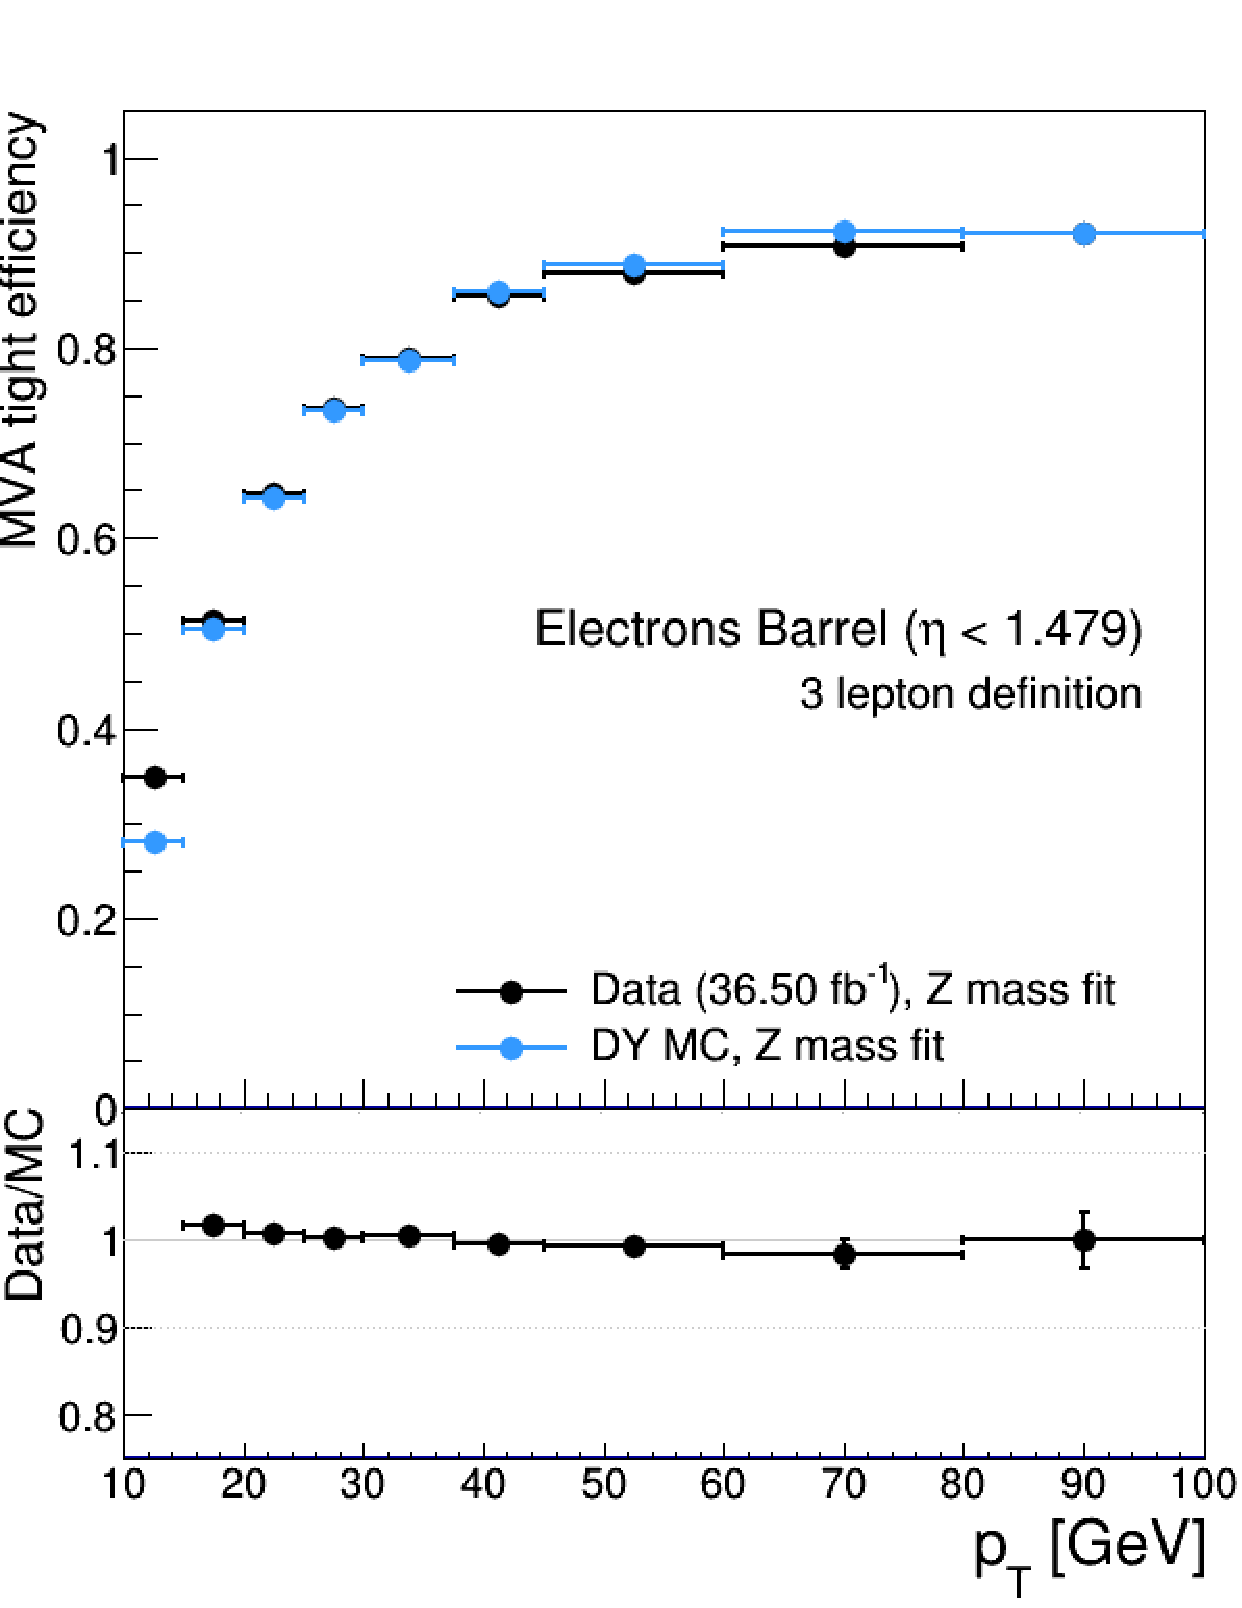
\includegraphics[width=0.31\linewidth]{plots_leptons/lepmva_efficiency/tnp_eff_eb_3l_pt.pdf}
  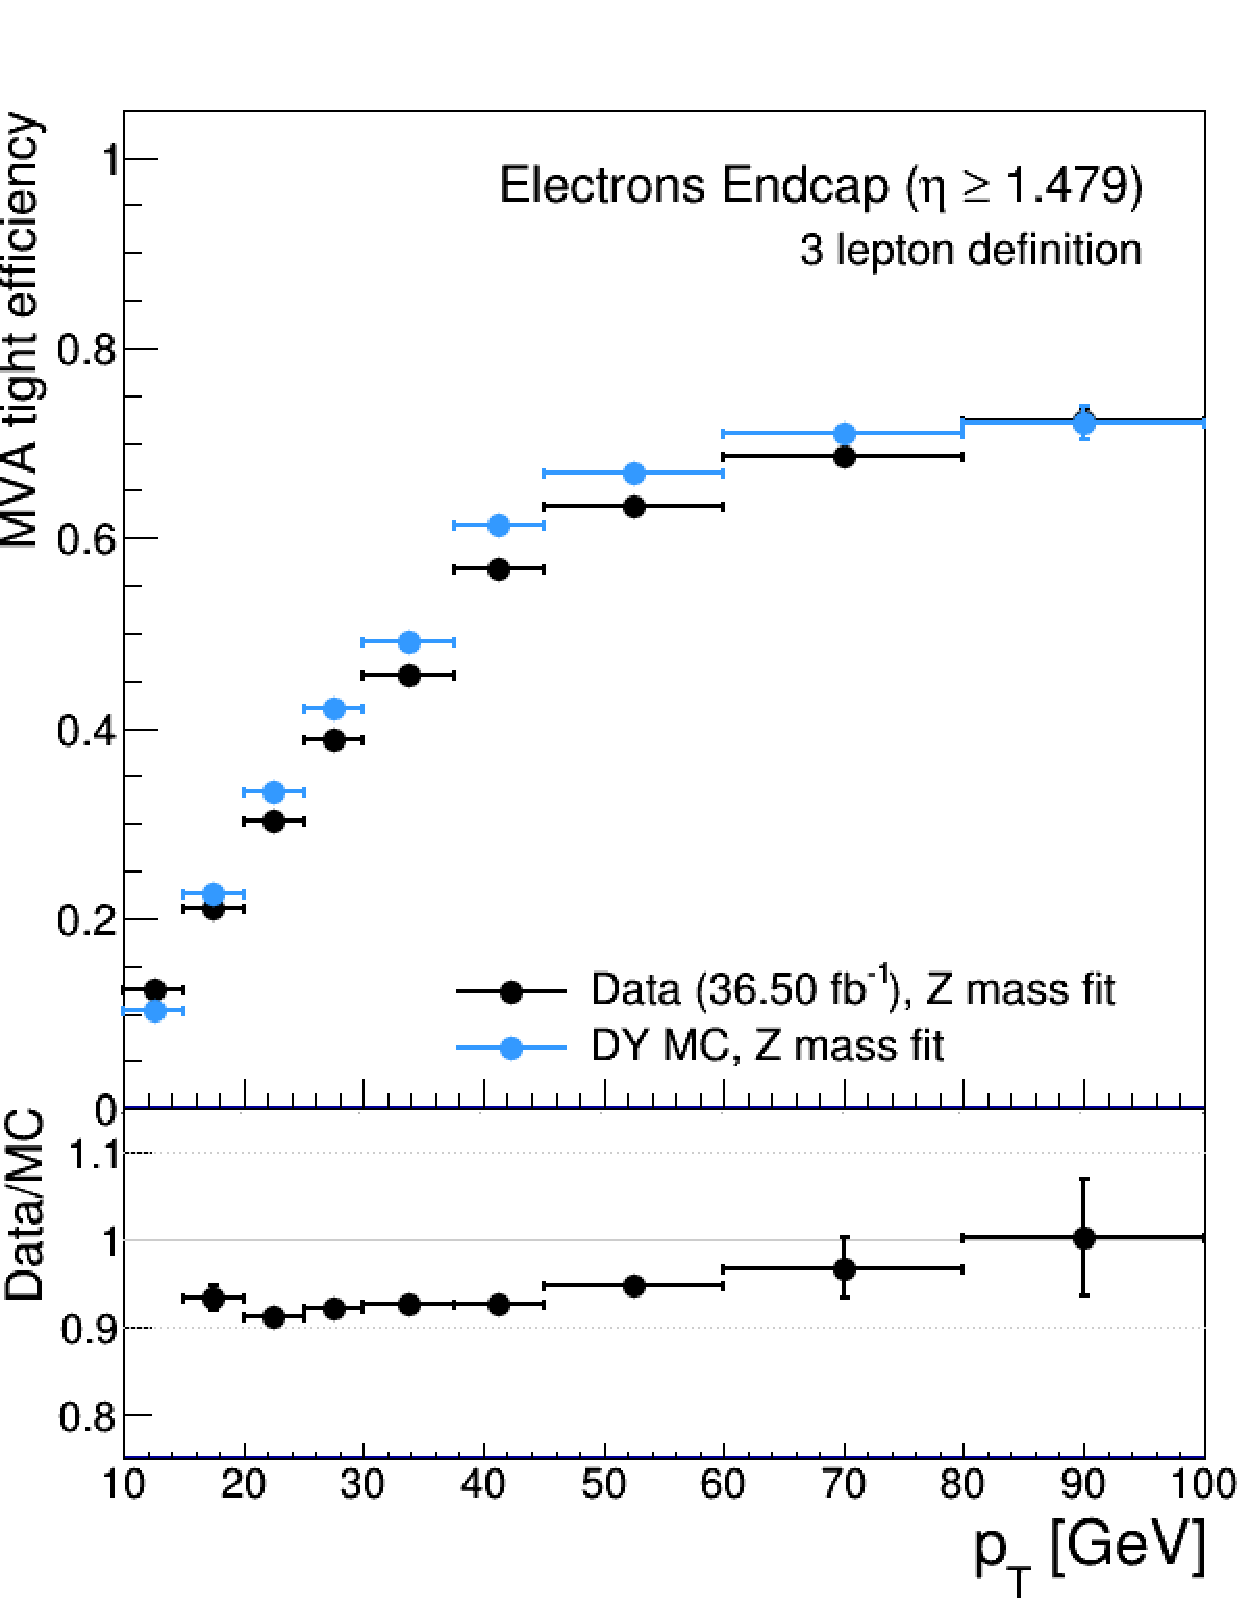
\includegraphics[width=0.31\linewidth]{plots_leptons/lepmva_efficiency/tnp_eff_ee_3l_pt.pdf}
\caption{Tight vs loose selection efficiencies for electrons, for the three lepton channel (\ie\ not including the tight-charge requirement).}
\label{fig:electronMVAEff_3l}
\end{figure}

\begin{figure}[!ht]
\centering
  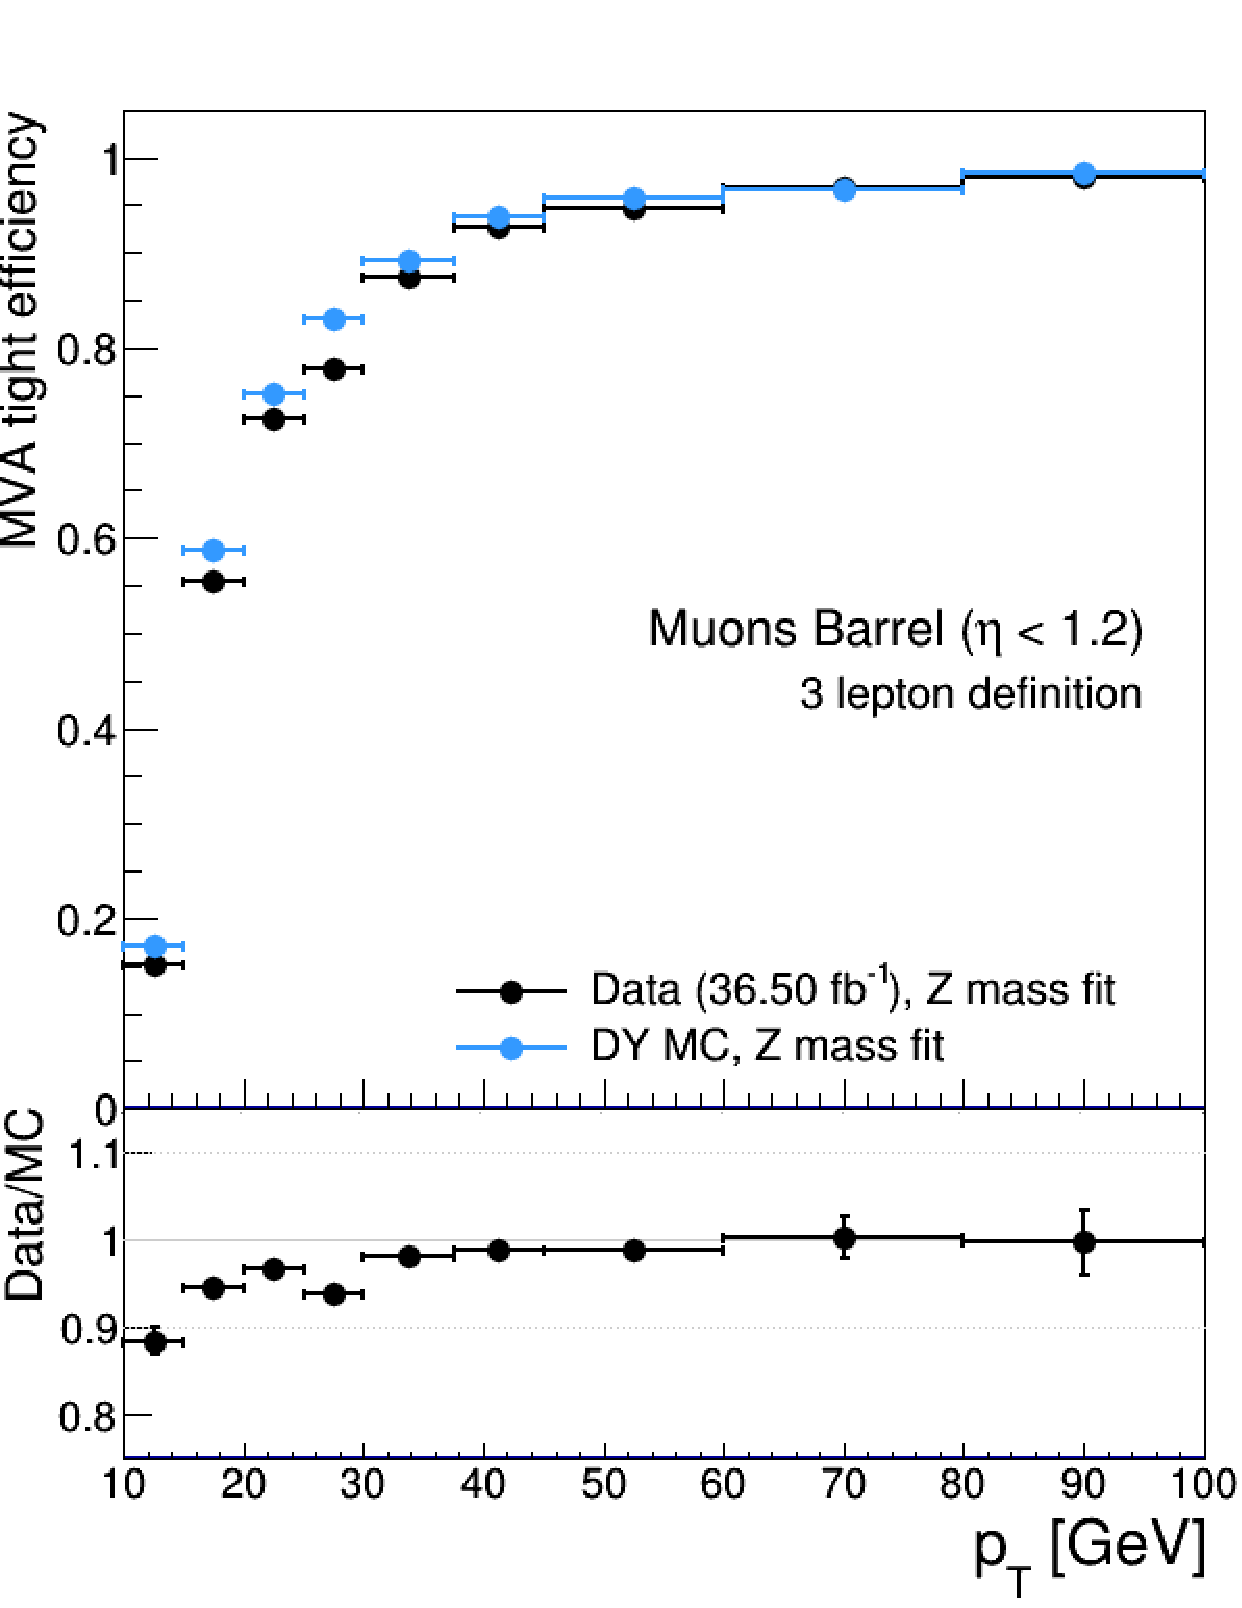
\includegraphics[width=0.31\linewidth]{plots_leptons/lepmva_efficiency/tnp_eff_mb_3l_pt.pdf}
  \includegraphics[width=0.31\linewidth]{plots_leptons/lepmva_efficiency/tnp_eff_me_3l_pt.pdf}
\caption{Tight vs loose selection efficiencies for muons, for the three lepton channel (\ie\ not including the tight-charge requirement).}
\label{fig:muonMVAEff_3l}
\end{figure}

We use these ($\eta$,$\pt$) dependent scale factors to correct the simulation. 
%A flat uncertainty of 3$\%$ which is of the order of the current statistical uncertainty is assigned to these scale factors. %% FIXME: Update the 3% number?
